\documentclass[lettersize,journal]{IEEEtran}
\def\MakeUppercaseUnsupportedInPdfStrings{\scshape}
\usepackage{amsmath,amsfonts}
\usepackage{algorithmic}
\usepackage{algorithm}
\usepackage{array}
\usepackage[caption=false,font=normalsize,labelfont=sf,textfont=sf]{subfig}
\usepackage{textcomp}
\usepackage{stfloats}
\usepackage{url}
\usepackage{hyperref}
\usepackage{verbatim}
\usepackage{graphicx}
\usepackage[backend=bibtex]{biblatex}
\usepackage[utf8]{inputenc}
\usepackage{pgfplots}
\usepackage{tikz}

\addbibresource{ref.bib}
\graphicspath{{./images/}}

\begin{document}
	
    \title{COMSOL Simulation of a Dual-axis MEMS Accelerometer with T-shape Beams}

    \author{Leonardo Bove\\
            \textit{Dipartimento di Ingegneria dell'Informazione}\\
            \textit{University of Pisa}\\
            \texttt{l.bove3@studenti.unipi.it}}

    \maketitle
	
    \begin{abstract}
        This paper presents the mechanical response of a MEMS dual-axis accelerometer with T-shaped beams for different values of X and Y axes accelerations. The original design idea and simulation are taken from an excerpt from the \textit{Proceedings of the 2015 COMSOL} Conference in Boston \cite{original}. The aim of this paper is to validate the results obtained in the reference through a COMSOL 6.0 Multiphysics simulation. The results show the inertial mass displacement and the induced stress. Beams equivalent elastic constants and displacement sensitivities to accelerations (\(S_{x}\), \(S_{y}\)) along X and Y axes were evaluated and compared to theoretical forecasts. Accelerations up to 50g were simulated. Moreover, the dependence of the  sensitivity along the X axis was evaluated for different values of the spring arms' dimensions \(w_{bx}\) and \(t_{bx}\). The obtained results are compared with the theoretical models proposed in the referenced paper.
    \end{abstract}
	
    \section{Introduction}
        \IEEEPARstart{N}{owadays}, MEMS accelerometers have an extensive applications range: consumer electronics, automotive systems, aerospace, and robotics. Small size, together with low power consumption and cost-effectiveness, turn them into the basis in inertial navigation and motion sensing. One critical evolution in the technology for MEMS accelerometers involves the development of dual-axis devices that can measure accelerations along two orthogonal axes in a single package. These designs improve integration efficiency and reduce the complexity of aligning several single-axis accelerometers.
        
        This report focuses on the analysis and optimization of a MEMS dual-axis accelerometer featuring T-shaped beams. The special geometry of these beams allows for the measurement of accelerations along both the X and Y axes through differential capacitance sensing. Theoretical basics of the accelerometer design, as mentioned in the referred article, are modeled and simulated in COMSOL Multiphysics.
        
        The main objectives of this study are:
        \begin{itemize}
        \item Calculating the displacement of the inertial mass and the induced stress for several acceleration inputs along both the X and Y axes. The range of accelerations is the same as the one simulated in the original paper, i.e. up to 50g in both directions.
        \item Obtaining the equivalent elastic constants of the beams and the device displacement sensitivity to accelerations, \(S_{x}\) and \(S_{y}\), in both axes.
        \item Carrying out a parametric analysis to study the dependence of sensitivity, \(S_{dx}\), on the spring arm dimensions \(w_{bx}\) and \(t_{bx}\).
        \item Comparing simulation results with theoretical predictions in order to validate the model and identify areas for possible design improvements.
        \end{itemize}
        
    \section{Structure Design and Analysis}
        The structure of the analysed device is shown in figure \ref{fig:dev-struct}. This accelerometer is designed to be fabricated with polysilcon surface-micromachining. The whole device is symmetric vertically and horizontally: these symmetries will be exploited later to reduce the COMSOL model size.
        
        The central movable mass is anchored through two T-shape beams. Each T-shape beam consists of one straight beam and two folded beams.
        
        Attached to the central mass, there are 64 movable fingers, divided into 8 groups. Each side of the central mass has 2 groups of fingers. Each of them faces one fixed finger and the capacitance between those is used to sense the external acceleration. The vertical fingers (aligned along the Y axis) together with the straight beams are used to sense acceleration along X direction, so they are called X-beams and X-capacitance groups. On the other hand, the horizontal fingers (aligned along the X axis) together with the folded beams are used to sense acceleration along Y direction, so they are called Y-beams and Y-capacitance groups. Due to the symmetry of the device, two of the four groups of X movable fingers have fixed fingers on the left side, whereas the other two groups have them on the right. Similarly, this apply to Y-movable fingers groups: two of them have fixed fingers in the upper side, the other two on the down side. This is helpful for obtaining a differential capacitance, as will be explained in section \ref{sssec:capacity}.
        
        
        \begin{figure}[h!]
            \centering
            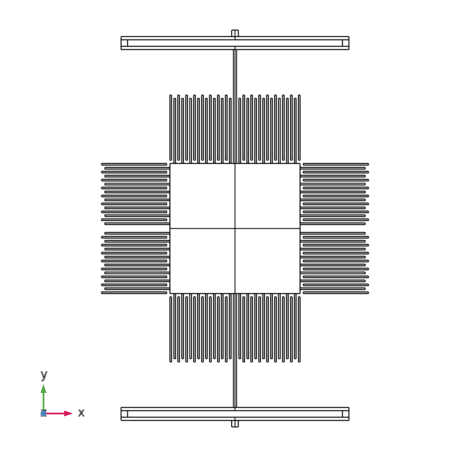
\includegraphics[width=1.0\linewidth]{full_device_geometry.png}
            \caption{Device structure.}
            \label{fig:dev-struct}
        \end{figure}
        
        \subsection{Device Geometrical Sizing}\label{ssec:geometry}
        A detailed view of the geometrical model used in this COMSOL simulation is presented in figure \ref{fig:dev_quotes}. As anticipated, in order to reduce the size of the model, only \(\frac{1}{8}\) of the whole device was simulated, taking advantage of the symmetries along X, Y and Z axes.
        
        \begin{figure}[h!]
            \centering
            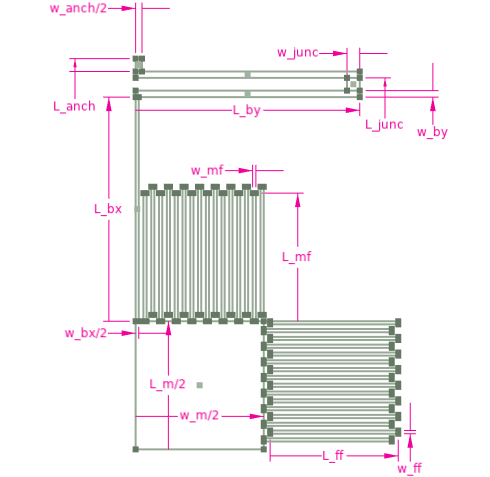
\includegraphics[width=1.0\linewidth]{device_size.png}
            \caption{Device dimensions.}
            \label{fig:dev_quotes}
        \end{figure}
        
        Table \ref{tab:size} shows all the geometrical parameters of the device, which are identical to those used in \cite{original}. The only dimensions that were missing are those of the folded beams junction element.
        
        \begin{table}[h!]
            \renewcommand{\arraystretch}{1.5}
            \centering
            \caption{Device components dimensions}
            \label{tab:size}
            \begin{tabular}{|c|c|c|c|}
                \hline
                \textbf{Components}   & \textbf{Quantity} & \textbf{Length (\(\mu m\))} & \textbf{Width (\(\mu m\))} \\ \hline
                Central mass          & 1                 & 800                  & 800                 \\ \hline
                Movable fingers       & 64                & 400                  & 10                  \\ \hline
                Fixed fingers         & 64                & 400                  & 10                  \\ \hline
                Folded beam segments  & 8                 & 700                  & 20                  \\ \hline
                Folded beam junctions & 4                 & 40                   & 40                  \\ \hline
                Straight beams        & 2                 & 700                  & 20                  \\ \hline
                Anchors               & 2                 & 40                   & 40                  \\ \hline
            \end{tabular}
        \end{table}
        
        The whole geometrical description of the device was parametrized on COMSOL, in order to make it more flexible and allow for geometrical parametric sweeps. The parameters labels used, as shown in figure \ref{fig:dev_quotes}, are the following:
        
        \begin{itemize}
            \item \(L_m, w_m, t_m\): length, width and thickness of the central mass.
            \item \(L_{bx}, w_{bx}, t_{bx}\): length, width and thickness of the straight X beam.
            \item \(L_{by}, w_{by}, t_{by}\): length, width and thickness of the folded Y beams segments.
            \item \(L_{junc}, w_{junc}\): length and width of the folded Y beams junctions. The thickness is the same as the other segments.
            \item \(L_{anch}, w_{anch}\): length and width of the anchor. The thickness is the same as the folded beams.
            \item \(L_{mf}, w_{mf}, t_{mf}\): length, width and thickness of the movable fingers.
            \item \(L_{ff}, w_{ff}\): length and width of the fixed fingers. The thickness is the same as the movable fingers.
        \end{itemize}
        
        The 8 fixed fingers at the vertices of the central mass are assumed to be aligned with the side of the mass itself, as shown in figure \ref{fig:ff-detail}.
        
        \begin{figure}
            \centering
            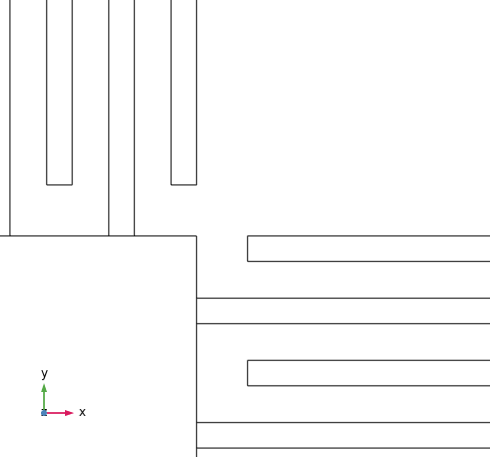
\includegraphics[width=1.0\linewidth]{device_ff_detail.png}
            \caption{Fixed fingers alignment detail.}
            \label{fig:ff-detail}
        \end{figure}
        
        The fingers of each group are assumed to be equally spaced and this spacing is the same for both the vertical and the horizontal groups. This spacing is parametrically defined from the available space for the movable fingers in the upper mass side, where the width of the straight beam must be taken into account. The free space between each fixed finger \(d\) is defined as follows:
        
        \begin{equation}
            d = \frac{\frac{L_m}{2}-8*(w_{mf}+w_{ff})-\frac{w_{bx}}{2}}{8}=
        \end{equation}
        
        Therefore, the pitch of the fixed (movable) fingers is equivalent to:
        
        \begin{equation}
            pitch = d+w_{mf}+w_{ff}
        \end{equation}
        The distance between each movable finger and its adjacent fixed fingers is not the same: as we can see from  figure \ref{fig:ff-detail}, in the upper-right side of the device the vertical movable fingers are positioned so that the fixed finger on the right is at distance \(\frac{d}{20}=1.4375\mu m\), whereas the one on the left is at distance \(d-\frac{d}{20}=27.3125\mu m\), which is much larger than the first one; on the other hand, thanks to the symmetry, the vertical movable fingers of the upper-left side are much closer the the fixed fingers on their left. Similarly, the same arrangement is used for the horizontal fingers, which are symmetric between the top and bottom sides. This will be helpful for the measurement of the differential capacitance, see section \ref{sssec:capacity}.
        
        Also the overlapping between the movable and fixed fingers had to be assumed and it was parametrically defined for both the vertical (\(L_{ov,v}\)) and horizontal (\(L_{ov,h}\)) fingers and set to \(L_{ov,v}=L_{ov,h}=380\mu m\).
        
        The outer air box that contains the device was defined to be larger than the maximum dimensions of the accelerometer by an offset of \(box_{offset}=50\mu m\). This is true for every side of the accelerometer, except for the three symmetry planes.
        
        \subsection{Theoretical Analysis}
        We now discuss the mathematical models used to predict the behaviour of this system.
        
        \subsubsection{Beams Stiffness}\label{sssec:stiffness}
        The simplified mechanical model of the system is presented in figure \ref{fig:model}.
        
        \begin{figure}[!h]
            \centering
            


\def \globalscale {0.800000}
\begin{tikzpicture}[y=1mm, x=1mm, yscale=\globalscale,xscale=\globalscale, every node/.append style={scale=\globalscale}, inner sep=0pt, outer sep=0pt]
  \path[draw=black,fill opacity=0.469072,line width=0.4mm] (31.418625, 
  251.886074) rectangle (51.418625, 231.886074);



  \path[draw=black,fill=black,opacity=1.0,fill opacity=0.469072,line 
  width=0.1mm] (26.418625, 276.986) rectangle (56.418625, 266.986);



  \path[draw=black,fill=black,fill opacity=0.469072,line width=0.099625mm,rotate
   around={-89.92615:(0.0, 297.0)}] (40.18483, 313.228563) rectangle (70.07226, 
  303.266085);



  \begin{scope}[line width=0.276301mm,cm={ 0.180962,-0.0,-0.0,0.180962,(6.416526, 200.550372)}]
    \path[draw=black,fill opacity=0.469072,line width=0.276301mm] (70.624773, 
  253.36302).. controls (76.294431, 258.393285) and (80.053537, 255.201658) .. 
  (82.641727, 252.020344).. controls (84.484435, 248.682459) and (86.803481, 
  245.753564) .. (85.662748, 236.176764).. controls (85.188319, 232.581153) and 
  (82.94443, 232.584503) .. (82.910261, 232.618672).. controls (82.910261, 
  232.618672) and (80.328288, 232.539002) .. (79.754972, 236.109631).. controls 
  (79.257444, 241.390824) and (79.417244, 246.672016) .. (82.641727, 
  251.953209).. controls (87.58241, 258.684842) and (93.076045, 255.092898) .. 
  (94.725812, 253.36302);



    \path[draw=black,fill opacity=0.469072,line width=0.276301mm] (83.826027, 
  253.295414).. controls (89.495685, 258.325679) and (93.254791, 255.134052) .. 
  (95.842981, 251.952738).. controls (97.685689, 248.614853) and (100.00474, 
  245.685958) .. (98.864002, 236.109158).. controls (98.389573, 232.513547) and 
  (96.145684, 232.516897) .. (96.111515, 232.551066).. controls (96.111515, 
  232.551066) and (93.529542, 232.471396) .. (92.956226, 236.042025).. controls 
  (92.458698, 241.323218) and (92.618498, 246.60441) .. (95.842981, 
  251.885603).. controls (100.78366, 258.617236) and (106.2773, 255.025292) .. 
  (107.92707, 253.295414);



    \path[draw=black,fill opacity=0.469072,line width=0.276301mm] (97.014234, 
  253.287703).. controls (102.68389, 258.317968) and (106.44299, 255.126341) .. 
  (109.03118, 251.945027).. controls (110.87389, 248.607142) and (113.19294, 
  245.678247) .. (112.0522, 236.101447).. controls (111.57777, 232.505836) and 
  (109.33388, 232.509186) .. (109.29972, 232.543355).. controls (109.29972, 
  232.543355) and (106.71774, 232.463685) .. (106.14443, 236.034314).. controls 
  (105.6469, 241.315507) and (105.8067, 246.596699) .. (109.03118, 251.877892)..
   controls (113.97186, 258.609525) and (119.4655, 255.017581) .. (121.11527, 
  253.287703);



  \end{scope}
  \path[draw=black,fill opacity=0.469072,line width=0.2mm] (19.267405, 
  246.448236).. controls (18.957553, 246.1935) and (18.629144, 245.837249) .. 
  (18.495366, 243.997852) -- (16.246383, 243.997852);



  \path[draw=black,fill opacity=0.469072,line width=0.2mm] (28.263337, 
  246.456629).. controls (28.787012, 245.910119) and (29.10366, 245.180955) .. 
  (29.001529, 243.919239) -- (31.418625, 243.919239);



  \begin{scope}[line width=0.276301mm,cm={ 0.0,-0.180962,0.180962,0.0,(0.087883, 276.721857)}]
    \path[draw=black,fill opacity=0.469072,line width=0.276301mm] (70.624773, 
  253.36302).. controls (76.294431, 258.393285) and (80.053537, 255.201658) .. 
  (82.641727, 252.020344).. controls (84.484435, 248.682459) and (86.803481, 
  245.753564) .. (85.662748, 236.176764).. controls (85.188319, 232.581153) and 
  (82.94443, 232.584503) .. (82.910261, 232.618672).. controls (82.910261, 
  232.618672) and (80.328288, 232.539002) .. (79.754972, 236.109631).. controls 
  (79.257444, 241.390824) and (79.417244, 246.672016) .. (82.641727, 
  251.953209).. controls (87.58241, 258.684842) and (93.076045, 255.092898) .. 
  (94.725812, 253.36302);



    \path[draw=black,fill opacity=0.469072,line width=0.276301mm] (83.826027, 
  253.295414).. controls (89.495685, 258.325679) and (93.254791, 255.134052) .. 
  (95.842981, 251.952738).. controls (97.685689, 248.614853) and (100.00474, 
  245.685958) .. (98.864002, 236.109158).. controls (98.389573, 232.513547) and 
  (96.145684, 232.516897) .. (96.111515, 232.551066).. controls (96.111515, 
  232.551066) and (93.529542, 232.471396) .. (92.956226, 236.042025).. controls 
  (92.458698, 241.323218) and (92.618498, 246.60441) .. (95.842981, 
  251.885603).. controls (100.78366, 258.617236) and (106.2773, 255.025292) .. 
  (107.92707, 253.295414);



    \path[draw=black,fill opacity=0.469072,line width=0.276301mm] (97.014234, 
  253.287703).. controls (102.68389, 258.317968) and (106.44299, 255.126341) .. 
  (109.03118, 251.945027).. controls (110.87389, 248.607142) and (113.19294, 
  245.678247) .. (112.0522, 236.101447).. controls (111.57777, 232.505836) and 
  (109.33388, 232.509186) .. (109.29972, 232.543355).. controls (109.29972, 
  232.543355) and (106.71774, 232.463685) .. (106.14443, 236.034314).. controls 
  (105.6469, 241.315507) and (105.8067, 246.596699) .. (109.03118, 251.877892)..
   controls (113.97186, 258.609525) and (119.4655, 255.017581) .. (121.11527, 
  253.287703);



  \end{scope}
  \path[draw=black,fill opacity=0.469072,line width=0.2mm] (45.985747, 
  263.870978).. controls (45.731011, 264.18083) and (45.37476, 264.509239) .. 
  (43.535363, 264.643017) -- (43.535363, 266.892);



  \path[draw=black,fill opacity=0.469072,line width=0.2mm] (45.99414, 
  254.875046).. controls (45.44763, 254.351371) and (44.718466, 254.034723) .. 
  (43.45675, 254.136854) -- (43.45675, 251.719758);



  \begin{scope}[line width=0.2mm]
    \path[draw=black,fill opacity=0.469072,line width=0.2mm] (25.135416, 
  240.114581) -- (19.843749, 240.114581) -- (19.843749, 234.822915) -- 
  (25.135416, 234.822915);



    \path[draw=black,fill opacity=0.469072,line width=0.2mm] (22.507045, 
  240.114581) -- (22.507045, 234.822915) -- (22.507045, 237.468748) -- 
  (31.368625, 237.468748);



    \path[draw=black,fill opacity=0.469072,line width=0.2mm] (19.843749, 
  237.468748) -- (16.305308, 237.468748);



  \end{scope}
  \begin{scope}[line width=0.2mm,cm={ 0.0,-1.0,1.0,0.0,(-200.496748, 283.285308)}]
    \path[draw=black,fill opacity=0.469072,line width=0.2mm] (25.135416, 
  240.114581) -- (19.843749, 240.114581) -- (19.843749, 234.822915) -- 
  (25.135416, 234.822915);



    \path[draw=black,fill opacity=0.469072,line width=0.2mm] (22.507045, 
  240.114581) -- (22.507045, 234.822915) -- (22.507045, 237.468748) -- 
  (31.368625, 237.468748);



    \path[draw=black,fill opacity=0.469072,line width=0.2mm] (19.843749, 
  237.468748) -- (16.305308, 237.468748);



  \end{scope}
  \begin{scope}[cm={ 0.781153,-0.0,-0.0,0.781153,(39.521882, 10.953651)}]
    \begin{scope}[fill=black,cm={ 0.352778,-0.0,-0.0,0.352778,(-80.7677, 204.166534)}]
      \begin{scope}[fill=black,shift={(228.479, -41.444)}]
        \path[fill=black] (3.546875, 302.046875).. controls (3.578125, 
  302.140625) and (4.015625, 303.015625) .. (4.65625, 303.5625).. controls 
  (5.09375, 303.96875) and (5.6875, 304.25) .. (6.359375, 304.25).. controls 
  (7.046875, 304.25) and (7.28125, 303.734375) .. (7.28125, 303.046875).. 
  controls (7.28125, 302.9375) and (7.28125, 302.59375) .. (7.078125, 301.78125)
   -- (6.640625, 300.015625).. controls (6.515625, 299.5) and (6.1875, 
  298.21875) .. (6.140625, 298.03125).. controls (6.078125, 297.78125) and 
  (5.96875, 297.328125) .. (5.96875, 297.265625).. controls (5.96875, 
  297.015625) and (6.171875, 296.828125) .. (6.421875, 296.828125).. controls 
  (6.9375, 296.828125) and (7.03125, 297.21875) .. (7.1875, 297.84375) -- 
  (8.21875, 301.953125).. controls (8.25, 302.09375) and (9.140625, 304.25) .. 
  (11.03125, 304.25).. controls (11.71875, 304.25) and (11.96875, 303.734375) ..
   (11.96875, 303.046875).. controls (11.96875, 302.078125) and (11.296875, 
  300.203125) .. (10.921875, 299.171875).. controls (10.765625, 298.75) and 
  (10.671875, 298.53125) .. (10.671875, 298.21875).. controls (10.671875, 
  297.453125) and (11.203125, 296.828125) .. (12.03125, 296.828125).. controls 
  (13.640625, 296.828125) and (14.234375, 299.359375) .. (14.234375, 
  299.46875).. controls (14.234375, 299.546875) and (14.171875, 299.625) .. 
  (14.0625, 299.625).. controls (13.90625, 299.625) and (13.890625, 299.5625) ..
   (13.8125, 299.265625).. controls (13.40625, 297.890625) and (12.78125, 
  297.171875) .. (12.09375, 297.171875).. controls (11.921875, 297.171875) and 
  (11.640625, 297.1875) .. (11.640625, 297.734375).. controls (11.640625, 
  298.1875) and (11.84375, 298.734375) .. (11.921875, 298.921875).. controls 
  (12.21875, 299.75) and (13.0, 301.78125) .. (13.0, 302.78125).. controls 
  (13.0, 303.8125) and (12.390625, 304.59375) .. (11.09375, 304.59375).. 
  controls (9.9375, 304.59375) and (9.0, 303.9375) .. (8.3125, 302.921875).. 
  controls (8.265625, 303.859375) and (7.703125, 304.59375) .. (6.40625, 
  304.59375).. controls (4.875, 304.59375) and (4.0625, 303.515625) .. (3.75, 
  303.078125).. controls (3.703125, 304.0625) and (3.0, 304.59375) .. (2.234375,
   304.59375).. controls (1.734375, 304.59375) and (1.34375, 304.359375) .. 
  (1.015625, 303.703125).. controls (0.703125, 303.078125) and (0.46875, 
  302.03125) .. (0.46875, 301.953125).. controls (0.46875, 301.890625) and 
  (0.53125, 301.796875) .. (0.65625, 301.796875).. controls (0.796875, 
  301.796875) and (0.8125, 301.828125) .. (0.90625, 302.21875).. controls 
  (1.171875, 303.234375) and (1.5, 304.25) .. (2.1875, 304.25).. controls 
  (2.578125, 304.25) and (2.71875, 303.96875) .. (2.71875, 303.453125).. 
  controls (2.71875, 303.078125) and (2.546875, 302.40625) .. (2.421875, 
  301.875) -- (1.953125, 300.015625).. controls (1.875, 299.6875) and (1.6875, 
  298.90625) .. (1.59375, 298.59375).. controls (1.484375, 298.15625) and 
  (1.296875, 297.34375) .. (1.296875, 297.265625).. controls (1.296875, 
  297.015625) and (1.484375, 296.828125) .. (1.734375, 296.828125).. controls 
  (1.953125, 296.828125) and (2.1875, 296.9375) .. (2.328125, 297.1875).. 
  controls (2.359375, 297.28125) and (2.515625, 297.875) .. (2.59375, 298.21875)
   -- (2.984375, 299.765625) -- cycle(3.546875, 302.046875);



      \end{scope}
    \end{scope}
  \end{scope}
  \begin{scope}[cm={ 0.645814,-0.0,-0.0,0.645814,(22.128244, 59.757554)}]
    \begin{scope}[fill=black,cm={ 0.352778,-0.0,-0.0,0.352778,(-80.7315, 202.628634)}]
      \begin{scope}[fill=black,shift={(227.892, -41.444)}]
        \path[fill=black] (4.84375, 308.515625).. controls (4.859375, 
  308.593755) and (4.890625, 308.6875) .. (4.890625, 308.78125).. controls 
  (4.890625, 308.953125) and (4.71875, 308.953125) .. (4.6875, 308.953125).. 
  controls (4.671875, 308.953125) and (4.046875, 308.890625) .. (3.734375, 
  308.859375).. controls (3.4375, 308.843745) and (3.1875, 308.812505) .. 
  (2.875, 308.796875).. controls (2.46875, 308.765625) and (2.34375, 308.750005)
   .. (2.34375, 308.4375).. controls (2.34375, 308.265625) and (2.515625, 
  308.265625) .. (2.6875, 308.265625).. controls (3.5625, 308.265625) and 
  (3.5625, 308.109375) .. (3.5625, 307.9375).. controls (3.5625, 307.85937) and 
  (3.5625, 307.828125) .. (3.484375, 307.515625) -- (1.015625, 297.671875).. 
  controls (0.953125, 297.40625) and (0.953125, 297.375) .. (0.953125, 
  297.28125).. controls (0.953125, 296.890625) and (1.234375, 296.828125) .. 
  (1.40625, 296.828125).. controls (1.890625, 296.828125) and (2.0, 297.203125) 
  .. (2.140625, 297.734375) -- (2.9375, 300.953125).. controls (4.1875, 
  300.828125) and (4.921875, 300.3125) .. (4.921875, 299.484375).. controls 
  (4.921875, 299.375) and (4.921875, 299.3125) .. (4.875, 299.046875).. controls
   (4.796875, 298.796875) and (4.796875, 298.578125) .. (4.796875, 298.5).. 
  controls (4.796875, 297.5) and (5.453125, 296.828125) .. (6.34375, 
  296.828125).. controls (7.125, 296.828125) and (7.546875, 297.546875) .. 
  (7.671875, 297.796875).. controls (8.046875, 298.421875) and (8.265625, 
  299.390625) .. (8.265625, 299.46875).. controls (8.265625, 299.546875) and 
  (8.203125, 299.625) .. (8.09375, 299.625).. controls (7.9375, 299.625) and 
  (7.921875, 299.546875) .. (7.859375, 299.265625).. controls (7.609375, 
  298.375) and (7.25, 297.171875) .. (6.375, 297.171875).. controls (6.03125, 
  297.171875) and (5.796875, 297.34375) .. (5.796875, 298.0).. controls 
  (5.796875, 298.328125) and (5.875, 298.703125) .. (5.9375, 298.96875).. 
  controls (6.015625, 299.265625) and (6.015625, 299.296875) .. (6.015625, 
  299.5).. controls (6.015625, 300.515625) and (5.09375, 301.078125) .. 
  (3.515625, 301.28125).. controls (4.125, 301.671875) and (4.75, 302.34375) .. 
  (5.0, 302.59375).. controls (5.96875, 303.703125) and (6.640625, 304.25) .. 
  (7.4375, 304.25).. controls (7.828125, 304.25) and (7.9375, 304.140625) .. 
  (8.0625, 304.046875).. controls (7.421875, 303.96875) and (7.1875, 303.53125) 
  .. (7.1875, 303.1875).. controls (7.1875, 302.765625) and (7.5, 302.625) .. 
  (7.75, 302.625).. controls (8.21875, 302.625) and (8.625, 303.03125) .. 
  (8.625, 303.578125).. controls (8.625, 304.078125) and (8.234375, 304.59375) 
  .. (7.453125, 304.59375).. controls (6.515625, 304.59375) and (5.734375, 
  303.921875) .. (4.515625, 302.546875).. controls (4.34375, 302.34375) and 
  (3.703125, 301.6875) .. (3.0625, 301.4375) -- cycle(4.84375, 308.515625);



      \end{scope}
    \end{scope}
    \begin{scope}[fill=black,cm={ 0.352778,-0.0,-0.0,0.352778,(-80.7315, 202.628634)}]
      \begin{scope}[fill=black,shift={(236.659, -44.026001)}]
        \path[fill=black] (5.671875, 301.875).. controls (5.28125, 301.8125) and
   (5.140625, 301.515625) .. (5.140625, 301.296875).. controls (5.140625, 301.0)
   and (5.359375, 300.90625) .. (5.53125, 300.90625).. controls (5.890625, 
  300.90625) and (6.140625, 301.21875) .. (6.140625, 301.546875).. controls 
  (6.140625, 302.046875) and (5.5625, 302.265625) .. (5.0625, 302.265625).. 
  controls (4.34375, 302.265625) and (3.9375, 301.546875) .. (3.828125, 
  301.328125).. controls (3.546875, 302.21875) and (2.8125, 302.265625) .. 
  (2.59375, 302.265625).. controls (1.375, 302.265625) and (0.734375, 
  300.703125) .. (0.734375, 300.4375).. controls (0.734375, 300.390625) and 
  (0.78125, 300.328125) .. (0.859375, 300.328125).. controls (0.953125, 
  300.328125) and (0.984375, 300.40625) .. (1.0, 300.453125).. controls 
  (1.40625, 301.78125) and (2.21875, 302.03125) .. (2.5625, 302.03125).. 
  controls (3.09375, 302.03125) and (3.203125, 301.53125) .. (3.203125, 
  301.25).. controls (3.203125, 300.984375) and (3.125, 300.703125) .. 
  (2.984375, 300.125) -- (2.578125, 298.5).. controls (2.40625, 297.78125) and 
  (2.0625, 297.125) .. (1.421875, 297.125).. controls (1.359375, 297.125) and 
  (1.0625, 297.125) .. (0.8125, 297.28125).. controls (1.25, 297.359375) and 
  (1.34375, 297.71875) .. (1.34375, 297.859375).. controls (1.34375, 298.09375) 
  and (1.15625, 298.25) .. (0.9375, 298.25).. controls (0.640625, 298.25) and 
  (0.328125, 297.984375) .. (0.328125, 297.609375).. controls (0.328125, 
  297.109375) and (0.890625, 296.875) .. (1.40625, 296.875).. controls 
  (1.984375, 296.875) and (2.390625, 297.328125) .. (2.640625, 297.828125).. 
  controls (2.828125, 297.125) and (3.4375, 296.875) .. (3.875, 296.875).. 
  controls (5.09375, 296.875) and (5.734375, 298.453125) .. (5.734375, 
  298.703125).. controls (5.734375, 298.765625) and (5.6875, 298.8125) .. 
  (5.625, 298.8125).. controls (5.515625, 298.8125) and (5.5, 298.75) .. 
  (5.46875, 298.65625).. controls (5.140625, 297.609375) and (4.453125, 297.125)
   .. (3.90625, 297.125).. controls (3.484375, 297.125) and (3.265625, 297.4375)
   .. (3.265625, 297.921875).. controls (3.265625, 298.1875) and (3.3125, 
  298.375) .. (3.5, 299.15625) -- (3.921875, 300.796875).. controls (4.09375, 
  301.5) and (4.5, 302.03125) .. (5.0625, 302.03125).. controls (5.078125, 
  302.03125) and (5.421875, 302.03125) .. (5.671875, 301.875) -- cycle(5.671875,
   301.875);



      \end{scope}
    \end{scope}
  \end{scope}
  \begin{scope}[cm={ 0.654181,-0.0,-0.0,0.654181,(20.553145, 39.18345)}]
    \begin{scope}[fill=black,cm={ 0.352778,-0.0,-0.0,0.352778,(-79.9751, 202.694834)}]
      \begin{scope}[fill=black,shift={(225.873, -41.444)}]
        \path[fill=black] (6.296875, 307.59375).. controls (6.453125, 
  308.234375) and (6.53125, 308.265625) .. (7.203125, 308.265625) -- (9.4375, 
  308.265625).. controls (11.375, 308.265625) and (11.375, 306.609375) .. 
  (11.375, 306.453125).. controls (11.375, 305.0625) and (9.984375, 303.28125) 
  .. (7.71875, 303.28125) -- (5.234375, 303.28125) -- cycle(9.21875, 
  303.140625).. controls (11.09375, 303.484375) and (12.796875, 304.796875) .. 
  (12.796875, 306.390625).. controls (12.796875, 307.734375) and (11.609375, 
  308.765625) .. (9.65625, 308.765625) -- (4.125, 308.765625).. controls 
  (3.8125, 308.765625) and (3.65625, 308.765625) .. (3.65625, 308.4375).. 
  controls (3.65625, 308.265625) and (3.8125, 308.265625) .. (4.0625, 
  308.265625).. controls (5.109375, 308.265625) and (5.109375, 308.125) .. 
  (5.109375, 307.9375).. controls (5.109375, 307.90625) and (5.109375, 
  307.796875) .. (5.046875, 307.53125) -- (2.71875, 298.28125).. controls 
  (2.5625, 297.671875) and (2.53125, 297.5) .. (1.328125, 297.5).. controls 
  (1.0, 297.5) and (0.828125, 297.5) .. (0.828125, 297.1875).. controls 
  (0.828125, 297.0) and (0.9375, 297.0) .. (1.28125, 297.0) -- (7.1875, 297.0)..
   controls (9.8125, 297.0) and (11.84375, 299.0) .. (11.84375, 300.734375).. 
  controls (11.84375, 302.140625) and (10.609375, 303.015625) .. (9.21875, 
  303.140625) -- cycle(6.765625, 297.5) -- (4.4375, 297.5).. controls (4.203125,
   297.5) and (4.171875, 297.5) .. (4.0625, 297.515625).. controls (3.875, 
  297.53125) and (3.859375, 297.5625) .. (3.859375, 297.703125).. controls 
  (3.859375, 297.828125) and (3.890625, 297.9375) .. (3.921875, 298.078125) -- 
  (5.125, 302.9375) -- (8.375, 302.9375).. controls (10.40625, 302.9375) and 
  (10.40625, 301.046875) .. (10.40625, 300.90625).. controls (10.40625, 299.25) 
  and (8.90625, 297.5) .. (6.765625, 297.5) -- cycle(6.765625, 297.5);



      \end{scope}
    \end{scope}
    \begin{scope}[fill=black,cm={ 0.352778,-0.0,-0.0,0.352778,(-79.9751, 202.694834)}]
      \begin{scope}[fill=black,shift={(238.679, -44.026001)}]
        \path[fill=black] (5.671875, 301.875).. controls (5.28125, 301.8125) and
   (5.140625, 301.515625) .. (5.140625, 301.296875).. controls (5.140625, 301.0)
   and (5.359375, 300.90625) .. (5.53125, 300.90625).. controls (5.890625, 
  300.90625) and (6.140625, 301.21875) .. (6.140625, 301.546875).. controls 
  (6.140625, 302.046875) and (5.5625, 302.265625) .. (5.0625, 302.265625).. 
  controls (4.34375, 302.265625) and (3.9375, 301.546875) .. (3.828125, 
  301.328125).. controls (3.546875, 302.21875) and (2.8125, 302.265625) .. 
  (2.59375, 302.265625).. controls (1.375, 302.265625) and (0.734375, 
  300.703125) .. (0.734375, 300.4375).. controls (0.734375, 300.390625) and 
  (0.78125, 300.328125) .. (0.859375, 300.328125).. controls (0.953125, 
  300.328125) and (0.984375, 300.40625) .. (1.0, 300.453125).. controls 
  (1.40625, 301.78125) and (2.21875, 302.03125) .. (2.5625, 302.03125).. 
  controls (3.09375, 302.03125) and (3.203125, 301.53125) .. (3.203125, 
  301.25).. controls (3.203125, 300.984375) and (3.125, 300.703125) .. 
  (2.984375, 300.125) -- (2.578125, 298.5).. controls (2.40625, 297.78125) and 
  (2.0625, 297.125) .. (1.421875, 297.125).. controls (1.359375, 297.125) and 
  (1.0625, 297.125) .. (0.8125, 297.28125).. controls (1.25, 297.359375) and 
  (1.34375, 297.71875) .. (1.34375, 297.859375).. controls (1.34375, 298.09375) 
  and (1.15625, 298.25) .. (0.9375, 298.25).. controls (0.640625, 298.25) and 
  (0.328125, 297.984375) .. (0.328125, 297.609375).. controls (0.328125, 
  297.109375) and (0.890625, 296.875) .. (1.40625, 296.875).. controls 
  (1.984375, 296.875) and (2.390625, 297.328125) .. (2.640625, 297.828125).. 
  controls (2.828125, 297.125) and (3.4375, 296.875) .. (3.875, 296.875).. 
  controls (5.09375, 296.875) and (5.734375, 298.453125) .. (5.734375, 
  298.703125).. controls (5.734375, 298.765625) and (5.6875, 298.8125) .. 
  (5.625, 298.8125).. controls (5.515625, 298.8125) and (5.5, 298.75) .. 
  (5.46875, 298.65625).. controls (5.140625, 297.609375) and (4.453125, 297.125)
   .. (3.90625, 297.125).. controls (3.484375, 297.125) and (3.265625, 297.4375)
   .. (3.265625, 297.921875).. controls (3.265625, 298.1875) and (3.3125, 
  298.375) .. (3.5, 299.15625) -- (3.921875, 300.796875).. controls (4.09375, 
  301.5) and (4.5, 302.03125) .. (5.0625, 302.03125).. controls (5.078125, 
  302.03125) and (5.421875, 302.03125) .. (5.671875, 301.875) -- cycle(5.671875,
   301.875);



      \end{scope}
    \end{scope}
  \end{scope}
  \begin{scope}[cm={ 0.564054,-0.0,-0.0,0.564054,(23.188108, 71.598636)}]
    \begin{scope}[shift={(9.79661, 41.806262)}]
      \begin{scope}[fill=black,cm={ 0.352778,-0.0,-0.0,0.352778,(-80.0658, 202.694834)}]
        \begin{scope}[fill=black,shift={(226.13, -41.444)}]
          \path[fill=black] (6.296875, 307.59375).. controls (6.453125, 
  308.234375) and (6.53125, 308.265625) .. (7.203125, 308.265625) -- (9.4375, 
  308.265625).. controls (11.375, 308.265625) and (11.375, 306.609375) .. 
  (11.375, 306.453125).. controls (11.375, 305.0625) and (9.984375, 303.28125) 
  .. (7.71875, 303.28125) -- (5.234375, 303.28125) -- cycle(9.21875, 
  303.140625).. controls (11.09375, 303.484375) and (12.796875, 304.796875) .. 
  (12.796875, 306.390625).. controls (12.796875, 307.734375) and (11.609375, 
  308.765625) .. (9.65625, 308.765625) -- (4.125, 308.765625).. controls 
  (3.8125, 308.765625) and (3.65625, 308.765625) .. (3.65625, 308.4375).. 
  controls (3.65625, 308.265625) and (3.8125, 308.265625) .. (4.0625, 
  308.265625).. controls (5.109375, 308.265625) and (5.109375, 308.125) .. 
  (5.109375, 307.9375).. controls (5.109375, 307.90625) and (5.109375, 
  307.796875) .. (5.046875, 307.53125) -- (2.71875, 298.28125).. controls 
  (2.5625, 297.671875) and (2.53125, 297.5) .. (1.328125, 297.5).. controls 
  (1.0, 297.5) and (0.828125, 297.5) .. (0.828125, 297.1875).. controls 
  (0.828125, 297.0) and (0.9375, 297.0) .. (1.28125, 297.0) -- (7.1875, 297.0)..
   controls (9.8125, 297.0) and (11.84375, 299.0) .. (11.84375, 300.734375).. 
  controls (11.84375, 302.140625) and (10.609375, 303.015625) .. (9.21875, 
  303.140625) -- cycle(6.765625, 297.5) -- (4.4375, 297.5).. controls (4.203125,
   297.5) and (4.171875, 297.5) .. (4.0625, 297.515625).. controls (3.875, 
  297.53125) and (3.859375, 297.5625) .. (3.859375, 297.703125).. controls 
  (3.859375, 297.828125) and (3.890625, 297.9375) .. (3.921875, 298.078125) -- 
  (5.125, 302.9375) -- (8.375, 302.9375).. controls (10.40625, 302.9375) and 
  (10.40625, 301.046875) .. (10.40625, 300.90625).. controls (10.40625, 299.25) 
  and (8.90625, 297.5) .. (6.765625, 297.5) -- cycle(6.765625, 297.5);



        \end{scope}
      \end{scope}
      \begin{scope}[fill=black,cm={ 0.352778,-0.0,-0.0,0.352778,(-80.0658, 202.694834)}]
        \begin{scope}[fill=black,shift={(238.936, -44.026001)}]
          \path[fill=black] (3.140625, 295.65625).. controls (2.828125, 
  295.203125) and (2.359375, 294.796875) .. (1.765625, 294.796875).. controls 
  (1.625, 294.796875) and (1.046875, 294.828125) .. (0.875, 295.375).. controls 
  (0.90625, 295.359375) and (0.96875, 295.359375) .. (0.984375, 295.359375).. 
  controls (1.34375, 295.359375) and (1.59375, 295.671875) .. (1.59375, 
  295.953125).. controls (1.59375, 296.21875) and (1.359375, 296.3125) .. 
  (1.1875, 296.3125).. controls (0.984375, 296.3125) and (0.578125, 296.171875) 
  .. (0.578125, 295.59375).. controls (0.578125, 294.984375) and (1.09375, 
  294.5625) .. (1.765625, 294.5625).. controls (2.96875, 294.5625) and 
  (4.171875, 295.65625) .. (4.5, 296.984375) -- (5.671875, 301.65625).. controls
   (5.6875, 301.703125) and (5.71875, 301.78125) .. (5.71875, 301.859375).. 
  controls (5.71875, 302.03125) and (5.5625, 302.15625) .. (5.390625, 
  302.15625).. controls (5.28125, 302.15625) and (5.03125, 302.109375) .. 
  (4.9375, 301.75) -- (4.046875, 298.234375).. controls (4.0, 298.015625) and 
  (4.0, 297.984375) .. (3.890625, 297.859375).. controls (3.65625, 297.53125) 
  and (3.265625, 297.125) .. (2.6875, 297.125).. controls (2.015625, 297.125) 
  and (1.953125, 297.78125) .. (1.953125, 298.09375).. controls (1.953125, 
  298.78125) and (2.28125, 299.703125) .. (2.609375, 300.5625).. controls 
  (2.734375, 300.90625) and (2.8125, 301.078125) .. (2.8125, 301.3125).. 
  controls (2.8125, 301.8125) and (2.453125, 302.265625) .. (1.859375, 
  302.265625).. controls (0.765625, 302.265625) and (0.328125, 300.53125) .. 
  (0.328125, 300.4375).. controls (0.328125, 300.390625) and (0.375, 300.328125)
   .. (0.453125, 300.328125).. controls (0.5625, 300.328125) and (0.578125, 
  300.375) .. (0.625, 300.546875).. controls (0.90625, 301.546875) and 
  (1.359375, 302.03125) .. (1.828125, 302.03125).. controls (1.9375, 302.03125) 
  and (2.140625, 302.03125) .. (2.140625, 301.640625).. controls (2.140625, 
  301.328125) and (2.015625, 300.984375) .. (1.828125, 300.53125).. controls 
  (1.25, 298.953125) and (1.25, 298.5625) .. (1.25, 298.28125).. controls (1.25,
   297.140625) and (2.0625, 296.875) .. (2.65625, 296.875).. controls (3.0, 
  296.875) and (3.4375, 296.984375) .. (3.84375, 297.4375) -- (3.859375, 
  297.421875).. controls (3.6875, 296.71875) and (3.5625, 296.25) .. (3.140625, 
  295.65625) -- cycle(3.140625, 295.65625);



        \end{scope}
      \end{scope}
    \end{scope}
  \end{scope}
  \begin{scope}[cm={ 0.557822,-0.0,-0.0,0.557822,(48.151519, 95.536661)}]
    \begin{scope}[fill=black,cm={ 0.352778,-0.0,-0.0,0.352778,(-80.8225, 202.628634)}]
      \begin{scope}[fill=black,shift={(228.14999, -41.444)}]
        \path[fill=black] (4.84375, 308.515625).. controls (4.859375, 
  308.593755) and (4.890625, 308.6875) .. (4.890625, 308.78125).. controls 
  (4.890625, 308.953125) and (4.71875, 308.953125) .. (4.6875, 308.953125).. 
  controls (4.671875, 308.953125) and (4.046875, 308.890625) .. (3.734375, 
  308.859375).. controls (3.4375, 308.843745) and (3.1875, 308.812505) .. 
  (2.875, 308.796875).. controls (2.46875, 308.765625) and (2.34375, 308.750005)
   .. (2.34375, 308.4375).. controls (2.34375, 308.265625) and (2.515625, 
  308.265625) .. (2.6875, 308.265625).. controls (3.5625, 308.265625) and 
  (3.5625, 308.109375) .. (3.5625, 307.9375).. controls (3.5625, 307.85937) and 
  (3.5625, 307.828125) .. (3.484375, 307.515625) -- (1.015625, 297.671875).. 
  controls (0.953125, 297.40625) and (0.953125, 297.375) .. (0.953125, 
  297.28125).. controls (0.953125, 296.890625) and (1.234375, 296.828125) .. 
  (1.40625, 296.828125).. controls (1.890625, 296.828125) and (2.0, 297.203125) 
  .. (2.140625, 297.734375) -- (2.9375, 300.953125).. controls (4.1875, 
  300.828125) and (4.921875, 300.3125) .. (4.921875, 299.484375).. controls 
  (4.921875, 299.375) and (4.921875, 299.3125) .. (4.875, 299.046875).. controls
   (4.796875, 298.796875) and (4.796875, 298.578125) .. (4.796875, 298.5).. 
  controls (4.796875, 297.5) and (5.453125, 296.828125) .. (6.34375, 
  296.828125).. controls (7.125, 296.828125) and (7.546875, 297.546875) .. 
  (7.671875, 297.796875).. controls (8.046875, 298.421875) and (8.265625, 
  299.390625) .. (8.265625, 299.46875).. controls (8.265625, 299.546875) and 
  (8.203125, 299.625) .. (8.09375, 299.625).. controls (7.9375, 299.625) and 
  (7.921875, 299.546875) .. (7.859375, 299.265625).. controls (7.609375, 
  298.375) and (7.25, 297.171875) .. (6.375, 297.171875).. controls (6.03125, 
  297.171875) and (5.796875, 297.34375) .. (5.796875, 298.0).. controls 
  (5.796875, 298.328125) and (5.875, 298.703125) .. (5.9375, 298.96875).. 
  controls (6.015625, 299.265625) and (6.015625, 299.296875) .. (6.015625, 
  299.5).. controls (6.015625, 300.515625) and (5.09375, 301.078125) .. 
  (3.515625, 301.28125).. controls (4.125, 301.671875) and (4.75, 302.34375) .. 
  (5.0, 302.59375).. controls (5.96875, 303.703125) and (6.640625, 304.25) .. 
  (7.4375, 304.25).. controls (7.828125, 304.25) and (7.9375, 304.140625) .. 
  (8.0625, 304.046875).. controls (7.421875, 303.96875) and (7.1875, 303.53125) 
  .. (7.1875, 303.1875).. controls (7.1875, 302.765625) and (7.5, 302.625) .. 
  (7.75, 302.625).. controls (8.21875, 302.625) and (8.625, 303.03125) .. 
  (8.625, 303.578125).. controls (8.625, 304.078125) and (8.234375, 304.59375) 
  .. (7.453125, 304.59375).. controls (6.515625, 304.59375) and (5.734375, 
  303.921875) .. (4.515625, 302.546875).. controls (4.34375, 302.34375) and 
  (3.703125, 301.6875) .. (3.0625, 301.4375) -- cycle(4.84375, 308.515625);



      \end{scope}
    \end{scope}
    \begin{scope}[fill=black,cm={ 0.352778,-0.0,-0.0,0.352778,(-80.8225, 202.628634)}]
      \begin{scope}[fill=black,shift={(236.91701, -44.026001)}]
        \path[fill=black] (3.140625, 295.65625).. controls (2.828125, 
  295.203125) and (2.359375, 294.796875) .. (1.765625, 294.796875).. controls 
  (1.625, 294.796875) and (1.046875, 294.828125) .. (0.875, 295.375).. controls 
  (0.90625, 295.359375) and (0.96875, 295.359375) .. (0.984375, 295.359375).. 
  controls (1.34375, 295.359375) and (1.59375, 295.671875) .. (1.59375, 
  295.953125).. controls (1.59375, 296.21875) and (1.359375, 296.3125) .. 
  (1.1875, 296.3125).. controls (0.984375, 296.3125) and (0.578125, 296.171875) 
  .. (0.578125, 295.59375).. controls (0.578125, 294.984375) and (1.09375, 
  294.5625) .. (1.765625, 294.5625).. controls (2.96875, 294.5625) and 
  (4.171875, 295.65625) .. (4.5, 296.984375) -- (5.671875, 301.65625).. controls
   (5.6875, 301.703125) and (5.71875, 301.78125) .. (5.71875, 301.859375).. 
  controls (5.71875, 302.03125) and (5.5625, 302.15625) .. (5.390625, 
  302.15625).. controls (5.28125, 302.15625) and (5.03125, 302.109375) .. 
  (4.9375, 301.75) -- (4.046875, 298.234375).. controls (4.0, 298.015625) and 
  (4.0, 297.984375) .. (3.890625, 297.859375).. controls (3.65625, 297.53125) 
  and (3.265625, 297.125) .. (2.6875, 297.125).. controls (2.015625, 297.125) 
  and (1.953125, 297.78125) .. (1.953125, 298.09375).. controls (1.953125, 
  298.78125) and (2.28125, 299.703125) .. (2.609375, 300.5625).. controls 
  (2.734375, 300.90625) and (2.8125, 301.078125) .. (2.8125, 301.3125).. 
  controls (2.8125, 301.8125) and (2.453125, 302.265625) .. (1.859375, 
  302.265625).. controls (0.765625, 302.265625) and (0.328125, 300.53125) .. 
  (0.328125, 300.4375).. controls (0.328125, 300.390625) and (0.375, 300.328125)
   .. (0.453125, 300.328125).. controls (0.5625, 300.328125) and (0.578125, 
  300.375) .. (0.625, 300.546875).. controls (0.90625, 301.546875) and 
  (1.359375, 302.03125) .. (1.828125, 302.03125).. controls (1.9375, 302.03125) 
  and (2.140625, 302.03125) .. (2.140625, 301.640625).. controls (2.140625, 
  301.328125) and (2.015625, 300.984375) .. (1.828125, 300.53125).. controls 
  (1.25, 298.953125) and (1.25, 298.5625) .. (1.25, 298.28125).. controls (1.25,
   297.140625) and (2.0625, 296.875) .. (2.65625, 296.875).. controls (3.0, 
  296.875) and (3.4375, 296.984375) .. (3.84375, 297.4375) -- (3.859375, 
  297.421875).. controls (3.6875, 296.71875) and (3.5625, 296.25) .. (3.140625, 
  295.65625) -- cycle(3.140625, 295.65625);



      \end{scope}
    \end{scope}
  \end{scope}

\end{tikzpicture}

            \caption{Simplified mechanical model of the dual axis accelerometer.}
            \label{fig:model}
        \end{figure}
        
        Here, \(k_x\) and \(k_y\) are the \textbf{equivalent stiffness constants} of the springs that allow, respectively, displacements along the X axis and the Y axis; \(B_x\) and \(B_y\) are the equivalent damping constants along the two axis, but they are not relevant in this study, given that we are evaluating the steady state of the system; \(m\) is the total inertial mass, i.e. the mass of the central block and of the movable fingers. \(m\) is given by the following equation:
        
        \begin{equation}\label{eq:mass}
            m=\rho_{poly} \cdot (w_m l_m t_m + 64\cdot w_{mf} l_{mf} t_{mf})
        \end{equation}
        
        where we neglect the mass of the beams.
        If we now assume that all the displacement along the X axis is due to the bending of the two straight beams and that the displacement along the Y axis is due to deformation of the two folded beams, we can say that \(k_x\) is equal to the equivalent spring constant of the straight beams combined and \(k_y\) is the one of the folded beams. We will also assume that there is no cross stiffness constant, i.e. we can neglect any displacement along the X axis due to forces along the Y axis and vice versa.
        
        Given these hypothesis, we can model the straight beam to be rigidly attached to the end of the folded beam (which we supposed to be fixed for X accelerations) and to have a roller, i.e. a guided end, on the other side, due to the infinitely rigid central mass, as shown in figure \ref{fig:straight_beam_model}. We suppose that all the force due to the acceleration of the inertial mass is concentrated at the right end of the beam.
        
        \begin{figure}[!h]
            \centering
            


\def \globalscale {0.500000}
\begin{tikzpicture}[y=1mm, x=1mm, yscale=\globalscale,xscale=\globalscale, every node/.append style={scale=\globalscale}, inner sep=0pt, outer sep=0pt]
  \path[draw=black,fill=black,fill opacity=0.597938,line width=0.1mm] 
  (21.166666, 286.416667) rectangle (42.333332, 225.562503);



  \path[draw=black,fill=black,fill opacity=0.597938,line width=0.1mm] 
  (116.41666, 286.416664) rectangle (137.583326, 225.5625);



  \path[draw=black,fill opacity=0.64433,line width=0.3mm] (42.333333, 
  270.541667).. controls (79.374998, 270.541666) and (79.374998, 257.312499) .. 
  (111.125, 257.312499);



  \path[draw=black,fill opacity=0.64433,line width=0.3mm] (42.333329, 265.4).. 
  controls (79.374994, 265.399999) and (79.374994, 252.170832) .. (111.125, 
  252.170832);



  \path[draw=black,fill opacity=0.64433,line width=0.3mm] (111.125, 257.3125) --
   (111.125, 252.020831);



  \path[draw=black,fill opacity=0.64433,line width=0.3mm] (105.83333, 265.25) --
   (111.125, 265.25) -- (111.125, 244.083331) -- (105.83333, 244.083331);



  \path[draw=black,fill opacity=0.64433,line width=0.3mm] (113.77083, 
  259.958332) circle (2.645833mm);



  \path[draw=black,fill opacity=0.64433,line width=0.3mm] (113.77083, 
  249.524998) circle (2.645833mm);



  \path[draw=black,fill opacity=0.64433,line width=0.3mm] (66.247554, 231.03669)
   -- (50.372554, 231.03669);



  \path[draw=black,fill opacity=0.64433,line width=0.3mm] (66.247335, 230.67186)
   -- (66.247335, 246.54686);



  \begin{scope}[shift={(48.148565, -68.753059)}]
    \begin{scope}[fill=black,cm={ 0.352778,-0.0,-0.0,0.352778,(-81.8094, 204.166534)}]
      \begin{scope}[fill=black,shift={(231.43201, -41.444)}]
        \path[fill=black] (4.53125, 295.078125).. controls (4.0625, 294.421875) 
  and (3.390625, 293.828125) .. (2.546875, 293.828125).. controls (2.34375, 
  293.828125) and (1.515625, 293.859375) .. (1.25, 294.65625).. controls 
  (1.3125, 294.640625) and (1.390625, 294.640625) .. (1.421875, 294.640625).. 
  controls (1.953125, 294.640625) and (2.296875, 295.09375) .. (2.296875, 
  295.484375).. controls (2.296875, 295.875) and (1.96875, 296.015625) .. 
  (1.703125, 296.015625).. controls (1.421875, 296.015625) and (0.828125, 
  295.8125) .. (0.828125, 294.96875).. controls (0.828125, 294.09375) and 
  (1.5625, 293.484375) .. (2.546875, 293.484375).. controls (4.265625, 
  293.484375) and (6.015625, 295.078125) .. (6.484375, 296.984375) -- (8.171875,
   303.703125).. controls (8.203125, 303.78125) and (8.234375, 303.890625) .. 
  (8.234375, 303.984375).. controls (8.234375, 304.25) and (8.03125, 304.421875)
   .. (7.765625, 304.421875).. controls (7.609375, 304.421875) and (7.25, 
  304.359375) .. (7.109375, 303.828125) -- (5.84375, 298.78125).. controls 
  (5.75, 298.46875) and (5.75, 298.421875) .. (5.609375, 298.234375).. controls 
  (5.265625, 297.75) and (4.703125, 297.171875) .. (3.875, 297.171875).. 
  controls (2.90625, 297.171875) and (2.828125, 298.125) .. (2.828125, 
  298.578125).. controls (2.828125, 299.5625) and (3.28125, 300.890625) .. 
  (3.75, 302.125).. controls (3.9375, 302.625) and (4.046875, 302.875) .. 
  (4.046875, 303.21875).. controls (4.046875, 303.9375) and (3.53125, 304.59375)
   .. (2.6875, 304.59375).. controls (1.109375, 304.59375) and (0.46875, 
  302.09375) .. (0.46875, 301.953125).. controls (0.46875, 301.890625) and 
  (0.53125, 301.796875) .. (0.65625, 301.796875).. controls (0.8125, 301.796875)
   and (0.828125, 301.875) .. (0.890625, 302.109375).. controls (1.3125, 
  303.5625) and (1.96875, 304.25) .. (2.640625, 304.25).. controls (2.796875, 
  304.25) and (3.078125, 304.25) .. (3.078125, 303.6875).. controls (3.078125, 
  303.234375) and (2.890625, 302.734375) .. (2.640625, 302.078125).. controls 
  (1.796875, 299.828125) and (1.796875, 299.25) .. (1.796875, 298.84375).. 
  controls (1.796875, 297.203125) and (2.96875, 296.828125) .. (3.828125, 
  296.828125).. controls (4.328125, 296.828125) and (4.9375, 296.984375) .. 
  (5.546875, 297.625) -- (5.5625, 297.609375).. controls (5.296875, 296.59375) 
  and (5.125, 295.921875) .. (4.53125, 295.078125) -- cycle(4.53125, 295.078125);



      \end{scope}
    \end{scope}
  \end{scope}
  \begin{scope}[shift={(69.962982, -47.53127)}]
    \begin{scope}[fill=black,cm={ 0.352778,-0.0,-0.0,0.352778,(-81.6841, 204.166534)}]
      \begin{scope}[fill=black,shift={(231.061, -41.444)}]
        \path[fill=black] (8.15625, 304.03125).. controls (7.609375, 303.921875)
   and (7.40625, 303.515625) .. (7.40625, 303.1875).. controls (7.40625, 
  302.765625) and (7.734375, 302.625) .. (7.96875, 302.625).. controls 
  (8.484375, 302.625) and (8.84375, 303.078125) .. (8.84375, 303.546875).. 
  controls (8.84375, 304.265625) and (8.03125, 304.59375) .. (7.296875, 
  304.59375).. controls (6.25, 304.59375) and (5.671875, 303.5625) .. (5.515625,
   303.234375).. controls (5.109375, 304.53125) and (4.046875, 304.59375) .. 
  (3.734375, 304.59375).. controls (1.984375, 304.59375) and (1.046875, 
  302.34375) .. (1.046875, 301.953125).. controls (1.046875, 301.890625) and 
  (1.125, 301.796875) .. (1.234375, 301.796875).. controls (1.375, 301.796875) 
  and (1.40625, 301.90625) .. (1.453125, 301.96875).. controls (2.03125, 
  303.890625) and (3.1875, 304.25) .. (3.6875, 304.25).. controls (4.453125, 
  304.25) and (4.609375, 303.53125) .. (4.609375, 303.109375).. controls 
  (4.609375, 302.734375) and (4.515625, 302.34375) .. (4.3125, 301.515625) -- 
  (3.71875, 299.15625).. controls (3.46875, 298.125) and (2.96875, 297.171875) 
  .. (2.046875, 297.171875).. controls (1.96875, 297.171875) and (1.53125, 
  297.171875) .. (1.171875, 297.390625).. controls (1.796875, 297.515625) and 
  (1.921875, 298.03125) .. (1.921875, 298.234375).. controls (1.921875, 
  298.578125) and (1.671875, 298.796875) .. (1.34375, 298.796875).. controls 
  (0.9375, 298.796875) and (0.484375, 298.421875) .. (0.484375, 297.875).. 
  controls (0.484375, 297.15625) and (1.296875, 296.828125) .. (2.03125, 
  296.828125).. controls (2.859375, 296.828125) and (3.4375, 297.484375) .. 
  (3.8125, 298.1875).. controls (4.078125, 297.171875) and (4.9375, 296.828125) 
  .. (5.578125, 296.828125).. controls (7.328125, 296.828125) and (8.265625, 
  299.078125) .. (8.265625, 299.46875).. controls (8.265625, 299.546875) and 
  (8.203125, 299.625) .. (8.09375, 299.625).. controls (7.9375, 299.625) and 
  (7.921875, 299.53125) .. (7.875, 299.390625).. controls (7.40625, 297.875) and
   (6.40625, 297.171875) .. (5.625, 297.171875).. controls (5.03125, 297.171875)
   and (4.703125, 297.625) .. (4.703125, 298.328125).. controls (4.703125, 
  298.703125) and (4.765625, 298.984375) .. (5.046875, 300.109375) -- (5.640625,
   302.453125).. controls (5.90625, 303.484375) and (6.484375, 304.25) .. 
  (7.28125, 304.25).. controls (7.3125, 304.25) and (7.796875, 304.25) .. 
  (8.15625, 304.03125) -- cycle(8.15625, 304.03125);



      \end{scope}
    \end{scope}
  \end{scope}
  \path[draw=black,fill=black,line width=0.3mm] (66.247335, 246.546861) -- 
  (64.822913, 245.406248) -- (67.468747, 245.406248) -- cycle;



  \path[draw=black,fill=black,line width=0.3mm] (50.372554, 231.03669) -- 
  (50.27083, 229.531248) -- (48.947913, 230.854165) -- (50.27083, 232.177082) --
   cycle;




\end{tikzpicture}

            \caption{Straight beam model. On the right there is the central mass.}
            \label{fig:straight_beam_model}
        \end{figure}
        
        The equivalent stiffness constant of this type of structure, due to a force along the X axis concentrated at the right end, is well known in the scientific literature and is given by the following equation:
        
        \begin{equation}\label{eq:straight_beam_k_symbol}
            k_{straight} = 12\frac{EJ}{L^3}
        \end{equation}
        
        where \(E\) is the Young's modulus of the polysilicon, \(L\) is the length of the beam and \(J\) is the moment of inertia of the beam's section, due to a bending moment along the z axis (see the reference plane used in figure \ref{fig:straight_beam_model}). In our case:
        
        \begin{equation}\label{eq:j_straight}
            J=\frac{bh^3}{12}=\frac{t_{bx}w^3_{bx}}{12}
        \end{equation}
        
        Hence, the equivalent stiffness of one straight beam is
        
        \begin{equation}\label{eq:straight_beam_k_x}
            k_{straight,x} = \frac{Et_{bx}w^3_{bx}}{L^3_{bx}}
        \end{equation}
        
        Given that the two straight beams undergo the same displacement, thanks to the symmetry of the model, we can easily consider the two springs in parallel and the total x stiffness will be given by the sum of the two spring constants:
        
        \begin{equation}\label{eq:k_x}
            k_x = 2\cdot k_{straight,x}=2\frac{Et_{bx}w^3_{bx}}{L^3_{bx}}=31.5335N/m
        \end{equation}
        
        For what concerns the stiffness along the Y axis, we can model the two segments of the folded beam as in figure \ref{fig:straight_beam_model}, therefore each segment has the same stiffness as the straight beam, taking into account the different geometrical dimensions.
        
        \begin{equation}\label{eq:straight_beam_k_y}
            k_{straight,y} = \frac{Et_{by}w^3_{by}}{L^3_{by}}
        \end{equation}
        
        The two segments are attached one to the other through the junction segment, which is supposed to be infinitely rigid and not to be able to bend, due to its aspect ratio. For this reason we can model it as a roller. Given that the two segment are mechanically in series and they have the same spring constant, the total stiffness is half of a single one:
        
        \begin{equation}\label{eq:folded_k}
            k_{folded}=\frac{k_{straight,y}\cdot k_{straight,y}}{k_{straight,y}+k_{straight,y}}=\frac{k_{straight,y}}{2}
        \end{equation}
        
        Now, given that for each T beam there are two folded beams and that all of them undergo the same displacement (as absolute value), we can model these four springs as if they were in parallel and the total y stiffness is given by the following equation:
        
        \begin{equation}\label{eq:k_y}
            k_y = 4\cdot k_{folded}=4\frac{k_{straight,y}}{2}=2\frac{Et_{by}w^3_{by}}{L^3_{by}}=31.5335N/m
        \end{equation}
        
        However, we need to keep in mind that the COMSOL model will be only \(\frac{1}{8}\) of the total model, as explained in section \ref{ssec:geometry}. Therefore, the spring dimensions will be different and the inertial mass will be \(\frac{1}{8}\)
         of the total inertial mass. We can find an analytical relationships between the reduced spring constants and the complete ones, so that we can compare the output of the simulation with the theoretical model.
         
         Thanks to the symmetry of the model, we can affirm that the stiffness of the reduced springs will be \(\frac{1}{8}\) of the total corresponding springs, because it is possible to see all the reduced springs as if they were in parallel to each other.
         
         \begin{equation}\label{eq:k_x_red}
             k_{x,reduced}=\frac{k_x}{8}
         \end{equation}
         
         \begin{equation}\label{eq:k_y_red}
             k_{y,reduced}=\frac{k_y}{8}
         \end{equation}
         
         %Any object will have half of its thickness, because every domain is symmetric along the Z axis. The other dimensions can be seen in figure \ref{fig:dev_quotes}.
         
         %\begin{equation}\label{eq:k_x_red}
         %    k_{x,reduced}=\frac{E\frac{t_{bx}}{2}\left(\frac{w_{bx}}{2}\right)^3}{L^3_{bx}}=\frac{k_x}{32}
         %\end{equation}
         
         %\begin{equation}\label{eq:k_y_red}
         %    k_{y,reduced}=\frac{1}{2}\frac{E\frac{t_{by}}{2}w^3_{by}}{L^3_{by}}=\frac{k_y}{8}
         %\end{equation}
         
        This coefficients will be multiplied by the spring constants found in simulation.
        
        \subsubsection{Displacement Sensitivity To Accelerations}
        The \textbf{displacement sensitivity} is defined as the displacement of the movable fingers when \(1g\) of acceleration is applied. Therefore, considering the equivalent mechanical model of the system, we can evaluate the sensitivity along the two axes. Since we neglected the cross stiffness, the displacement is given by the following equations:
        
        \begin{equation}\label{eq:x_disp}
            \Delta x = \frac{F_x}{k_x}
        \end{equation}
        
        \begin{equation}\label{eq:y_disp}
            \Delta y = \frac{F_y}{k_y}
        \end{equation}
        
        where \(F_x\) and \(F_y\) are the equivalent forces along the respective axis, due to an acceleration of the inertial mass.
        Hence, the sensitivities:
        
        \begin{equation}\label{eq:x_sens}
            \begin{split}
                S_x & = \left. \Delta x\right|_{a_x=1g,a_y=0}=\left. \frac{ma_x}{k_x} \right|_{a_x=1g,a_y=0} \\
                & =\frac{\rho_{poly} \cdot (w_m l_m t_m + 64\cdot w_{mf} l_{mf} t_{mf})gL^3_{bx}}{2\cdot Et_{bx}w^3_{bx}} \\
                & = 0.002587\mu m
            \end{split}
        \end{equation}
        
        \begin{equation}\label{eq:y_sens}
            \begin{split}
                S_y & = \left. \Delta y\right|_{a_y=1g,a_x=0}=\left. \frac{ma_y}{k_y} \right|_{a_y=1g,a_x=0} \\
                & =\frac{\rho_{poly} \cdot (w_m l_m t_m + 64\cdot w_{mf} l_{mf} t_{mf})gL^3_{by}}{2\cdot Et_{by}w^3_{by}} \\
                & = 0.002587\mu m
            \end{split}
        \end{equation}
        
        \subsubsection{Capacitance Sensing}\label{sssec:capacity}
        As anticipated before, thanks to the mirrored position of the fixed fingers relative to the movable fingers (e.g. in the upper-right side fixed fingers are on the right of their respective movable fingers, whereas in the upper-left side the opposite happens) differential capacitance can be measured to sense the displacement of the mass due to inertial force.
        
        Each movable finger will have two equivalent parallel capacitances with the adjacent fixed fingers, if the fixed fingers are set at the same voltage. However, as shown in figure \ref{fig:ff-detail}, the capacitance with the nearest fixed finger is much greater than the other, which can therefore be neglected.
        
        When there is no acceleration, the capacitance gap between each movable finger and its nearest fixed finger is the same and equal to \(d_0=\frac{d}{20}\), therefore the differential capacitance between the left/right (top/bottom) X (Y) capacitance groups is zero.
        
        When a positive X axis acceleration is applied, due to inertial force, the movable fingers move towards right by a displacement x: the right capacitance gap is now \(d_r=d_0-x\), whereas the left capacitance gap is \(d_l=d_0+x\) (see figure \ref{fig:capacitance_drawing}).
        
        \begin{figure}[!h]
            \centering
            


\def \globalscale {1.000000}
\begin{tikzpicture}[y=1mm, x=1mm, yscale=\globalscale,xscale=\globalscale, every node/.append style={scale=\globalscale}, inner sep=0pt, outer sep=0pt]
  \path[draw=black,fill=black,fill opacity=0.35124,line width=0.1mm] (11.856247,
   226.935414) -- (11.856247, 236.19583) -- (17.147913, 236.19583) -- 
  (17.147913, 249.424997) -- (19.793747, 249.424997) -- (19.793747, 236.19583) 
  -- (31.699997, 236.19583) -- (31.699997, 249.424997) -- (34.34583, 249.424997)
   -- (34.34583, 236.19583) -- (40.960414, 236.19583) -- (40.960414, 226.935414)
   -- cycle;



  \path[draw=black,fill=black,fill opacity=0.35124,line width=0.1mm] (10.583333,
   255.989584).. controls (13.229166, 255.989584) and (13.229166, 255.989584) ..
   (13.229166, 255.989584) -- (13.229166, 238.791665) -- (10.583333, 238.791665)
   -- cycle;



  \path[draw=black,fill=black,fill opacity=0.35124,line width=0.1mm] (27.78125, 
  238.791665) -- (25.135416, 238.791665) -- (25.135416, 255.989584) -- 
  (27.78125, 255.989584) -- cycle;



  \path[draw=black,fill=black,fill opacity=0.35124,line width=0.1mm] (70.064581,
   226.935414) -- (70.064581, 236.19583) -- (64.772915, 236.19583) -- 
  (64.772915, 249.424997) -- (62.127081, 249.424997) -- (62.127081, 236.19583) 
  -- (50.220831, 236.19583) -- (50.220831, 249.424997) -- (47.574998, 
  249.424997) -- (47.574998, 236.19583) -- (40.960414, 236.19583) -- (40.960414,
   226.935414) -- cycle;



  \path[draw=black,fill=black,fill opacity=0.35124,line width=0.1mm] (68.791667,
   255.989584).. controls (66.145834, 255.989584) and (66.145834, 255.989584) ..
   (66.145834, 255.989584) -- (66.145834, 238.791665) -- (68.791667, 238.791665)
   -- cycle;



  \path[draw=black,fill=black,fill opacity=0.35124,line width=0.1mm] (51.59375, 
  238.791665) -- (54.239584, 238.791665) -- (54.239584, 255.989584) -- 
  (51.59375, 255.989584) -- cycle;



  \path[draw=black,fill=black,line width=0.1mm] (33.072916, 224.239582) -- 
  (48.947913, 224.239582) -- (48.947915, 224.768748) -- (49.741665, 224.239581) 
  -- (48.947915, 223.710414) -- (48.947913, 224.239582);



  \path[draw=black,fill=black,line width=0.1mm] (5.291666, 224.239582) -- 
  (9.260416, 224.239582) -- (9.260416, 224.504165) -- (9.789583, 224.239582) -- 
  (9.260416, 223.974998) -- (9.260416, 224.239582);



  \path[draw=black,fill=black,line width=0.1mm] (5.291666, 224.239582) -- 
  (5.291666, 228.208332) -- (5.027083, 228.208332) -- (5.291666, 228.737498) -- 
  (5.55625, 228.208332) -- (5.291666, 228.208332);



  \path[draw=black,fill=black,line width=0.1mm] (13.229166, 255.989584) -- 
  (13.229166, 261.28125);



  \path[draw=black,fill=black,line width=0.1mm] (17.197916, 249.374998) -- 
  (17.197916, 261.28125);



  \path[draw=black,line width=0.1mm] (16.933333, 261.016667) -- (17.462499, 
  261.545834) -- (17.197916, 261.28125) -- (13.229166, 261.28125) -- (13.49375, 
  261.545832) -- (12.964583, 261.016666);



  \path[draw=black,line width=0.1mm] (66.14583, 255.989584) -- (66.14583, 
  261.28125) -- (64.822913, 261.28125) -- (64.822913, 249.374998) -- (64.822913,
   261.28125) -- (65.087497, 261.545834) -- (64.55833, 261.016667);



  \path[draw=black,line width=0.1mm] (66.410413, 261.545834) -- (65.881247, 
  261.016667);



  \begin{scope}[cm={ 0.76353,-0.0,-0.0,0.76353,(10.451006, -1.894926)}]
    \begin{scope}[fill=black,cm={ 0.352778,-0.0,-0.0,0.352778,(-41.9502, 197.873034)}]
      \begin{scope}[fill=black,shift={(118.664, -19.525999)}]
        \path[fill=black] (4.0, 300.171875).. controls (3.640625, 300.09375) and
   (3.625, 299.78125) .. (3.625, 299.75).. controls (3.625, 299.578125) and 
  (3.765625, 299.453125) .. (3.9375, 299.453125).. controls (4.109375, 
  299.453125) and (4.375, 299.59375) .. (4.375, 299.9375).. controls (4.375, 
  300.390625) and (3.875, 300.515625) .. (3.578125, 300.515625).. controls 
  (3.21875, 300.515625) and (2.90625, 300.25) .. (2.71875, 299.9375).. controls 
  (2.546875, 300.359375) and (2.140625, 300.515625) .. (1.8125, 300.515625).. 
  controls (0.9375, 300.515625) and (0.453125, 299.515625) .. (0.453125, 
  299.296875).. controls (0.453125, 299.21875) and (0.515625, 299.1875) .. 
  (0.578125, 299.1875).. controls (0.671875, 299.1875) and (0.6875, 299.234375) 
  .. (0.703125, 299.328125).. controls (0.890625, 299.90625) and (1.375, 
  300.296875) .. (1.78125, 300.296875).. controls (2.09375, 300.296875) and 
  (2.25, 300.0625) .. (2.25, 299.78125).. controls (2.25, 299.625) and (2.15625,
   299.25) .. (2.09375, 299.0).. controls (2.03125, 298.765625) and (1.859375, 
  298.0625) .. (1.8125, 297.90625).. controls (1.703125, 297.484375) and 
  (1.421875, 297.140625) .. (1.0625, 297.140625).. controls (1.03125, 
  297.140625) and (0.828125, 297.140625) .. (0.65625, 297.25).. controls 
  (1.015625, 297.34375) and (1.015625, 297.671875) .. (1.015625, 297.6875).. 
  controls (1.015625, 297.875) and (0.875, 297.984375) .. (0.703125, 
  297.984375).. controls (0.484375, 297.984375) and (0.25, 297.796875) .. (0.25,
   297.5).. controls (0.25, 297.125) and (0.640625, 296.921875) .. (1.046875, 
  296.921875).. controls (1.46875, 296.921875) and (1.765625, 297.234375) .. 
  (1.90625, 297.5).. controls (2.09375, 297.109375) and (2.453125, 296.921875) 
  .. (2.84375, 296.921875).. controls (3.703125, 296.921875) and (4.1875, 
  297.921875) .. (4.1875, 298.140625).. controls (4.1875, 298.21875) and (4.125,
   298.25) .. (4.0625, 298.25).. controls (3.96875, 298.25) and (3.953125, 
  298.1875) .. (3.921875, 298.109375).. controls (3.765625, 297.578125) and 
  (3.3125, 297.140625) .. (2.859375, 297.140625).. controls (2.59375, 
  297.140625) and (2.40625, 297.3125) .. (2.40625, 297.65625).. controls 
  (2.40625, 297.8125) and (2.453125, 298.0) .. (2.5625, 298.4375).. controls 
  (2.609375, 298.6875) and (2.78125, 299.375) .. (2.828125, 299.53125).. 
  controls (2.9375, 299.953125) and (3.21875, 300.296875) .. (3.578125, 
  300.296875).. controls (3.625, 300.296875) and (3.828125, 300.296875) .. (4.0,
   300.171875) -- cycle(4.0, 300.171875);



      \end{scope}
    \end{scope}
  \end{scope}
  \begin{scope}[cm={ 0.699201,-0.0,-0.0,0.699201,(5.564488, 23.808833)}]
    \begin{scope}[fill=black,cm={ 0.352778,-0.0,-0.0,0.352778,(-41.9969, 197.873034)}]
      \begin{scope}[fill=black,shift={(118.812, -19.525999)}]
        \path[fill=black] (4.125, 300.0).. controls (4.15625, 300.109375) and 
  (4.15625, 300.125) .. (4.15625, 300.1875).. controls (4.15625, 300.390625) and
   (4.0, 300.4375) .. (3.90625, 300.4375).. controls (3.859375, 300.4375) and 
  (3.6875, 300.421875) .. (3.578125, 300.21875).. controls (3.5625, 300.171875) 
  and (3.484375, 299.890625) .. (3.453125, 299.71875) -- (2.96875, 297.8125).. 
  controls (2.96875, 297.78125) and (2.625, 297.140625) .. (2.046875, 
  297.140625).. controls (1.65625, 297.140625) and (1.515625, 297.4375) .. 
  (1.515625, 297.78125).. controls (1.515625, 298.25) and (1.78125, 298.953125) 
  .. (1.96875, 299.421875).. controls (2.046875, 299.625) and (2.078125, 
  299.6875) .. (2.078125, 299.84375).. controls (2.078125, 300.28125) and 
  (1.71875, 300.515625) .. (1.359375, 300.515625).. controls (0.5625, 
  300.515625) and (0.234375, 299.390625) .. (0.234375, 299.296875).. controls 
  (0.234375, 299.21875) and (0.296875, 299.1875) .. (0.359375, 299.1875).. 
  controls (0.46875, 299.1875) and (0.46875, 299.234375) .. (0.5, 299.3125).. 
  controls (0.703125, 300.015625) and (1.046875, 300.296875) .. (1.328125, 
  300.296875).. controls (1.453125, 300.296875) and (1.515625, 300.21875) .. 
  (1.515625, 300.03125).. controls (1.515625, 299.859375) and (1.453125, 
  299.671875) .. (1.40625, 299.53125).. controls (1.078125, 298.6875) and 
  (0.9375, 298.28125) .. (0.9375, 297.90625).. controls (0.9375, 297.125) and 
  (1.53125, 296.921875) .. (2.0, 296.921875).. controls (2.375, 296.921875) and 
  (2.640625, 297.09375) .. (2.84375, 297.265625).. controls (2.71875, 
  296.828125) and (2.640625, 296.515625) .. (2.34375, 296.125).. controls 
  (2.078125, 295.8125) and (1.765625, 295.59375) .. (1.40625, 295.59375).. 
  controls (1.265625, 295.59375) and (0.96875, 295.625) .. (0.8125, 
  295.859375).. controls (1.234375, 295.890625) and (1.265625, 296.25) .. 
  (1.265625, 296.296875).. controls (1.265625, 296.484375) and (1.109375, 
  296.59375) .. (0.953125, 296.59375).. controls (0.765625, 296.59375) and (0.5,
   296.453125) .. (0.5, 296.0625).. controls (0.5, 295.6875) and (0.84375, 
  295.375) .. (1.40625, 295.375).. controls (2.21875, 295.375) and (3.125, 
  296.03125) .. (3.375, 296.984375) -- cycle(4.125, 300.0);



      \end{scope}
    \end{scope}
  \end{scope}
  \begin{scope}[cm={ 0.614856,-0.0,-0.0,0.614856,(59.53052, 81.31485)}]
    \begin{scope}[fill=black,cm={ 0.352778,-0.0,-0.0,0.352778,(-35.1634, 197.161974)}]
      \begin{scope}[fill=black,shift={(99.332001, -19.525999)}]
        \path[fill=black] (4.28125, 302.296875).. controls (4.296875, 302.3125) 
  and (4.3125, 302.40625) .. (4.3125, 302.421875).. controls (4.3125, 
  302.453125) and (4.28125, 302.53125) .. (4.1875, 302.53125).. controls 
  (4.15625, 302.53125) and (3.90625, 302.5) .. (3.734375, 302.484375) -- 
  (3.28125, 302.453125).. controls (3.109375, 302.4375) and (3.03125, 302.4375) 
  .. (3.03125, 302.296875).. controls (3.03125, 302.171875) and (3.140625, 
  302.171875) .. (3.234375, 302.171875).. controls (3.625, 302.171875) and 
  (3.625, 302.125) .. (3.625, 302.0625).. controls (3.625, 302.015625) and 
  (3.546875, 301.75) .. (3.515625, 301.59375) -- (3.125, 300.03125).. controls 
  (3.046875, 300.171875) and (2.828125, 300.515625) .. (2.328125, 300.515625).. 
  controls (1.390625, 300.515625) and (0.34375, 299.40625) .. (0.34375, 
  298.234375).. controls (0.34375, 297.390625) and (0.875, 296.921875) .. 
  (1.484375, 296.921875).. controls (2.0, 296.921875) and (2.4375, 297.328125) 
  .. (2.578125, 297.484375).. controls (2.71875, 296.9375) and (3.265625, 
  296.921875) .. (3.359375, 296.921875).. controls (3.734375, 296.921875) and 
  (3.90625, 297.21875) .. (3.96875, 297.359375).. controls (4.140625, 
  297.640625) and (4.25, 298.109375) .. (4.25, 298.140625).. controls (4.25, 
  298.1875) and (4.21875, 298.25) .. (4.125, 298.25).. controls (4.03125, 
  298.25) and (4.015625, 298.1875) .. (3.953125, 298.0).. controls (3.84375, 
  297.5625) and (3.703125, 297.140625) .. (3.390625, 297.140625).. controls 
  (3.203125, 297.140625) and (3.125, 297.296875) .. (3.125, 297.515625).. 
  controls (3.125, 297.671875) and (3.15625, 297.75) .. (3.171875, 297.859375) 
  -- cycle(2.578125, 297.859375).. controls (2.1875, 297.3125) and (1.765625, 
  297.140625) .. (1.515625, 297.140625).. controls (1.140625, 297.140625) and 
  (0.96875, 297.484375) .. (0.96875, 297.890625).. controls (0.96875, 
  298.265625) and (1.171875, 299.125) .. (1.359375, 299.46875).. controls 
  (1.578125, 299.953125) and (1.96875, 300.296875) .. (2.34375, 300.296875).. 
  controls (2.859375, 300.296875) and (3.015625, 299.703125) .. (3.015625, 
  299.609375).. controls (3.015625, 299.578125) and (2.8125, 298.796875) .. 
  (2.765625, 298.59375).. controls (2.65625, 298.21875) and (2.65625, 
  298.203125) .. (2.578125, 297.859375) -- cycle(2.578125, 297.859375);



      \end{scope}
    \end{scope}
    \begin{scope}[fill=black,cm={ 0.352778,-0.0,-0.0,0.352778,(-35.1634, 197.161974)}]
      \begin{scope}[fill=black,shift={(103.689, -20.521999)}]
        \path[fill=black] (1.703125, 298.796875).. controls (1.71875, 298.8125) 
  and (1.859375, 299.09375) .. (2.09375, 299.28125).. controls (2.15625, 
  299.328125) and (2.328125, 299.4375) .. (2.609375, 299.4375).. controls 
  (2.65625, 299.4375) and (2.859375, 299.4375) .. (3.015625, 299.359375).. 
  controls (2.859375, 299.296875) and (2.765625, 299.15625) .. (2.765625, 
  299.03125).. controls (2.765625, 298.84375) and (2.921875, 298.796875) .. 
  (3.0, 298.796875).. controls (3.171875, 298.796875) and (3.34375, 298.9375) ..
   (3.34375, 299.171875).. controls (3.34375, 299.484375) and (3.0, 299.640625) 
  .. (2.625, 299.640625).. controls (2.46875, 299.640625) and (2.09375, 299.625)
   .. (1.734375, 299.203125).. controls (1.640625, 299.515625) and (1.328125, 
  299.640625) .. (1.078125, 299.640625).. controls (0.8125, 299.640625) and 
  (0.671875, 299.46875) .. (0.59375, 299.328125).. controls (0.453125, 
  299.09375) and (0.359375, 298.765625) .. (0.359375, 298.71875).. controls 
  (0.359375, 298.65625) and (0.421875, 298.640625) .. (0.46875, 298.640625).. 
  controls (0.5625, 298.640625) and (0.578125, 298.671875) .. (0.609375, 
  298.765625).. controls (0.71875, 299.234375) and (0.859375, 299.4375) .. 
  (1.0625, 299.4375).. controls (1.25, 299.4375) and (1.28125, 299.265625) .. 
  (1.28125, 299.140625).. controls (1.28125, 299.046875) and (1.21875, 
  298.796875) .. (1.171875, 298.640625).. controls (1.125, 298.46875) and 
  (1.078125, 298.234375) .. (1.046875, 298.09375).. controls (1.0, 297.953125) 
  and (0.96875, 297.796875) .. (0.921875, 297.640625).. controls (0.875, 
  297.46875) and (0.8125, 297.171875) .. (0.8125, 297.140625).. controls 
  (0.8125, 297.0) and (0.90625, 296.9375) .. (1.015625, 296.9375).. controls 
  (1.140625, 296.9375) and (1.25, 297.03125) .. (1.28125, 297.140625).. controls
   (1.296875, 297.1875) and (1.53125, 298.09375) .. (1.5625, 298.234375) -- 
  cycle(1.703125, 298.796875);



      \end{scope}
    \end{scope}
    \begin{scope}[fill=black,cm={ 0.352778,-0.0,-0.0,0.352778,(-35.1634, 197.161974)}]
      \begin{scope}[fill=black,shift={(110.199, -19.525999)}]
        \path[fill=black] (5.828125, 299.65625).. controls (5.9375, 299.65625) 
  and (6.109375, 299.65625) .. (6.109375, 299.84375).. controls (6.109375, 
  300.015625) and (5.90625, 300.015625) .. (5.796875, 300.015625) -- (0.78125, 
  300.015625).. controls (0.65625, 300.015625) and (0.46875, 300.015625) .. 
  (0.46875, 299.84375).. controls (0.46875, 299.65625) and (0.625, 299.65625) ..
   (0.75, 299.65625) -- cycle(5.796875, 297.96875).. controls (5.90625, 
  297.96875) and (6.109375, 297.96875) .. (6.109375, 298.140625).. controls 
  (6.109375, 298.328125) and (5.9375, 298.328125) .. (5.828125, 298.328125) -- 
  (0.75, 298.328125).. controls (0.625, 298.328125) and (0.46875, 298.328125) ..
   (0.46875, 298.140625).. controls (0.46875, 297.96875) and (0.65625, 
  297.96875) .. (0.78125, 297.96875) -- cycle(5.796875, 297.96875);



      \end{scope}
    \end{scope}
    \begin{scope}[fill=black,cm={ 0.352778,-0.0,-0.0,0.352778,(-35.1634, 197.161974)}]
      \begin{scope}[fill=black,shift={(119.138, -19.525999)}]
        \path[fill=black] (4.28125, 302.296875).. controls (4.296875, 302.3125) 
  and (4.3125, 302.40625) .. (4.3125, 302.421875).. controls (4.3125, 
  302.453125) and (4.28125, 302.53125) .. (4.1875, 302.53125).. controls 
  (4.15625, 302.53125) and (3.90625, 302.5) .. (3.734375, 302.484375) -- 
  (3.28125, 302.453125).. controls (3.109375, 302.4375) and (3.03125, 302.4375) 
  .. (3.03125, 302.296875).. controls (3.03125, 302.171875) and (3.140625, 
  302.171875) .. (3.234375, 302.171875).. controls (3.625, 302.171875) and 
  (3.625, 302.125) .. (3.625, 302.0625).. controls (3.625, 302.015625) and 
  (3.546875, 301.75) .. (3.515625, 301.59375) -- (3.125, 300.03125).. controls 
  (3.046875, 300.171875) and (2.828125, 300.515625) .. (2.328125, 300.515625).. 
  controls (1.390625, 300.515625) and (0.34375, 299.40625) .. (0.34375, 
  298.234375).. controls (0.34375, 297.390625) and (0.875, 296.921875) .. 
  (1.484375, 296.921875).. controls (2.0, 296.921875) and (2.4375, 297.328125) 
  .. (2.578125, 297.484375).. controls (2.71875, 296.9375) and (3.265625, 
  296.921875) .. (3.359375, 296.921875).. controls (3.734375, 296.921875) and 
  (3.90625, 297.21875) .. (3.96875, 297.359375).. controls (4.140625, 
  297.640625) and (4.25, 298.109375) .. (4.25, 298.140625).. controls (4.25, 
  298.1875) and (4.21875, 298.25) .. (4.125, 298.25).. controls (4.03125, 
  298.25) and (4.015625, 298.1875) .. (3.953125, 298.0).. controls (3.84375, 
  297.5625) and (3.703125, 297.140625) .. (3.390625, 297.140625).. controls 
  (3.203125, 297.140625) and (3.125, 297.296875) .. (3.125, 297.515625).. 
  controls (3.125, 297.671875) and (3.15625, 297.75) .. (3.171875, 297.859375) 
  -- cycle(2.578125, 297.859375).. controls (2.1875, 297.3125) and (1.765625, 
  297.140625) .. (1.515625, 297.140625).. controls (1.140625, 297.140625) and 
  (0.96875, 297.484375) .. (0.96875, 297.890625).. controls (0.96875, 
  298.265625) and (1.171875, 299.125) .. (1.359375, 299.46875).. controls 
  (1.578125, 299.953125) and (1.96875, 300.296875) .. (2.34375, 300.296875).. 
  controls (2.859375, 300.296875) and (3.015625, 299.703125) .. (3.015625, 
  299.609375).. controls (3.015625, 299.578125) and (2.8125, 298.796875) .. 
  (2.765625, 298.59375).. controls (2.65625, 298.21875) and (2.65625, 
  298.203125) .. (2.578125, 297.859375) -- cycle(2.578125, 297.859375);



      \end{scope}
    \end{scope}
    \begin{scope}[fill=black,cm={ 0.352778,-0.0,-0.0,0.352778,(-35.1634, 197.161974)}]
      \begin{scope}[fill=black,shift={(123.495, -20.632999)}]
        \path[fill=black] (3.296875, 298.90625).. controls (3.296875, 299.34375)
   and (3.296875, 300.984375) .. (1.828125, 300.984375).. controls (0.359375, 
  300.984375) and (0.359375, 299.34375) .. (0.359375, 298.90625).. controls 
  (0.359375, 298.484375) and (0.359375, 296.875) .. (1.828125, 296.875).. 
  controls (3.296875, 296.875) and (3.296875, 298.484375) .. (3.296875, 
  298.90625) -- cycle(1.828125, 297.0625).. controls (1.578125, 297.0625) and 
  (1.171875, 297.1875) .. (1.015625, 297.6875).. controls (0.921875, 298.03125) 
  and (0.921875, 298.609375) .. (0.921875, 298.984375).. controls (0.921875, 
  299.390625) and (0.921875, 299.84375) .. (1.015625, 300.171875).. controls 
  (1.15625, 300.703125) and (1.609375, 300.78125) .. (1.828125, 300.78125).. 
  controls (2.09375, 300.78125) and (2.5, 300.65625) .. (2.625, 300.203125).. 
  controls (2.71875, 299.890625) and (2.71875, 299.453125) .. (2.71875, 
  298.984375).. controls (2.71875, 298.609375) and (2.71875, 298.0) .. (2.625, 
  297.671875).. controls (2.453125, 297.140625) and (2.015625, 297.0625) .. 
  (1.828125, 297.0625) -- cycle(1.828125, 297.0625);



      \end{scope}
    \end{scope}
    \begin{scope}[fill=black,cm={ 0.352778,-0.0,-0.0,0.352778,(-35.1634, 197.161974)}]
      \begin{scope}[fill=black,shift={(129.528, -19.525999)}]
        \path[fill=black] (5.5625, 298.8125).. controls (5.703125, 298.8125) and
   (5.875, 298.8125) .. (5.875, 298.984375).. controls (5.875, 299.171875) and 
  (5.703125, 299.171875) .. (5.5625, 299.171875) -- (1.0, 299.171875).. controls
   (0.875, 299.171875) and (0.703125, 299.171875) .. (0.703125, 298.984375).. 
  controls (0.703125, 298.8125) and (0.875, 298.8125) .. (1.0, 298.8125) -- 
  cycle(5.5625, 298.8125);



      \end{scope}
    \end{scope}
    \begin{scope}[fill=black,cm={ 0.352778,-0.0,-0.0,0.352778,(-35.1634, 197.161974)}]
      \begin{scope}[fill=black,shift={(137.99699, -19.525999)}]
        \path[fill=black] (4.0, 300.171875).. controls (3.640625, 300.09375) and
   (3.625, 299.78125) .. (3.625, 299.75).. controls (3.625, 299.578125) and 
  (3.765625, 299.453125) .. (3.9375, 299.453125).. controls (4.109375, 
  299.453125) and (4.375, 299.59375) .. (4.375, 299.9375).. controls (4.375, 
  300.390625) and (3.875, 300.515625) .. (3.578125, 300.515625).. controls 
  (3.21875, 300.515625) and (2.90625, 300.25) .. (2.71875, 299.9375).. controls 
  (2.546875, 300.359375) and (2.140625, 300.515625) .. (1.8125, 300.515625).. 
  controls (0.9375, 300.515625) and (0.453125, 299.515625) .. (0.453125, 
  299.296875).. controls (0.453125, 299.21875) and (0.515625, 299.1875) .. 
  (0.578125, 299.1875).. controls (0.671875, 299.1875) and (0.6875, 299.234375) 
  .. (0.703125, 299.328125).. controls (0.890625, 299.90625) and (1.375, 
  300.296875) .. (1.78125, 300.296875).. controls (2.09375, 300.296875) and 
  (2.25, 300.0625) .. (2.25, 299.78125).. controls (2.25, 299.625) and (2.15625,
   299.25) .. (2.09375, 299.0).. controls (2.03125, 298.765625) and (1.859375, 
  298.0625) .. (1.8125, 297.90625).. controls (1.703125, 297.484375) and 
  (1.421875, 297.140625) .. (1.0625, 297.140625).. controls (1.03125, 
  297.140625) and (0.828125, 297.140625) .. (0.65625, 297.25).. controls 
  (1.015625, 297.34375) and (1.015625, 297.671875) .. (1.015625, 297.6875).. 
  controls (1.015625, 297.875) and (0.875, 297.984375) .. (0.703125, 
  297.984375).. controls (0.484375, 297.984375) and (0.25, 297.796875) .. (0.25,
   297.5).. controls (0.25, 297.125) and (0.640625, 296.921875) .. (1.046875, 
  296.921875).. controls (1.46875, 296.921875) and (1.765625, 297.234375) .. 
  (1.90625, 297.5).. controls (2.09375, 297.109375) and (2.453125, 296.921875) 
  .. (2.84375, 296.921875).. controls (3.703125, 296.921875) and (4.1875, 
  297.921875) .. (4.1875, 298.140625).. controls (4.1875, 298.21875) and (4.125,
   298.25) .. (4.0625, 298.25).. controls (3.96875, 298.25) and (3.953125, 
  298.1875) .. (3.921875, 298.109375).. controls (3.765625, 297.578125) and 
  (3.3125, 297.140625) .. (2.859375, 297.140625).. controls (2.59375, 
  297.140625) and (2.40625, 297.3125) .. (2.40625, 297.65625).. controls 
  (2.40625, 297.8125) and (2.453125, 298.0) .. (2.5625, 298.4375).. controls 
  (2.609375, 298.6875) and (2.78125, 299.375) .. (2.828125, 299.53125).. 
  controls (2.9375, 299.953125) and (3.21875, 300.296875) .. (3.578125, 
  300.296875).. controls (3.625, 300.296875) and (3.828125, 300.296875) .. (4.0,
   300.171875) -- cycle(4.0, 300.171875);



      \end{scope}
    \end{scope}
  \end{scope}
  \begin{scope}[cm={ 0.594082,-0.0,-0.0,0.594082,(11.428658, 86.77405)}]
    \begin{scope}[fill=black,cm={ 0.352778,-0.0,-0.0,0.352778,(-35.3853, 197.161974)}]
      \begin{scope}[fill=black,shift={(99.960999, -19.525999)}]
        \path[fill=black] (4.28125, 302.296875).. controls (4.296875, 302.3125) 
  and (4.3125, 302.40625) .. (4.3125, 302.421875).. controls (4.3125, 
  302.453125) and (4.28125, 302.53125) .. (4.1875, 302.53125).. controls 
  (4.15625, 302.53125) and (3.90625, 302.5) .. (3.734375, 302.484375) -- 
  (3.28125, 302.453125).. controls (3.109375, 302.4375) and (3.03125, 302.4375) 
  .. (3.03125, 302.296875).. controls (3.03125, 302.171875) and (3.140625, 
  302.171875) .. (3.234375, 302.171875).. controls (3.625, 302.171875) and 
  (3.625, 302.125) .. (3.625, 302.0625).. controls (3.625, 302.015625) and 
  (3.546875, 301.75) .. (3.515625, 301.59375) -- (3.125, 300.03125).. controls 
  (3.046875, 300.171875) and (2.828125, 300.515625) .. (2.328125, 300.515625).. 
  controls (1.390625, 300.515625) and (0.34375, 299.40625) .. (0.34375, 
  298.234375).. controls (0.34375, 297.390625) and (0.875, 296.921875) .. 
  (1.484375, 296.921875).. controls (2.0, 296.921875) and (2.4375, 297.328125) 
  .. (2.578125, 297.484375).. controls (2.71875, 296.9375) and (3.265625, 
  296.921875) .. (3.359375, 296.921875).. controls (3.734375, 296.921875) and 
  (3.90625, 297.21875) .. (3.96875, 297.359375).. controls (4.140625, 
  297.640625) and (4.25, 298.109375) .. (4.25, 298.140625).. controls (4.25, 
  298.1875) and (4.21875, 298.25) .. (4.125, 298.25).. controls (4.03125, 
  298.25) and (4.015625, 298.1875) .. (3.953125, 298.0).. controls (3.84375, 
  297.5625) and (3.703125, 297.140625) .. (3.390625, 297.140625).. controls 
  (3.203125, 297.140625) and (3.125, 297.296875) .. (3.125, 297.515625).. 
  controls (3.125, 297.671875) and (3.15625, 297.75) .. (3.171875, 297.859375) 
  -- cycle(2.578125, 297.859375).. controls (2.1875, 297.3125) and (1.765625, 
  297.140625) .. (1.515625, 297.140625).. controls (1.140625, 297.140625) and 
  (0.96875, 297.484375) .. (0.96875, 297.890625).. controls (0.96875, 
  298.265625) and (1.171875, 299.125) .. (1.359375, 299.46875).. controls 
  (1.578125, 299.953125) and (1.96875, 300.296875) .. (2.34375, 300.296875).. 
  controls (2.859375, 300.296875) and (3.015625, 299.703125) .. (3.015625, 
  299.609375).. controls (3.015625, 299.578125) and (2.8125, 298.796875) .. 
  (2.765625, 298.59375).. controls (2.65625, 298.21875) and (2.65625, 
  298.203125) .. (2.578125, 297.859375) -- cycle(2.578125, 297.859375);



      \end{scope}
    \end{scope}
    \begin{scope}[fill=black,cm={ 0.352778,-0.0,-0.0,0.352778,(-35.3853, 197.161974)}]
      \begin{scope}[fill=black,shift={(104.319, -20.931999)}]
        \path[fill=black] (1.796875, 300.96875).. controls (1.796875, 301.0) and
   (1.8125, 301.03125) .. (1.8125, 301.0625).. controls (1.8125, 301.15625) and 
  (1.6875, 301.15625) .. (1.625, 301.140625) -- (0.953125, 301.09375).. controls
   (0.84375, 301.09375) and (0.765625, 301.078125) .. (0.765625, 300.9375).. 
  controls (0.765625, 300.84375) and (0.84375, 300.84375) .. (0.953125, 
  300.84375).. controls (1.125, 300.84375) and (1.15625, 300.828125) .. 
  (1.234375, 300.8125).. controls (1.234375, 300.734375) and (1.234375, 
  300.71875) .. (1.21875, 300.625) -- (0.484375, 297.71875).. controls (0.46875,
   297.65625) and (0.453125, 297.59375) .. (0.453125, 297.515625).. controls 
  (0.453125, 297.15625) and (0.796875, 296.9375) .. (1.125, 296.9375).. controls
   (1.375, 296.9375) and (1.515625, 297.109375) .. (1.609375, 297.234375).. 
  controls (1.765625, 297.5) and (1.84375, 297.84375) .. (1.84375, 297.859375)..
   controls (1.84375, 297.875) and (1.84375, 297.953125) .. (1.734375, 
  297.953125).. controls (1.640625, 297.953125) and (1.625, 297.90625) .. 
  (1.609375, 297.8125).. controls (1.5, 297.390625) and (1.359375, 297.140625) 
  .. (1.15625, 297.140625).. controls (0.921875, 297.140625) and (0.921875, 
  297.375) .. (0.921875, 297.4375).. controls (0.921875, 297.53125) and (0.9375,
   297.578125) .. (0.953125, 297.640625) -- cycle(1.796875, 300.96875);



      \end{scope}
    \end{scope}
    \begin{scope}[fill=black,cm={ 0.352778,-0.0,-0.0,0.352778,(-35.3853, 197.161974)}]
      \begin{scope}[fill=black,shift={(109.57, -19.525999)}]
        \path[fill=black] (5.828125, 299.65625).. controls (5.9375, 299.65625) 
  and (6.109375, 299.65625) .. (6.109375, 299.84375).. controls (6.109375, 
  300.015625) and (5.90625, 300.015625) .. (5.796875, 300.015625) -- (0.78125, 
  300.015625).. controls (0.65625, 300.015625) and (0.46875, 300.015625) .. 
  (0.46875, 299.84375).. controls (0.46875, 299.65625) and (0.625, 299.65625) ..
   (0.75, 299.65625) -- cycle(5.796875, 297.96875).. controls (5.90625, 
  297.96875) and (6.109375, 297.96875) .. (6.109375, 298.140625).. controls 
  (6.109375, 298.328125) and (5.9375, 298.328125) .. (5.828125, 298.328125) -- 
  (0.75, 298.328125).. controls (0.625, 298.328125) and (0.46875, 298.328125) ..
   (0.46875, 298.140625).. controls (0.46875, 297.96875) and (0.65625, 
  297.96875) .. (0.78125, 297.96875) -- cycle(5.796875, 297.96875);



      \end{scope}
    \end{scope}
    \begin{scope}[fill=black,cm={ 0.352778,-0.0,-0.0,0.352778,(-35.3853, 197.161974)}]
      \begin{scope}[fill=black,shift={(118.509, -19.525999)}]
        \path[fill=black] (4.28125, 302.296875).. controls (4.296875, 302.3125) 
  and (4.3125, 302.40625) .. (4.3125, 302.421875).. controls (4.3125, 
  302.453125) and (4.28125, 302.53125) .. (4.1875, 302.53125).. controls 
  (4.15625, 302.53125) and (3.90625, 302.5) .. (3.734375, 302.484375) -- 
  (3.28125, 302.453125).. controls (3.109375, 302.4375) and (3.03125, 302.4375) 
  .. (3.03125, 302.296875).. controls (3.03125, 302.171875) and (3.140625, 
  302.171875) .. (3.234375, 302.171875).. controls (3.625, 302.171875) and 
  (3.625, 302.125) .. (3.625, 302.0625).. controls (3.625, 302.015625) and 
  (3.546875, 301.75) .. (3.515625, 301.59375) -- (3.125, 300.03125).. controls 
  (3.046875, 300.171875) and (2.828125, 300.515625) .. (2.328125, 300.515625).. 
  controls (1.390625, 300.515625) and (0.34375, 299.40625) .. (0.34375, 
  298.234375).. controls (0.34375, 297.390625) and (0.875, 296.921875) .. 
  (1.484375, 296.921875).. controls (2.0, 296.921875) and (2.4375, 297.328125) 
  .. (2.578125, 297.484375).. controls (2.71875, 296.9375) and (3.265625, 
  296.921875) .. (3.359375, 296.921875).. controls (3.734375, 296.921875) and 
  (3.90625, 297.21875) .. (3.96875, 297.359375).. controls (4.140625, 
  297.640625) and (4.25, 298.109375) .. (4.25, 298.140625).. controls (4.25, 
  298.1875) and (4.21875, 298.25) .. (4.125, 298.25).. controls (4.03125, 
  298.25) and (4.015625, 298.1875) .. (3.953125, 298.0).. controls (3.84375, 
  297.5625) and (3.703125, 297.140625) .. (3.390625, 297.140625).. controls 
  (3.203125, 297.140625) and (3.125, 297.296875) .. (3.125, 297.515625).. 
  controls (3.125, 297.671875) and (3.15625, 297.75) .. (3.171875, 297.859375) 
  -- cycle(2.578125, 297.859375).. controls (2.1875, 297.3125) and (1.765625, 
  297.140625) .. (1.515625, 297.140625).. controls (1.140625, 297.140625) and 
  (0.96875, 297.484375) .. (0.96875, 297.890625).. controls (0.96875, 
  298.265625) and (1.171875, 299.125) .. (1.359375, 299.46875).. controls 
  (1.578125, 299.953125) and (1.96875, 300.296875) .. (2.34375, 300.296875).. 
  controls (2.859375, 300.296875) and (3.015625, 299.703125) .. (3.015625, 
  299.609375).. controls (3.015625, 299.578125) and (2.8125, 298.796875) .. 
  (2.765625, 298.59375).. controls (2.65625, 298.21875) and (2.65625, 
  298.203125) .. (2.578125, 297.859375) -- cycle(2.578125, 297.859375);



      \end{scope}
    \end{scope}
    \begin{scope}[fill=black,cm={ 0.352778,-0.0,-0.0,0.352778,(-35.3853, 197.161974)}]
      \begin{scope}[fill=black,shift={(122.866, -20.632999)}]
        \path[fill=black] (3.296875, 298.90625).. controls (3.296875, 299.34375)
   and (3.296875, 300.984375) .. (1.828125, 300.984375).. controls (0.359375, 
  300.984375) and (0.359375, 299.34375) .. (0.359375, 298.90625).. controls 
  (0.359375, 298.484375) and (0.359375, 296.875) .. (1.828125, 296.875).. 
  controls (3.296875, 296.875) and (3.296875, 298.484375) .. (3.296875, 
  298.90625) -- cycle(1.828125, 297.0625).. controls (1.578125, 297.0625) and 
  (1.171875, 297.1875) .. (1.015625, 297.6875).. controls (0.921875, 298.03125) 
  and (0.921875, 298.609375) .. (0.921875, 298.984375).. controls (0.921875, 
  299.390625) and (0.921875, 299.84375) .. (1.015625, 300.171875).. controls 
  (1.15625, 300.703125) and (1.609375, 300.78125) .. (1.828125, 300.78125).. 
  controls (2.09375, 300.78125) and (2.5, 300.65625) .. (2.625, 300.203125).. 
  controls (2.71875, 299.890625) and (2.71875, 299.453125) .. (2.71875, 
  298.984375).. controls (2.71875, 298.609375) and (2.71875, 298.0) .. (2.625, 
  297.671875).. controls (2.453125, 297.140625) and (2.015625, 297.0625) .. 
  (1.828125, 297.0625) -- cycle(1.828125, 297.0625);



      \end{scope}
    \end{scope}
    \begin{scope}[fill=black,cm={ 0.352778,-0.0,-0.0,0.352778,(-35.3853, 197.161974)}]
      \begin{scope}[fill=black,shift={(128.899, -19.525999)}]
        \path[fill=black] (3.46875, 298.8125) -- (5.8125, 298.8125).. controls 
  (5.921875, 298.8125) and (6.109375, 298.8125) .. (6.109375, 298.984375).. 
  controls (6.109375, 299.171875) and (5.921875, 299.171875) .. (5.8125, 
  299.171875) -- (3.46875, 299.171875) -- (3.46875, 301.53125).. controls 
  (3.46875, 301.640625) and (3.46875, 301.8125) .. (3.296875, 301.8125).. 
  controls (3.109375, 301.8125) and (3.109375, 301.640625) .. (3.109375, 
  301.53125) -- (3.109375, 299.171875) -- (0.75, 299.171875).. controls 
  (0.640625, 299.171875) and (0.46875, 299.171875) .. (0.46875, 298.984375).. 
  controls (0.46875, 298.8125) and (0.640625, 298.8125) .. (0.75, 298.8125) -- 
  (3.109375, 298.8125) -- (3.109375, 296.453125).. controls (3.109375, 
  296.34375) and (3.109375, 296.171875) .. (3.296875, 296.171875).. controls 
  (3.46875, 296.171875) and (3.46875, 296.34375) .. (3.46875, 296.453125) -- 
  cycle(3.46875, 298.8125);



      \end{scope}
    \end{scope}
    \begin{scope}[fill=black,cm={ 0.352778,-0.0,-0.0,0.352778,(-35.3853, 197.161974)}]
      \begin{scope}[fill=black,shift={(137.367, -19.525999)}]
        \path[fill=black] (4.0, 300.171875).. controls (3.640625, 300.09375) and
   (3.625, 299.78125) .. (3.625, 299.75).. controls (3.625, 299.578125) and 
  (3.765625, 299.453125) .. (3.9375, 299.453125).. controls (4.109375, 
  299.453125) and (4.375, 299.59375) .. (4.375, 299.9375).. controls (4.375, 
  300.390625) and (3.875, 300.515625) .. (3.578125, 300.515625).. controls 
  (3.21875, 300.515625) and (2.90625, 300.25) .. (2.71875, 299.9375).. controls 
  (2.546875, 300.359375) and (2.140625, 300.515625) .. (1.8125, 300.515625).. 
  controls (0.9375, 300.515625) and (0.453125, 299.515625) .. (0.453125, 
  299.296875).. controls (0.453125, 299.21875) and (0.515625, 299.1875) .. 
  (0.578125, 299.1875).. controls (0.671875, 299.1875) and (0.6875, 299.234375) 
  .. (0.703125, 299.328125).. controls (0.890625, 299.90625) and (1.375, 
  300.296875) .. (1.78125, 300.296875).. controls (2.09375, 300.296875) and 
  (2.25, 300.0625) .. (2.25, 299.78125).. controls (2.25, 299.625) and (2.15625,
   299.25) .. (2.09375, 299.0).. controls (2.03125, 298.765625) and (1.859375, 
  298.0625) .. (1.8125, 297.90625).. controls (1.703125, 297.484375) and 
  (1.421875, 297.140625) .. (1.0625, 297.140625).. controls (1.03125, 
  297.140625) and (0.828125, 297.140625) .. (0.65625, 297.25).. controls 
  (1.015625, 297.34375) and (1.015625, 297.671875) .. (1.015625, 297.6875).. 
  controls (1.015625, 297.875) and (0.875, 297.984375) .. (0.703125, 
  297.984375).. controls (0.484375, 297.984375) and (0.25, 297.796875) .. (0.25,
   297.5).. controls (0.25, 297.125) and (0.640625, 296.921875) .. (1.046875, 
  296.921875).. controls (1.46875, 296.921875) and (1.765625, 297.234375) .. 
  (1.90625, 297.5).. controls (2.09375, 297.109375) and (2.453125, 296.921875) 
  .. (2.84375, 296.921875).. controls (3.703125, 296.921875) and (4.1875, 
  297.921875) .. (4.1875, 298.140625).. controls (4.1875, 298.21875) and (4.125,
   298.25) .. (4.0625, 298.25).. controls (3.96875, 298.25) and (3.953125, 
  298.1875) .. (3.921875, 298.109375).. controls (3.765625, 297.578125) and 
  (3.3125, 297.140625) .. (2.859375, 297.140625).. controls (2.59375, 
  297.140625) and (2.40625, 297.3125) .. (2.40625, 297.65625).. controls 
  (2.40625, 297.8125) and (2.453125, 298.0) .. (2.5625, 298.4375).. controls 
  (2.609375, 298.6875) and (2.78125, 299.375) .. (2.828125, 299.53125).. 
  controls (2.9375, 299.953125) and (3.21875, 300.296875) .. (3.578125, 
  300.296875).. controls (3.625, 300.296875) and (3.828125, 300.296875) .. (4.0,
   300.171875) -- cycle(4.0, 300.171875);



      \end{scope}
    \end{scope}
  \end{scope}
  \begin{scope}[cm={ 0.909119,-0.0,-0.0,0.909119,(51.197573, -44.78349)}]
    \begin{scope}[fill=black,cm={ 0.352778,-0.0,-0.0,0.352778,(-41.2072, 197.873034)}]
      \begin{scope}[fill=black,shift={(116.464, -19.525999)}]
        \path[fill=black] (3.125, 300.03125).. controls (3.046875, 300.171875) 
  and (2.828125, 300.515625) .. (2.328125, 300.515625).. controls (1.390625, 
  300.515625) and (0.34375, 299.40625) .. (0.34375, 298.234375).. controls 
  (0.34375, 297.390625) and (0.875, 296.921875) .. (1.484375, 296.921875).. 
  controls (2.0, 296.921875) and (2.4375, 297.328125) .. (2.578125, 
  297.484375).. controls (2.71875, 296.9375) and (3.265625, 296.921875) .. 
  (3.359375, 296.921875).. controls (3.734375, 296.921875) and (3.90625, 
  297.21875) .. (3.96875, 297.359375).. controls (4.140625, 297.640625) and 
  (4.25, 298.109375) .. (4.25, 298.140625).. controls (4.25, 298.1875) and 
  (4.21875, 298.25) .. (4.125, 298.25).. controls (4.03125, 298.25) and 
  (4.015625, 298.1875) .. (3.953125, 298.0).. controls (3.84375, 297.5625) and 
  (3.703125, 297.140625) .. (3.390625, 297.140625).. controls (3.203125, 
  297.140625) and (3.125, 297.296875) .. (3.125, 297.515625).. controls (3.125, 
  297.65625) and (3.203125, 297.921875) .. (3.25, 298.125).. controls (3.296875,
   298.328125) and (3.421875, 298.796875) .. (3.453125, 298.9375) -- (3.609375, 
  299.546875).. controls (3.65625, 299.734375) and (3.734375, 300.078125) .. 
  (3.734375, 300.109375).. controls (3.734375, 300.296875) and (3.578125, 
  300.359375) .. (3.484375, 300.359375).. controls (3.359375, 300.359375) and 
  (3.15625, 300.28125) .. (3.125, 300.03125) -- cycle(2.578125, 297.859375).. 
  controls (2.1875, 297.3125) and (1.765625, 297.140625) .. (1.515625, 
  297.140625).. controls (1.140625, 297.140625) and (0.96875, 297.484375) .. 
  (0.96875, 297.890625).. controls (0.96875, 298.265625) and (1.171875, 299.125)
   .. (1.359375, 299.46875).. controls (1.578125, 299.953125) and (1.96875, 
  300.296875) .. (2.34375, 300.296875).. controls (2.859375, 300.296875) and 
  (3.015625, 299.703125) .. (3.015625, 299.609375).. controls (3.015625, 
  299.578125) and (2.8125, 298.796875) .. (2.765625, 298.59375).. controls 
  (2.65625, 298.21875) and (2.65625, 298.203125) .. (2.578125, 297.859375) -- 
  cycle(2.578125, 297.859375);



      \end{scope}
    \end{scope}
    \begin{scope}[fill=black,cm={ 0.352778,-0.0,-0.0,0.352778,(-41.2072, 197.873034)}]
      \begin{scope}[fill=black,shift={(120.962, -20.521999)}]
        \path[fill=black] (3.375, 299.359375).. controls (3.15625, 299.296875) 
  and (3.109375, 299.125) .. (3.109375, 299.03125).. controls (3.109375, 
  298.84375) and (3.265625, 298.796875) .. (3.34375, 298.796875).. controls 
  (3.53125, 298.796875) and (3.703125, 298.9375) .. (3.703125, 299.171875).. 
  controls (3.703125, 299.5) and (3.34375, 299.640625) .. (3.046875, 
  299.640625).. controls (2.640625, 299.640625) and (2.40625, 299.328125) .. 
  (2.34375, 299.21875).. controls (2.265625, 299.375) and (2.03125, 299.640625) 
  .. (1.578125, 299.640625).. controls (0.890625, 299.640625) and (0.484375, 
  298.921875) .. (0.484375, 298.71875).. controls (0.484375, 298.6875) and 
  (0.515625, 298.640625) .. (0.59375, 298.640625).. controls (0.6875, 
  298.640625) and (0.703125, 298.671875) .. (0.71875, 298.71875).. controls 
  (0.875, 299.203125) and (1.28125, 299.4375) .. (1.5625, 299.4375).. controls 
  (1.859375, 299.4375) and (1.953125, 299.25) .. (1.953125, 299.046875).. 
  controls (1.953125, 298.984375) and (1.953125, 298.921875) .. (1.90625, 
  298.734375).. controls (1.765625, 298.1875) and (1.640625, 297.640625) .. 
  (1.609375, 297.5625).. controls (1.515625, 297.34375) and (1.296875, 
  297.140625) .. (1.046875, 297.140625).. controls (1.015625, 297.140625) and 
  (0.84375, 297.140625) .. (0.703125, 297.234375).. controls (0.9375, 297.3125) 
  and (0.96875, 297.5) .. (0.96875, 297.546875).. controls (0.96875, 297.703125)
   and (0.84375, 297.78125) .. (0.71875, 297.78125).. controls (0.5625, 
  297.78125) and (0.375, 297.65625) .. (0.375, 297.40625).. controls (0.375, 
  297.0625) and (0.75, 296.9375) .. (1.03125, 296.9375).. controls (1.375, 
  296.9375) and (1.625, 297.171875) .. (1.734375, 297.359375).. controls 
  (1.859375, 297.109375) and (2.140625, 296.9375) .. (2.484375, 296.9375).. 
  controls (3.1875, 296.9375) and (3.578125, 297.671875) .. (3.578125, 
  297.859375).. controls (3.578125, 297.875) and (3.578125, 297.953125) .. 
  (3.46875, 297.953125).. controls (3.390625, 297.953125) and (3.375, 297.90625)
   .. (3.359375, 297.84375).. controls (3.1875, 297.328125) and (2.765625, 
  297.140625) .. (2.5, 297.140625).. controls (2.28125, 297.140625) and (2.125, 
  297.265625) .. (2.125, 297.515625).. controls (2.125, 297.640625) and 
  (2.140625, 297.765625) .. (2.203125, 297.96875) -- (2.390625, 298.75).. 
  controls (2.453125, 298.984375) and (2.484375, 299.09375) .. (2.609375, 
  299.234375).. controls (2.6875, 299.328125) and (2.84375, 299.4375) .. 
  (3.03125, 299.4375).. controls (3.0625, 299.4375) and (3.234375, 299.4375) .. 
  (3.375, 299.359375) -- cycle(3.375, 299.359375);



      \end{scope}
    \end{scope}
  \end{scope}
  \begin{scope}[cm={ 0.899001,-0.0,-0.0,0.899001,(30.319652, -33.374275)}]
    \begin{scope}[fill=black,cm={ 0.352778,-0.0,-0.0,0.352778,(-37.3769, 197.161974)}]
      \begin{scope}[fill=black,shift={(105.716, -19.525999)}]
        \path[fill=black] (1.59375, 298.3125).. controls (1.625, 298.421875) and
   (1.703125, 298.734375) .. (1.71875, 298.84375).. controls (1.75, 298.921875) 
  and (1.796875, 299.125) .. (1.8125, 299.203125).. controls (1.828125, 
  299.234375) and (2.09375, 299.75) .. (2.4375, 300.015625).. controls 
  (2.703125, 300.234375) and (2.96875, 300.296875) .. (3.203125, 300.296875).. 
  controls (3.484375, 300.296875) and (3.65625, 300.109375) .. (3.65625, 
  299.75).. controls (3.65625, 299.5625) and (3.609375, 299.375) .. (3.515625, 
  299.015625).. controls (3.453125, 298.8125) and (3.328125, 298.28125) .. 
  (3.28125, 298.0625) -- (3.15625, 297.578125).. controls (3.109375, 297.453125)
   and (3.0625, 297.203125) .. (3.0625, 297.171875).. controls (3.0625, 
  296.984375) and (3.21875, 296.921875) .. (3.3125, 296.921875).. controls 
  (3.453125, 296.921875) and (3.578125, 297.015625) .. (3.640625, 297.109375).. 
  controls (3.65625, 297.15625) and (3.71875, 297.4375) .. (3.765625, 297.59375)
   -- (3.9375, 298.3125).. controls (3.96875, 298.421875) and (4.046875, 
  298.734375) .. (4.078125, 298.84375).. controls (4.1875, 299.28125) and 
  (4.1875, 299.28125) .. (4.359375, 299.546875).. controls (4.625, 299.9375) and
   (5.0, 300.296875) .. (5.53125, 300.296875).. controls (5.828125, 300.296875) 
  and (6.0, 300.125) .. (6.0, 299.75).. controls (6.0, 299.3125) and (5.65625, 
  298.390625) .. (5.5, 298.015625).. controls (5.421875, 297.8125) and (5.40625,
   297.75) .. (5.40625, 297.59375).. controls (5.40625, 297.140625) and 
  (5.78125, 296.921875) .. (6.125, 296.921875).. controls (6.90625, 296.921875) 
  and (7.234375, 298.03125) .. (7.234375, 298.140625).. controls (7.234375, 
  298.21875) and (7.15625, 298.25) .. (7.109375, 298.25).. controls (7.015625, 
  298.25) and (7.0, 298.1875) .. (6.96875, 298.109375).. controls (6.78125, 
  297.453125) and (6.453125, 297.140625) .. (6.140625, 297.140625).. controls 
  (6.015625, 297.140625) and (5.953125, 297.21875) .. (5.953125, 297.40625).. 
  controls (5.953125, 297.59375) and (6.015625, 297.765625) .. (6.09375, 
  297.96875).. controls (6.21875, 298.265625) and (6.5625, 299.1875) .. (6.5625,
   299.625).. controls (6.5625, 300.234375) and (6.15625, 300.515625) .. 
  (5.578125, 300.515625).. controls (5.03125, 300.515625) and (4.578125, 
  300.234375) .. (4.21875, 299.734375).. controls (4.15625, 300.375) and 
  (3.640625, 300.515625) .. (3.234375, 300.515625).. controls (2.859375, 
  300.515625) and (2.375, 300.390625) .. (1.9375, 299.8125).. controls (1.875, 
  300.296875) and (1.5, 300.515625) .. (1.125, 300.515625).. controls (0.84375, 
  300.515625) and (0.640625, 300.34375) .. (0.515625, 300.078125).. controls 
  (0.3125, 299.703125) and (0.234375, 299.3125) .. (0.234375, 299.296875).. 
  controls (0.234375, 299.21875) and (0.296875, 299.1875) .. (0.359375, 
  299.1875).. controls (0.46875, 299.1875) and (0.46875, 299.21875) .. (0.53125,
   299.4375).. controls (0.625, 299.828125) and (0.765625, 300.296875) .. 
  (1.09375, 300.296875).. controls (1.3125, 300.296875) and (1.359375, 
  300.09375) .. (1.359375, 299.921875).. controls (1.359375, 299.765625) and 
  (1.3125, 299.625) .. (1.25, 299.359375).. controls (1.234375, 299.296875) and 
  (1.109375, 298.828125) .. (1.078125, 298.71875) -- (0.78125, 297.515625).. 
  controls (0.75, 297.390625) and (0.703125, 297.203125) .. (0.703125, 
  297.171875).. controls (0.703125, 296.984375) and (0.859375, 296.921875) .. 
  (0.96875, 296.921875).. controls (1.109375, 296.921875) and (1.234375, 
  297.015625) .. (1.28125, 297.109375).. controls (1.3125, 297.15625) and 
  (1.375, 297.4375) .. (1.40625, 297.59375) -- cycle(1.59375, 298.3125);



      \end{scope}
      \begin{scope}[fill=black,shift={(113.2063, -19.525999)}]
        \path[fill=black] (3.96875, 299.140625).. controls (3.96875, 299.921875)
   and (3.40625, 300.515625) .. (2.578125, 300.515625).. controls (1.453125, 
  300.515625) and (0.34375, 299.421875) .. (0.34375, 298.296875).. controls 
  (0.34375, 297.484375) and (0.921875, 296.921875) .. (1.734375, 296.921875).. 
  controls (2.875, 296.921875) and (3.96875, 298.03125) .. (3.96875, 299.140625)
   -- cycle(1.75, 297.140625).. controls (1.46875, 297.140625) and (1.0, 
  297.28125) .. (1.0, 298.015625).. controls (1.0, 298.34375) and (1.140625, 
  299.203125) .. (1.53125, 299.703125).. controls (1.921875, 300.203125) and 
  (2.359375, 300.296875) .. (2.578125, 300.296875).. controls (2.90625, 
  300.296875) and (3.328125, 300.09375) .. (3.328125, 299.421875).. controls 
  (3.328125, 299.109375) and (3.171875, 298.34375) .. (2.875, 297.875).. 
  controls (2.578125, 297.421875) and (2.140625, 297.140625) .. (1.75, 
  297.140625) -- cycle(1.75, 297.140625);



      \end{scope}
      \begin{scope}[fill=black,shift={(117.29894, -19.525999)}]
        \path[fill=black] (3.953125, 299.90625).. controls (3.953125, 
  300.515625) and (3.609375, 300.515625) .. (3.5625, 300.515625).. controls 
  (3.375, 300.515625) and (3.15625, 300.3125) .. (3.15625, 300.109375).. 
  controls (3.15625, 299.984375) and (3.21875, 299.921875) .. (3.296875, 
  299.859375).. controls (3.46875, 299.703125) and (3.578125, 299.484375) .. 
  (3.578125, 299.21875).. controls (3.578125, 298.859375) and (3.0625, 
  297.140625) .. (2.140625, 297.140625).. controls (1.796875, 297.140625) and 
  (1.515625, 297.328125) .. (1.515625, 297.828125).. controls (1.515625, 
  298.265625) and (1.765625, 298.890625) .. (1.953125, 299.375).. controls 
  (2.046875, 299.625) and (2.078125, 299.6875) .. (2.078125, 299.84375).. 
  controls (2.078125, 300.265625) and (1.71875, 300.515625) .. (1.359375, 
  300.515625).. controls (0.5625, 300.515625) and (0.234375, 299.390625) .. 
  (0.234375, 299.296875).. controls (0.234375, 299.21875) and (0.296875, 
  299.1875) .. (0.359375, 299.1875).. controls (0.46875, 299.1875) and (0.46875,
   299.234375) .. (0.5, 299.3125).. controls (0.703125, 300.015625) and 
  (1.046875, 300.296875) .. (1.328125, 300.296875).. controls (1.453125, 
  300.296875) and (1.515625, 300.21875) .. (1.515625, 300.03125).. controls 
  (1.515625, 299.84375) and (1.453125, 299.65625) .. (1.375, 299.46875).. 
  controls (0.984375, 298.453125) and (0.953125, 298.1875) .. (0.953125, 
  297.953125).. controls (0.953125, 297.078125) and (1.65625, 296.921875) .. 
  (2.109375, 296.921875).. controls (3.4375, 296.921875) and (3.953125, 
  299.296875) .. (3.953125, 299.90625) -- cycle(3.953125, 299.90625);



      \end{scope}
    \end{scope}
    \begin{scope}[fill=black,cm={ 0.352778,-0.0,-0.0,0.352778,(-37.3769, 197.161974)}]
      \begin{scope}[fill=black,shift={(121.7096, -19.525999)}]
        \path[fill=black] (3.125, 300.03125).. controls (3.046875, 300.171875) 
  and (2.828125, 300.515625) .. (2.328125, 300.515625).. controls (1.390625, 
  300.515625) and (0.34375, 299.40625) .. (0.34375, 298.234375).. controls 
  (0.34375, 297.390625) and (0.875, 296.921875) .. (1.484375, 296.921875).. 
  controls (2.0, 296.921875) and (2.4375, 297.328125) .. (2.578125, 
  297.484375).. controls (2.71875, 296.9375) and (3.265625, 296.921875) .. 
  (3.359375, 296.921875).. controls (3.734375, 296.921875) and (3.90625, 
  297.21875) .. (3.96875, 297.359375).. controls (4.140625, 297.640625) and 
  (4.25, 298.109375) .. (4.25, 298.140625).. controls (4.25, 298.1875) and 
  (4.21875, 298.25) .. (4.125, 298.25).. controls (4.03125, 298.25) and 
  (4.015625, 298.1875) .. (3.953125, 298.0).. controls (3.84375, 297.5625) and 
  (3.703125, 297.140625) .. (3.390625, 297.140625).. controls (3.203125, 
  297.140625) and (3.125, 297.296875) .. (3.125, 297.515625).. controls (3.125, 
  297.65625) and (3.203125, 297.921875) .. (3.25, 298.125).. controls (3.296875,
   298.328125) and (3.421875, 298.796875) .. (3.453125, 298.9375) -- (3.609375, 
  299.546875).. controls (3.65625, 299.734375) and (3.734375, 300.078125) .. 
  (3.734375, 300.109375).. controls (3.734375, 300.296875) and (3.578125, 
  300.359375) .. (3.484375, 300.359375).. controls (3.359375, 300.359375) and 
  (3.15625, 300.28125) .. (3.125, 300.03125) -- cycle(2.578125, 297.859375).. 
  controls (2.1875, 297.3125) and (1.765625, 297.140625) .. (1.515625, 
  297.140625).. controls (1.140625, 297.140625) and (0.96875, 297.484375) .. 
  (0.96875, 297.890625).. controls (0.96875, 298.265625) and (1.171875, 299.125)
   .. (1.359375, 299.46875).. controls (1.578125, 299.953125) and (1.96875, 
  300.296875) .. (2.34375, 300.296875).. controls (2.859375, 300.296875) and 
  (3.015625, 299.703125) .. (3.015625, 299.609375).. controls (3.015625, 
  299.578125) and (2.8125, 298.796875) .. (2.765625, 298.59375).. controls 
  (2.65625, 298.21875) and (2.65625, 298.203125) .. (2.578125, 297.859375) -- 
  cycle(2.578125, 297.859375);



      \end{scope}
      \begin{scope}[fill=black,shift={(126.20792, -19.525999)}]
        \path[fill=black] (1.9375, 302.296875).. controls (1.953125, 302.3125) 
  and (1.96875, 302.40625) .. (1.96875, 302.421875).. controls (1.96875, 
  302.453125) and (1.9375, 302.53125) .. (1.84375, 302.53125).. controls 
  (1.8125, 302.53125) and (1.5625, 302.5) .. (1.390625, 302.484375) -- (0.9375, 
  302.453125).. controls (0.765625, 302.4375) and (0.6875, 302.4375) .. (0.6875,
   302.296875).. controls (0.6875, 302.171875) and (0.796875, 302.171875) .. 
  (0.890625, 302.171875).. controls (1.28125, 302.171875) and (1.28125, 302.125)
   .. (1.28125, 302.0625).. controls (1.28125, 302.015625) and (1.1875, 
  301.6875) .. (1.140625, 301.515625) -- (0.453125, 298.734375).. controls 
  (0.390625, 298.46875) and (0.390625, 298.34375) .. (0.390625, 298.21875).. 
  controls (0.390625, 297.390625) and (0.890625, 296.921875) .. (1.5, 
  296.921875).. controls (2.484375, 296.921875) and (3.5, 298.046875) .. (3.5, 
  299.203125).. controls (3.5, 300.0) and (3.0, 300.515625) .. (2.359375, 
  300.515625).. controls (1.90625, 300.515625) and (1.5625, 300.234375) .. 
  (1.390625, 300.078125) -- cycle(1.5, 297.140625).. controls (1.21875, 
  297.140625) and (0.9375, 297.359375) .. (0.9375, 297.953125).. controls 
  (0.9375, 298.15625) and (0.96875, 298.359375) .. (1.0625, 298.75).. controls 
  (1.109375, 298.96875) and (1.171875, 299.203125) .. (1.234375, 299.4375).. 
  controls (1.28125, 299.578125) and (1.28125, 299.59375) .. (1.375, 
  299.703125).. controls (1.640625, 300.046875) and (2.0, 300.296875) .. 
  (2.328125, 300.296875).. controls (2.734375, 300.296875) and (2.890625, 
  299.90625) .. (2.890625, 299.546875).. controls (2.890625, 299.25) and 
  (2.703125, 298.390625) .. (2.46875, 297.921875).. controls (2.265625, 297.5) 
  and (1.875, 297.140625) .. (1.5, 297.140625) -- cycle(1.5, 297.140625);



      \end{scope}
      \begin{scope}[fill=black,shift={(129.83034, -19.525999)}]
        \path[fill=black] (2.09375, 302.296875).. controls (2.09375, 302.3125) 
  and (2.125, 302.40625) .. (2.125, 302.421875).. controls (2.125, 302.453125) 
  and (2.09375, 302.53125) .. (1.984375, 302.53125) -- (1.1875, 302.46875).. 
  controls (0.890625, 302.4375) and (0.828125, 302.4375) .. (0.828125, 
  302.296875).. controls (0.828125, 302.171875) and (0.9375, 302.171875) .. 
  (1.03125, 302.171875).. controls (1.421875, 302.171875) and (1.421875, 
  302.125) .. (1.421875, 302.0625).. controls (1.421875, 302.03125) and 
  (1.421875, 302.015625) .. (1.375, 301.875) -- (0.390625, 297.921875).. 
  controls (0.359375, 297.796875) and (0.359375, 297.671875) .. (0.359375, 
  297.671875).. controls (0.359375, 297.171875) and (0.765625, 296.921875) .. 
  (1.15625, 296.921875).. controls (1.5, 296.921875) and (1.6875, 297.1875) .. 
  (1.78125, 297.359375).. controls (1.921875, 297.625) and (2.046875, 298.09375)
   .. (2.046875, 298.140625).. controls (2.046875, 298.1875) and (2.015625, 
  298.25) .. (1.90625, 298.25).. controls (1.84375, 298.25) and (1.8125, 
  298.203125) .. (1.8125, 298.1875).. controls (1.796875, 298.171875) and 
  (1.765625, 298.03125) .. (1.734375, 297.9375).. controls (1.625, 297.484375) 
  and (1.46875, 297.140625) .. (1.171875, 297.140625).. controls (0.984375, 
  297.140625) and (0.9375, 297.328125) .. (0.9375, 297.515625).. controls 
  (0.9375, 297.671875) and (0.953125, 297.75) .. (0.984375, 297.859375) -- 
  cycle(2.09375, 302.296875);



      \end{scope}
    \end{scope}
    \begin{scope}[fill=black,cm={ 0.352778,-0.0,-0.0,0.352778,(-37.3769, 197.161974)}]
      \begin{scope}[fill=black,shift={(132.45329, -19.525999)}]
        \path[fill=black] (1.609375, 298.8125).. controls (1.78125, 298.8125) 
  and (2.375, 298.828125) .. (2.796875, 298.96875).. controls (3.484375, 
  299.21875) and (3.515625, 299.6875) .. (3.515625, 299.8125).. controls 
  (3.515625, 300.265625) and (3.09375, 300.515625) .. (2.578125, 300.515625).. 
  controls (1.671875, 300.515625) and (0.390625, 299.8125) .. (0.390625, 
  298.390625).. controls (0.390625, 297.578125) and (0.890625, 296.921875) .. 
  (1.765625, 296.921875).. controls (3.0, 296.921875) and (3.671875, 297.71875) 
  .. (3.671875, 297.828125).. controls (3.671875, 297.90625) and (3.59375, 
  297.953125) .. (3.546875, 297.953125).. controls (3.5, 297.953125) and 
  (3.46875, 297.9375) .. (3.4375, 297.890625).. controls (2.8125, 297.140625) 
  and (1.90625, 297.140625) .. (1.78125, 297.140625).. controls (1.1875, 
  297.140625) and (1.015625, 297.640625) .. (1.015625, 298.078125).. controls 
  (1.015625, 298.328125) and (1.09375, 298.6875) .. (1.125, 298.8125) -- 
  cycle(1.1875, 299.046875).. controls (1.4375, 300.015625) and (2.171875, 
  300.296875) .. (2.578125, 300.296875).. controls (2.890625, 300.296875) and 
  (3.203125, 300.125) .. (3.203125, 299.8125).. controls (3.203125, 299.046875) 
  and (1.890625, 299.046875) .. (1.546875, 299.046875) -- cycle(1.1875, 
  299.046875);



      \end{scope}
    \end{scope}
  \end{scope}
  \begin{scope}[cm={ 0.842407,-0.0,-0.0,0.842407,(42.091337, -17.274835)}]
    \begin{scope}[fill=black,cm={ 0.352778,-0.0,-0.0,0.352778,(-39.2893, 197.873034)}]
      \begin{scope}[fill=black,shift={(111.137, -19.525999)}]
        \path[fill=black] (1.59375, 298.3125).. controls (1.625, 298.421875) and
   (1.703125, 298.734375) .. (1.71875, 298.84375).. controls (1.75, 298.921875) 
  and (1.796875, 299.125) .. (1.8125, 299.203125).. controls (1.828125, 
  299.234375) and (2.09375, 299.75) .. (2.4375, 300.015625).. controls 
  (2.703125, 300.234375) and (2.96875, 300.296875) .. (3.203125, 300.296875).. 
  controls (3.484375, 300.296875) and (3.65625, 300.109375) .. (3.65625, 
  299.75).. controls (3.65625, 299.5625) and (3.609375, 299.375) .. (3.515625, 
  299.015625).. controls (3.453125, 298.8125) and (3.328125, 298.28125) .. 
  (3.28125, 298.0625) -- (3.15625, 297.578125).. controls (3.109375, 297.453125)
   and (3.0625, 297.203125) .. (3.0625, 297.171875).. controls (3.0625, 
  296.984375) and (3.21875, 296.921875) .. (3.3125, 296.921875).. controls 
  (3.453125, 296.921875) and (3.578125, 297.015625) .. (3.640625, 297.109375).. 
  controls (3.65625, 297.15625) and (3.71875, 297.4375) .. (3.765625, 297.59375)
   -- (3.9375, 298.3125).. controls (3.96875, 298.421875) and (4.046875, 
  298.734375) .. (4.078125, 298.84375).. controls (4.1875, 299.28125) and 
  (4.1875, 299.28125) .. (4.359375, 299.546875).. controls (4.625, 299.9375) and
   (5.0, 300.296875) .. (5.53125, 300.296875).. controls (5.828125, 300.296875) 
  and (6.0, 300.125) .. (6.0, 299.75).. controls (6.0, 299.3125) and (5.65625, 
  298.390625) .. (5.5, 298.015625).. controls (5.421875, 297.8125) and (5.40625,
   297.75) .. (5.40625, 297.59375).. controls (5.40625, 297.140625) and 
  (5.78125, 296.921875) .. (6.125, 296.921875).. controls (6.90625, 296.921875) 
  and (7.234375, 298.03125) .. (7.234375, 298.140625).. controls (7.234375, 
  298.21875) and (7.15625, 298.25) .. (7.109375, 298.25).. controls (7.015625, 
  298.25) and (7.0, 298.1875) .. (6.96875, 298.109375).. controls (6.78125, 
  297.453125) and (6.453125, 297.140625) .. (6.140625, 297.140625).. controls 
  (6.015625, 297.140625) and (5.953125, 297.21875) .. (5.953125, 297.40625).. 
  controls (5.953125, 297.59375) and (6.015625, 297.765625) .. (6.09375, 
  297.96875).. controls (6.21875, 298.265625) and (6.5625, 299.1875) .. (6.5625,
   299.625).. controls (6.5625, 300.234375) and (6.15625, 300.515625) .. 
  (5.578125, 300.515625).. controls (5.03125, 300.515625) and (4.578125, 
  300.234375) .. (4.21875, 299.734375).. controls (4.15625, 300.375) and 
  (3.640625, 300.515625) .. (3.234375, 300.515625).. controls (2.859375, 
  300.515625) and (2.375, 300.390625) .. (1.9375, 299.8125).. controls (1.875, 
  300.296875) and (1.5, 300.515625) .. (1.125, 300.515625).. controls (0.84375, 
  300.515625) and (0.640625, 300.34375) .. (0.515625, 300.078125).. controls 
  (0.3125, 299.703125) and (0.234375, 299.3125) .. (0.234375, 299.296875).. 
  controls (0.234375, 299.21875) and (0.296875, 299.1875) .. (0.359375, 
  299.1875).. controls (0.46875, 299.1875) and (0.46875, 299.21875) .. (0.53125,
   299.4375).. controls (0.625, 299.828125) and (0.765625, 300.296875) .. 
  (1.09375, 300.296875).. controls (1.3125, 300.296875) and (1.359375, 
  300.09375) .. (1.359375, 299.921875).. controls (1.359375, 299.765625) and 
  (1.3125, 299.625) .. (1.25, 299.359375).. controls (1.234375, 299.296875) and 
  (1.109375, 298.828125) .. (1.078125, 298.71875) -- (0.78125, 297.515625).. 
  controls (0.75, 297.390625) and (0.703125, 297.203125) .. (0.703125, 
  297.171875).. controls (0.703125, 296.984375) and (0.859375, 296.921875) .. 
  (0.96875, 296.921875).. controls (1.109375, 296.921875) and (1.234375, 
  297.015625) .. (1.28125, 297.109375).. controls (1.3125, 297.15625) and 
  (1.375, 297.4375) .. (1.40625, 297.59375) -- cycle(1.59375, 298.3125);



      \end{scope}
      \begin{scope}[fill=black,shift={(118.6273, -19.525999)}]
        \path[fill=black] (3.125, 300.03125).. controls (3.046875, 300.171875) 
  and (2.828125, 300.515625) .. (2.328125, 300.515625).. controls (1.390625, 
  300.515625) and (0.34375, 299.40625) .. (0.34375, 298.234375).. controls 
  (0.34375, 297.390625) and (0.875, 296.921875) .. (1.484375, 296.921875).. 
  controls (2.0, 296.921875) and (2.4375, 297.328125) .. (2.578125, 
  297.484375).. controls (2.71875, 296.9375) and (3.265625, 296.921875) .. 
  (3.359375, 296.921875).. controls (3.734375, 296.921875) and (3.90625, 
  297.21875) .. (3.96875, 297.359375).. controls (4.140625, 297.640625) and 
  (4.25, 298.109375) .. (4.25, 298.140625).. controls (4.25, 298.1875) and 
  (4.21875, 298.25) .. (4.125, 298.25).. controls (4.03125, 298.25) and 
  (4.015625, 298.1875) .. (3.953125, 298.0).. controls (3.84375, 297.5625) and 
  (3.703125, 297.140625) .. (3.390625, 297.140625).. controls (3.203125, 
  297.140625) and (3.125, 297.296875) .. (3.125, 297.515625).. controls (3.125, 
  297.65625) and (3.203125, 297.921875) .. (3.25, 298.125).. controls (3.296875,
   298.328125) and (3.421875, 298.796875) .. (3.453125, 298.9375) -- (3.609375, 
  299.546875).. controls (3.65625, 299.734375) and (3.734375, 300.078125) .. 
  (3.734375, 300.109375).. controls (3.734375, 300.296875) and (3.578125, 
  300.359375) .. (3.484375, 300.359375).. controls (3.359375, 300.359375) and 
  (3.15625, 300.28125) .. (3.125, 300.03125) -- cycle(2.578125, 297.859375).. 
  controls (2.1875, 297.3125) and (1.765625, 297.140625) .. (1.515625, 
  297.140625).. controls (1.140625, 297.140625) and (0.96875, 297.484375) .. 
  (0.96875, 297.890625).. controls (0.96875, 298.265625) and (1.171875, 299.125)
   .. (1.359375, 299.46875).. controls (1.578125, 299.953125) and (1.96875, 
  300.296875) .. (2.34375, 300.296875).. controls (2.859375, 300.296875) and 
  (3.015625, 299.703125) .. (3.015625, 299.609375).. controls (3.015625, 
  299.578125) and (2.8125, 298.796875) .. (2.765625, 298.59375).. controls 
  (2.65625, 298.21875) and (2.65625, 298.203125) .. (2.578125, 297.859375) -- 
  cycle(2.578125, 297.859375);



      \end{scope}
      \begin{scope}[fill=black,shift={(123.12563, -19.525999)}]
        \path[fill=black] (3.21875, 300.0).. controls (3.03125, 299.96875) and 
  (2.859375, 299.828125) .. (2.859375, 299.625).. controls (2.859375, 
  299.484375) and (2.953125, 299.375) .. (3.125, 299.375).. controls (3.25, 
  299.375) and (3.5, 299.46875) .. (3.5, 299.828125).. controls (3.5, 300.3125) 
  and (2.984375, 300.515625) .. (2.484375, 300.515625).. controls (1.421875, 
  300.515625) and (1.078125, 299.75) .. (1.078125, 299.34375).. controls 
  (1.078125, 299.265625) and (1.078125, 298.984375) .. (1.375, 298.765625).. 
  controls (1.5625, 298.625) and (1.703125, 298.59375) .. (2.109375, 
  298.515625).. controls (2.390625, 298.453125) and (2.84375, 298.375) .. 
  (2.84375, 297.96875).. controls (2.84375, 297.75) and (2.6875, 297.5) .. 
  (2.46875, 297.34375).. controls (2.171875, 297.15625) and (1.78125, 
  297.140625) .. (1.65625, 297.140625).. controls (1.46875, 297.140625) and 
  (0.921875, 297.171875) .. (0.71875, 297.5).. controls (1.125, 297.515625) and 
  (1.1875, 297.84375) .. (1.1875, 297.9375).. controls (1.1875, 298.171875) and 
  (0.96875, 298.234375) .. (0.875, 298.234375).. controls (0.75, 298.234375) and
   (0.421875, 298.125) .. (0.421875, 297.6875).. controls (0.421875, 297.21875) 
  and (0.921875, 296.921875) .. (1.65625, 296.921875).. controls (3.046875, 
  296.921875) and (3.34375, 297.90625) .. (3.34375, 298.234375).. controls 
  (3.34375, 298.953125) and (2.5625, 299.109375) .. (2.265625, 299.15625).. 
  controls (1.875, 299.234375) and (1.5625, 299.28125) .. (1.5625, 299.625).. 
  controls (1.5625, 299.765625) and (1.703125, 300.296875) .. (2.484375, 
  300.296875).. controls (2.78125, 300.296875) and (3.09375, 300.203125) .. 
  (3.21875, 300.0) -- cycle(3.21875, 300.0);



      \end{scope}
      \begin{scope}[fill=black,shift={(127.04134, -19.525999)}]
        \path[fill=black] (3.21875, 300.0).. controls (3.03125, 299.96875) and 
  (2.859375, 299.828125) .. (2.859375, 299.625).. controls (2.859375, 
  299.484375) and (2.953125, 299.375) .. (3.125, 299.375).. controls (3.25, 
  299.375) and (3.5, 299.46875) .. (3.5, 299.828125).. controls (3.5, 300.3125) 
  and (2.984375, 300.515625) .. (2.484375, 300.515625).. controls (1.421875, 
  300.515625) and (1.078125, 299.75) .. (1.078125, 299.34375).. controls 
  (1.078125, 299.265625) and (1.078125, 298.984375) .. (1.375, 298.765625).. 
  controls (1.5625, 298.625) and (1.703125, 298.59375) .. (2.109375, 
  298.515625).. controls (2.390625, 298.453125) and (2.84375, 298.375) .. 
  (2.84375, 297.96875).. controls (2.84375, 297.75) and (2.6875, 297.5) .. 
  (2.46875, 297.34375).. controls (2.171875, 297.15625) and (1.78125, 
  297.140625) .. (1.65625, 297.140625).. controls (1.46875, 297.140625) and 
  (0.921875, 297.171875) .. (0.71875, 297.5).. controls (1.125, 297.515625) and 
  (1.1875, 297.84375) .. (1.1875, 297.9375).. controls (1.1875, 298.171875) and 
  (0.96875, 298.234375) .. (0.875, 298.234375).. controls (0.75, 298.234375) and
   (0.421875, 298.125) .. (0.421875, 297.6875).. controls (0.421875, 297.21875) 
  and (0.921875, 296.921875) .. (1.65625, 296.921875).. controls (3.046875, 
  296.921875) and (3.34375, 297.90625) .. (3.34375, 298.234375).. controls 
  (3.34375, 298.953125) and (2.5625, 299.109375) .. (2.265625, 299.15625).. 
  controls (1.875, 299.234375) and (1.5625, 299.28125) .. (1.5625, 299.625).. 
  controls (1.5625, 299.765625) and (1.703125, 300.296875) .. (2.484375, 
  300.296875).. controls (2.78125, 300.296875) and (3.09375, 300.203125) .. 
  (3.21875, 300.0) -- cycle(3.21875, 300.0);



      \end{scope}
    \end{scope}
  \end{scope}

\end{tikzpicture}

            \caption{Capacitance gap variations when an X axis acceleration is applied. Detail of the upper side of the device.}
            \label{fig:capacitance_drawing}
        \end{figure}
        
        Therefore, we can evaluate the differential X capacitance, defined as the difference between the total right and left groups' capacitances:
        
        \begin{equation}\label{eq:x_cap_calc}
            \Delta C_x = C_r - C_l = 2N_x\left(\frac{\epsilon_{0}\epsilon_{r}S}{d_0-x}-\frac{\epsilon_{0}\epsilon_{r}S}{d_0+x}\right)
        \end{equation}
        
        where \(S=t_{mf}L_{ov,v}\) is the overlap area between a movable finger and its nearest fixed finger and \(N_x\) is the number of movable fingers in a single X capacitance group. This value is doubled, given that there are two right X capacitance groups and two left ones.
        This expression can be approximated for small displacements:
        
        \begin{equation}\label{eq:x_cap_approx}
            \Delta C_x \cong 4N_x\frac{\epsilon_{0}\epsilon_{r}S}{d_0}\cdot\left(\frac{x}{d_0}\right)
        \end{equation}
        
        Similarly, if we define \(y\) as the vertical displacement, the differential horizontal fingers capacitance can be approximated as follows:
        
        \begin{equation}\label{eq:y_cap_approx}
            \Delta C_y \cong 4N_y\frac{\epsilon_{0}\epsilon_{r}S}{d_0}\cdot\left(\frac{y}{d_0}\right)
        \end{equation}
        
        
    
    \section{COMSOL Multiphysics}
    \begin{figure*}[!ht]
        \centering
        \subfloat[]{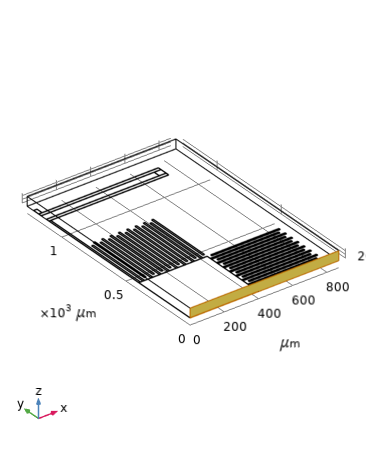
\includegraphics[width=0.3\textwidth]{y_symmetry_plane.png}%
            \label{fig:y-plane}}
        \hfil
        \subfloat[]{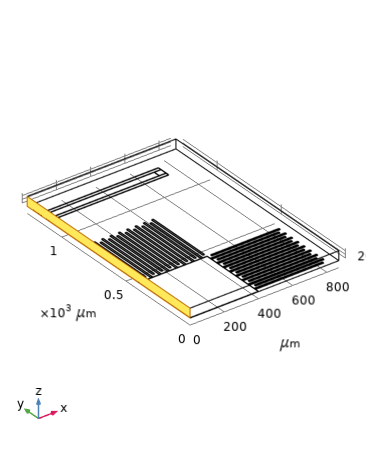
\includegraphics[width=0.3\textwidth]{x_symmetry_plane.png}%
            \label{fig:x-plane}}
        \hfil
        \subfloat[]{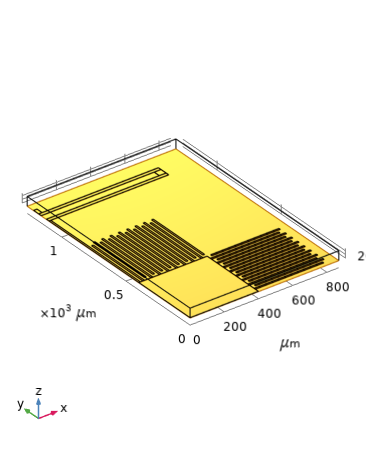
\includegraphics[width=0.3\textwidth]{z_symmetry_plane.png}%
            \label{fig:z-plane}}
        \caption{Symmetry planes, (a) \(y=0\), (b) \(x=0\) and (c) \(z=0\).}
        \label{fig:symmetry-planes}
    \end{figure*}
        The device was simulated using COMSOL Multiphysics 6.0.
        
        The only COMSOL module used for the simulation of the analysed system is \textit{Solid Mechanics}, because in this study we are not interested in evaluating the capacitance of the device, but only its mechanical properties.
        
        Following \cite{original}, the used materials are:
        
        \begin{itemize}
            \item Air (Built-in)
            \item Polycrystalline silicon (MEMS)
        \end{itemize}
        
        The polysilicon used is considered to be isotropic, with mass density \(\rho _{poly} =2320kg/m^3\) and Young's modulus of \(E_{poly}=169GPa\). The other default material properties are left unchanged.
        
         \subsection{Moving Mesh}
        The air domain was defined as a \textbf{Deforming Domain} in the \textit{Moving Mesh} section. In order to take into account the symmetries of the model, \textbf{Symmetry/Roller} were applied on the air domain boundaries, corresponding to the planes \(z=0, y=0\) and \(x=0\), see \ref{fig:symmetry-planes}. However, the Symmetry/Roller forces to zero the displacement of the moving mesh perpendicular to the selected boundary (\(\overset{\rightharpoonup}{u}\cdot\hat{n}=0\)), therefore, not all these three conditions could be enabled simultaneously. Depending on the type of simulation performed (acceleration along the X axis or Y axis), one of the three symmetry planes becomes, as a matter of fact, an antisymmetry plane and displacements of the moving mesh perpendicular to that plane must be allowed: for example, if an acceleration along X axis is simulated, the Symmetry/Roller associated to the plane \(x=0\) must be disabled.
        
        \subsection{Solid Mechanics}
        
        In the \textit{Solid Mechanics} module, similar boundary symmetries were defined: polysilicon boundaries that lay on one of the symmetry planes were included in the \textbf{Boundary Symmetry} or \textbf{Boundary Antisymmetry} object associated to that plane. Similarly to what was explained before, depending on the current simulation the symmetries and antisymmetries will change: if an X acceleration has to be simulated, the \(x=0\) plane becomes an antisymmetry plane, whereas the \(y=0\) plane is a symmetry plane; the opposite happens for Y acceleration simulations. The plane \(z=0\) will always be a symmetry plane for our studies, given that no accelerations along Z axis will be simulated. All these conditions are already defined inside the \textit{Solid Mechanics} module and they just need to be enabled/disabled. On the bottom boundaries of the fixed fingers and anchor domains, a \textbf{Fixed Constraint} condition is applied, as shown in figure \ref{fig:fixed-bound}. This prevents these domains from moving.
        
        \begin{figure}[!h]
            \centering
            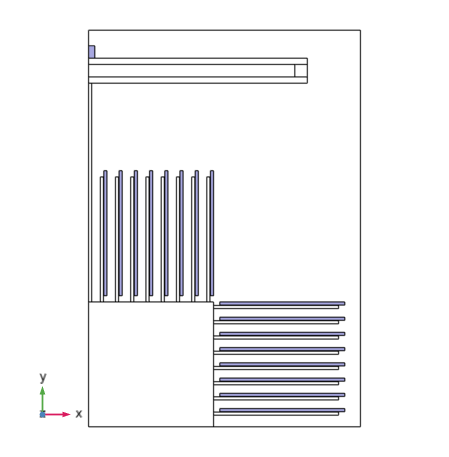
\includegraphics[width=1.0\linewidth]{fixed_boundaries.png}
            \caption{Fixed boundaries.}
            \label{fig:fixed-bound}
        \end{figure}
        
        All the other domains are set as \textbf{Free Linear Elastic Material}. To the \textit{polysilicon} domain, i.e. the whole structure, a \textbf{Body Load} was applied. The load was defined as a planar force per unit volume (\(N/m^3\)) with components:
        \begin{equation*}
            F_x=a_x g \rho_{poly}
        \end{equation*}
        \begin{equation*}
            F_y=a_y g \rho_{poly}
        \end{equation*}
        \begin{equation*}
            F_z=0
        \end{equation*}
        where \(g=9.81m/s^2\) is the gravity acceleration, whereas \(a_x\) and \(a_y\) are two model parameters. These are two pure numbers used to define the external acceleration as a multiple of \(g\).
        
        
        \iffalse
        \bigskip
        \subsection{Electrostatics}
        In the \textit{Electrostatics} module, after applying the \textbf{Charge Conservation} to all the domains, air included, one horizontal and one vertical fingers were defined as \textbf{Terminals} of type \textit{Voltage}, with an applied voltage of \(1mV\). The fixed fingers boundaries that face those terminals were defined as \textbf{Ground} boundaries. This was necessary in order to evaluate the total equivalent capacitance between one pair of vertical/horizontal movable and fixed fingers. To include in the capacitance evaluation all the capacitances of a single movable-fixed fingers pair (two longitudinal and one transverse, see section \ref{sssec:capacity}), the ground boundaries were selected as shown in figure \ref{fig:grounds}.
        
        \begin{figure}[!h]
            \centering
            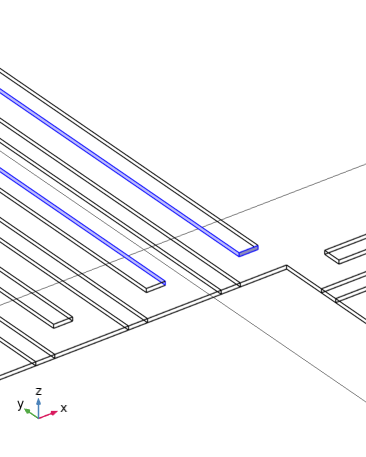
\includegraphics[width=1.0\linewidth]{grounds.png}
            \caption{Ground boundaries for one movable finger terminal.}
            \label{fig:grounds}
        \end{figure}
        
        The value of \(1mV\) applied to the terminals as a bias to sense the capacitance was chosen small enough so that electromechanical forces applied by the \textit{Multiphysics} module added only a negligible offset to the displacement of the mass. This way we can obtain the total capacitance of a single movable-fixed fingers pair, where, however, the cross capacitance between adjacent movable fingers was neglected.
        The total X or Y differential capacitance can be simply obtained using equation ...
        
        \bigskip
        \subsection{Multiphysics}        
        The module used in this section is the \textbf{Electromechanical Forces}, which couples the \textit{Solid Mechanics} and \textit{Electrostatics} modules. Its settings were left as default.
        
        \fi
        \subsection{Mesh and Study}
        The used mesh was of type \textit{physics-controlled} with element size set to \textbf{coarse}, in order to follow what done by the authors of \cite{original}.
        
        Given that our interest is in the steady state of the system in different conditions, 4 \textbf{stationary} studies were defined:
        \begin{itemize}
            \item Parametric sweep of the parameter \(a_x\) (X axis acceleration) from \(1g\) to \(50g\) in 10 steps. \(a_y\) is set to 0 and the geometrical parameters are set to their default values, as specified in table \ref{tab:size}.
            \item Parametric sweep of the parameter \(a_y\) (Y axis acceleration) from \(1g\) to \(50g\) in 10 steps. \(a_x\) is set to 0 and the geometrical parameters are set to their default values, as specified in table \ref{tab:size}.
            \item Parametric sweep of the thickness of the straight beam \(t_{bx}\) from \(1\mu m\) to \(30\mu m\) in 20 steps. \(a_y\) is set to 0 and \(a_x\) is set to \(1g\), given that we need to find the displacement sensitivity along the X axis. The other geometrical parameters are set to their default values.
            \item Parametric sweep of the width of the straight beam \(w_{bx}\) from \(4\mu m\) to \(20\mu m\) in 20 steps. \(a_y\) is set to 0 and \(a_x\) is set to \(1g\), given that we need to find the displacement sensitivity along the X axis. The other geometrical parameters are set to their default values.
        \end{itemize}
        In all four studies, the \textit{direct stationary solver} and the \textit{suggested direct solver} were set to \textbf{MUMPS}.
        
    \section{Simulation Results}
    \subsection{\(a_x\) parametric sweep}\label{sse:ax_sweep_results}
    The 3D plots for this simulation are presented in figures \ref{fig:disp_ax}, \ref{fig:disp_ax_det}, \ref{fig:stress_ax} and \ref{fig:stress_ax_det}.
    
    The maximum displacements along the X axis of the inertial mass are listed in table \ref{tab:max_x_disp}.
    
    \begin{table}[h]
        \caption{Maximum X displacement of the inertial mass for \(a_x\) accelerations between 1g and 50g.}
        \renewcommand{\arraystretch}{1.5}
        \centering
        \begin{tabular}{|c|c|}
            \hline
            \textbf{\(a_x\) [g]} & \textbf{Maximum X displacement [\(\mu\)m]} \\ \hline
            1.0000       & 0.0047630                 \\ \hline
            6.4444       & 0.030692                \\ \hline
            11.889       & 0.056615                \\ \hline
            17.333       & 0.082532                 \\ \hline
            22.778       & 0.10844                 \\ \hline
            28.222       & 0.13435                 \\ \hline
            33.667       & 0.16025                 \\ \hline
            39.111       & 0.18614                 \\ \hline
            44.556       & 0.21202                 \\ \hline
            50.000       & 0.23790                 \\ \hline
        \end{tabular}
        \label{tab:max_x_disp}
    \end{table}
    
    \begin{figure}[!h]
        \centering
        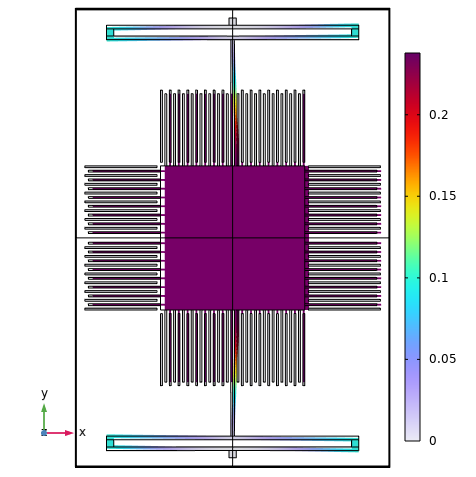
\includegraphics[width=1.0\linewidth]{displacement_ax}
        \caption{Displacement (\(\mu m\)) for acceleration \(a_x=50g\).}
        \label{fig:disp_ax}
    \end{figure}
    
    \begin{figure}[!h]
        \centering
        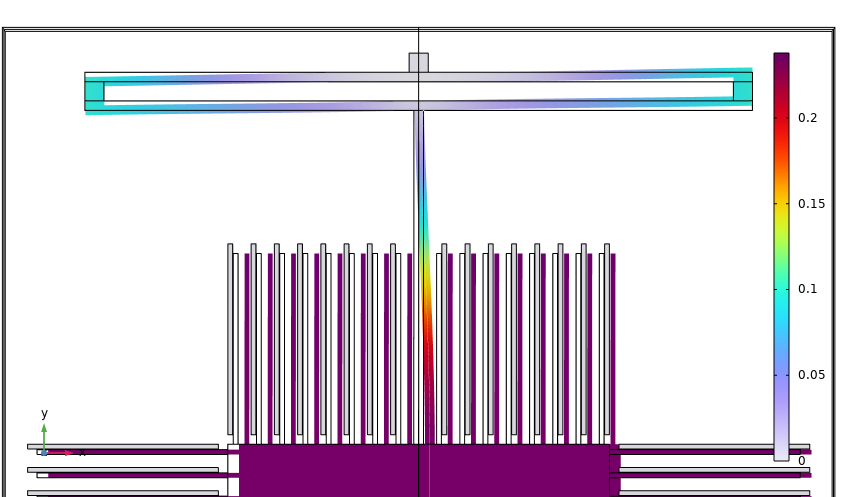
\includegraphics[width=1.0\linewidth]{displacement_ax_detail}
        \caption{Displacement (\(\mu m\)) for acceleration \(a_x=50g\), detail.}
        \label{fig:disp_ax_det}
    \end{figure}
    
    The maximum von Mises stress evaluated for different accelerations on the polysilicon structure is listed in table \ref{tab:max_x_stress}.
    
        \begin{table}[h]
        \caption{Maximum Von Mises stress of the polysilicon structure for \(a_x\) accelerations between 1g and 50g.}
        \renewcommand{\arraystretch}{1.5}
        \centering
        \begin{tabular}{|c|c|}
            \hline
            \textbf{\(a_x\) [g]} & \textbf{Maximum Von Mises stress [MPa]} \\ \hline
            1.0000       & 0.087655                 \\ \hline
            6.4444       & 0.56487                \\ \hline
            11.889       & 1.0420                \\ \hline
            17.333       & 1.5192                 \\ \hline
            22.778       & 1.9962                 \\ \hline
            28.222       & 2.4732                 \\ \hline
            33.667       & 2.9502                 \\ \hline
            39.111       & 3.4271                 \\ \hline
            44.556       & 3.9039                 \\ \hline
            50.000       & 4.3807                 \\ \hline
        \end{tabular}
        \label{tab:max_x_stress}
    \end{table}
    
    The maximum von Mises stress simulated for \(a_x=50g\) is \(4.3807\cdot10^6Pa\), which is almost identical to what is obtained in \cite{original} (\(4.5594\cdot10^6Pa\)). Therefore the conclusions are analogous: according to \cite{fracture}, the minimum fracture strength of polysilicon is \((2.9\pm 0.5)GPa\) (tensile stress), which is far higher then what we simulated at \(a_x=50g\), so there are no structural problems at this acceleration.
    
    \begin{figure}[!h]
        \centering
        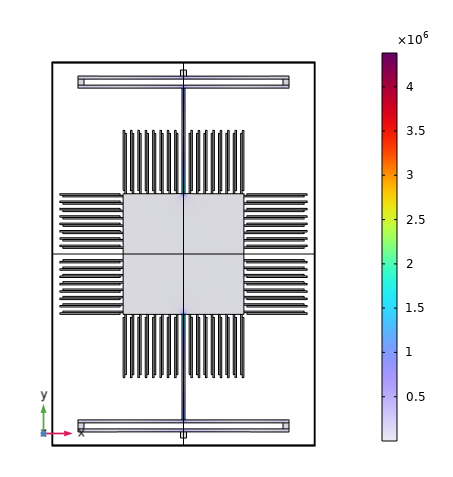
\includegraphics[width=1.0\linewidth]{stress_ax}
        \caption{Von Mises stress intensity (\(N/m^2\)) for acceleration \(a_x=50g\).}
        \label{fig:stress_ax}
    \end{figure}
    
    \begin{figure}[!h]
        \centering
        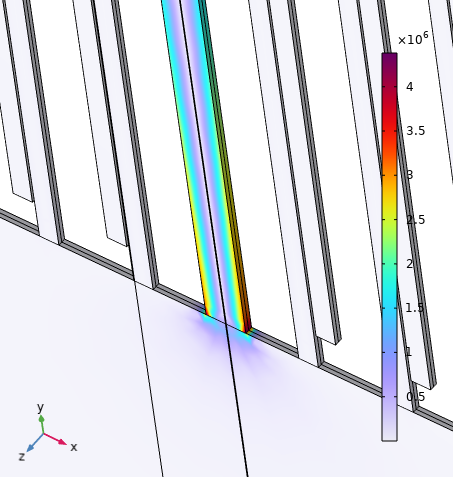
\includegraphics[width=1.0\linewidth]{stress_ax_detail}
        \caption{Von Mises stress intensity (\(N/m^2\)) for acceleration \(a_x=50g\), detail of the straight beam attachment to the central mass.}
        \label{fig:stress_ax_det}
    \end{figure}
    
    In figure \ref{plt:x_disp} we can see that the relationship between the x displacement and the x acceleration (therefore, the force) is quite linear, which means that the equivalent x stiffness is constant in the applied range of accelerations, as predicted by our model. The inverse of the mean slope of this curve multiplied by the total simulated inertial mass (\(\frac{m}{8}\)) gives us an equivalent x stiffness \(k_{x,reduced}=2.1411N/m\). Using equation \ref{eq:k_x_red}, we obtain \(k_x=17.1287N/m\).
    \begin{figure}[!h]
        \centering
        % This file was created with tikzplotlib v0.10.1.
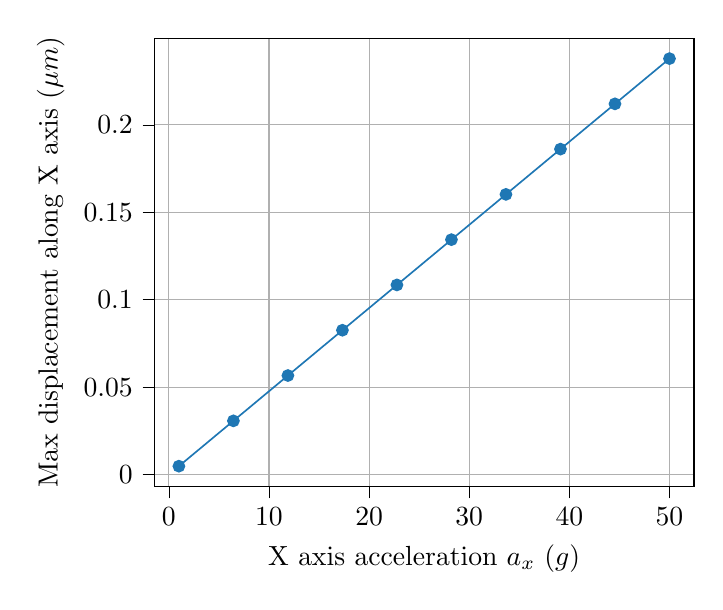
\begin{tikzpicture}

\definecolor{darkgray176}{RGB}{176,176,176}
\definecolor{steelblue31119180}{RGB}{31,119,180}

\begin{axis}[
tick align=outside,
tick pos=left,
x grid style={darkgray176},
xlabel={X axis acceleration $a_x$ $(g)$},
xmajorgrids,
xmin=-1.45, xmax=52.45,
xtick style={color=black},
y grid style={darkgray176},
ylabel={Max displacement along X axis $(\mu m)$},
ymajorgrids,
ymin=-0.00689383967282735, ymax=0.249556774730203,
ytick style={color=black},
yticklabel style={/pgf/number format/fixed}
]
\addplot [semithick, steelblue31119180, mark=*, mark size=2, mark options={solid}]
table {%
1 0.0047630064364013
6.44444444444444 0.0306917780422149
11.8888888888889 0.0566150225912782
17.3333333333333 0.0825324647766782
22.7777777777778 0.108443829876931
28.2222222222222 0.134348843785809
33.6666666666667 0.160247233043313
39.1111111111111 0.186138724864971
44.5555555555556 0.212023047171906
50 0.237899928620974
};
\end{axis}

\end{tikzpicture}

        \caption{Maximum displacement of the inertial mass along X axis for \(a_x\) accelerations between \(1g\) and \(50g\).}
        \label{plt:x_disp}
    \end{figure}
    
    As explained in section \ref{sssec:stiffness}, the x displacement sensitivity corresponds to the x displacement of the movable fingers for \(a_x=1g\). Considering the movable fingers as rigid bodies anchored to the central mass, we can evaluate the maximum displacement of the central mass, instead of the fingers'. The obtained sensitivity is \(S_x=0.004763\mu m\).
    
    \begin{table}[h]
        \caption{Comparison of simulated and theoretical values for the X equivalent stiffness and \(S_x\) sensitivity.}
        \renewcommand{\arraystretch}{1.5}
        \centering
        \begin{tabular}{|c|c|c|}
            \hline
            \textbf{Device Property} & \textbf{COMSOL} & \textbf{Theoretical}\\ \hline
            \(k_x\) [N/m]       & 17.1287   & 31.5335             \\ \hline
            \(S_x\) [\(\mu\)m]  & 0.004763  & 0.002587              \\ \hline
        \end{tabular}
        \label{tab:ax_sweep_comparison}
    \end{table}
    
    As we can see from this table, the difference with the predicted values is considerable: the simulated value is almost half of the stiffness obtained with our theoretical model. This is reasonable and it is due to the fact that we approximated the folded beam segments as fixed when applying accelerations along the x axis. As it is possible to notice from the displacement plot, this is not true and the two segments and the junction move as well. This implies that the total equivalent x stiffness is obtained from the series of two springs: the straight beam, with spring constant equal to the \(k_x\) calculated in section \ref{sssec:stiffness}, and the folded beam, with spring constant equal to the equivalent x stiffness of a folded beam structure. The fact that these springs are in series explains why the obtained stiffness is much smaller than the predicted one. 
    
    This x stiffness of the folded beam could be evaluated through analytical expressions, thanks to a more accurate model of the structure. However, this analysis goes beyond the scope of this report. On the other hand, it would be possible to retrieve an approximation of this stiffness value by using the inverse formula for springs in series:
    
    \begin{equation}\label{eq:kx_adjust}
        k_{x,COMSOL}=\frac{k_{x,straight}k_{x,folded,tot}}{k_{x,straight}+k_{x,folded,tot}}
    \end{equation}
    
    where \(k_{x,straight}=31.5335N/m\) is the total stiffness of the straight beams, \(k_{x,COMSOL}=17.1287N/m\) is the stiffness obtained with the simulation and \(k_{x,folded,tot}\) is the total x stiffness of all the folded beams combined.
    
    \begin{equation}\label{eq:kx_folded_tot}
        k_{x,folded,tot}=\frac{k_{x,COMSOL}k_{x,straight}}{k_{x,straight}-k_{x,COMSOL}}=37.4964N/m
    \end{equation}
    
    Therefore, the equivalent x stiffness of a single folded beam, supposing the four folded beams springs in parallel:
    
    \begin{equation}\label{eq:kx_folded}
        k_{x,folded}=\frac{k_{x,folded,tot}}{4}=9.3741N/m
    \end{equation}
    
    \bigskip
    \subsection{\(a_y\) parametric sweep}
    The 3D plots for this simulation are presented in figures \ref{fig:disp_ay}, \ref{fig:disp_ay_det}, \ref{fig:stress_ay} and \ref{fig:stress_ay_det}.
    
    The maximum displacements along the X axis of the inertial mass are listed in table \ref{tab:max_y_disp}.
    
    \begin{table}[h]
        \caption{Maximum Y displacement of the inertial mass for \(a_y\) accelerations between 1g and 50g.}
        \renewcommand{\arraystretch}{1.5}
        \centering
        \begin{tabular}{|c|c|}
            \hline
            \textbf{\(a_y\) [g]} & \textbf{Maximum Y displacement [\(\mu\)m]} \\ \hline
            1.0000       & 0.0024836                 \\ \hline
            6.4444       & 0.016005                \\ \hline
            11.889       & 0.029527                \\ \hline
            17.333       & 0.043049                 \\ \hline
            22.778       & 0.056571                 \\ \hline
            28.222       & 0.070092                 \\ \hline
            33.667       & 0.083614                 \\ \hline
            39.111       & 0.097136                 \\ \hline
            44.556       & 0.11066                 \\ \hline
            50.000       & 0.12418                 \\ \hline
        \end{tabular}
        \label{tab:max_y_disp}
    \end{table}
    
    \begin{figure}[!h]
        \centering
        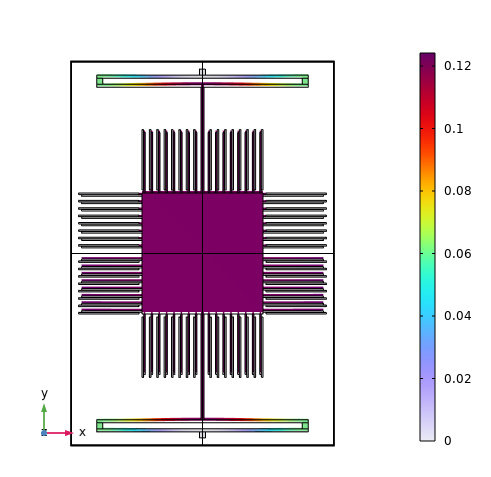
\includegraphics[width=1.0\linewidth]{displacement_ay}
        \caption{Displacement (\(\mu m\)) for acceleration \(a_y=50g\).}
        \label{fig:disp_ay}
    \end{figure}
    
    \begin{figure}[!h]
        \centering
        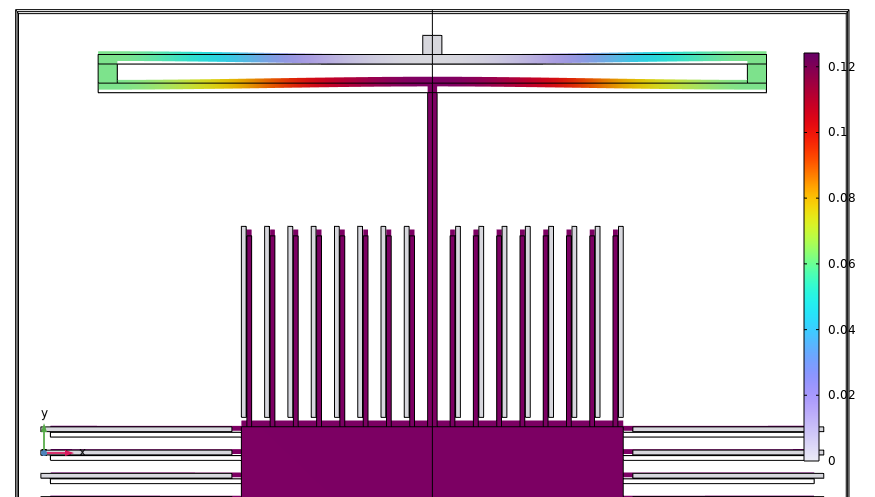
\includegraphics[width=1.0\linewidth]{displacement_ay_detail}
        \caption{Displacement (\(\mu m\)) for acceleration \(a_y=50g\), detail.}
        \label{fig:disp_ay_det}
    \end{figure}
    
    The maximum von Mises stress evaluated for different accelerations on the polysilicon structure is listed in table \ref{tab:max_y_stress}.
    
    \begin{table}[h]
        \caption{Maximum Von Mises stress of the polysilicon structure for \(a_y\) accelerations between 1g and 50g.}
        \renewcommand{\arraystretch}{1.5}
        \centering
        \begin{tabular}{|c|c|}
            \hline
            \textbf{\(a_y\) [g]} & \textbf{Maximum Von Mises stress [MPa]} \\ \hline
            1.0000       & 0.052332                 \\ \hline
            6.4444       & 0.33725                \\ \hline
            11.889       & 0.62217                \\ \hline
            17.333       & 0.90709                 \\ \hline
            22.778       & 1.1920                 \\ \hline
            28.222       & 1.4769                 \\ \hline
            33.667       & 1.7618                 \\ \hline
            39.111       & 2.0468                 \\ \hline
            44.556       & 2.3317                 \\ \hline
            50.000       & 2.6166                 \\ \hline
        \end{tabular}
        \label{tab:max_y_stress}
    \end{table}
    
    The maximum von Mises stress simulated for \(a_y=50g\) is \(2.6166\cdot10^6Pa\), which is almost identical to what is obtained in \cite{original} (\(2.5348\cdot10^6Pa\)). The same conclusions as before apply.
    
    \begin{figure}[!h]
        \centering
        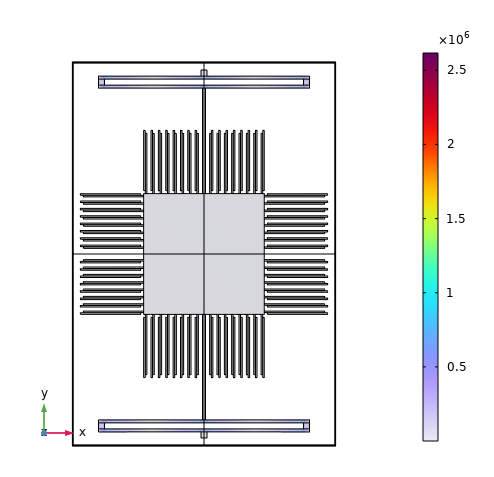
\includegraphics[width=1.0\linewidth]{stress_ay}
        \caption{Von Mises stress intensity (\(N/m^2\)) for acceleration \(a_y=50g\).}
        \label{fig:stress_ay}
    \end{figure}
    
    \begin{figure}[!h]
        \centering
        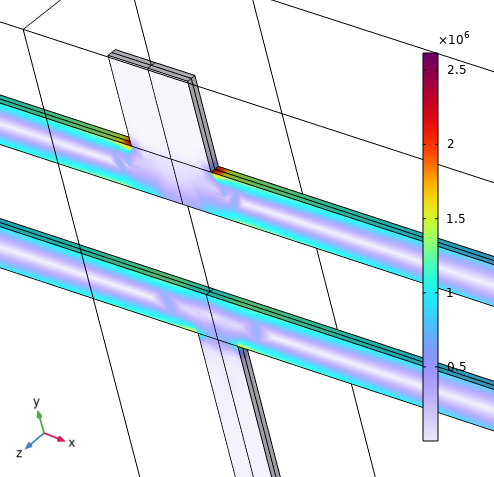
\includegraphics[width=1.0\linewidth]{stress_ay_detail}
        \caption{Von Mises stress intensity (\(N/m^2\)) for acceleration \(a_y=50g\), detail of the folded beam attachment to the anchor.}
        \label{fig:stress_ay_det}
    \end{figure}
    
    In figure \ref{plt:y_disp} we can see that the relationship between the y displacement and the y acceleration (therefore, the force) is here as well quite linear, which means that the equivalent y stiffness is constant in the applied range of accelerations, as predicted by our model. The inverse of the mean slope of this curve multiplied by the total simulated inertial mass (\(\frac{m}{8}\)) gives us an equivalent y stiffness \(k_{y,reduced}=4.104N/m\). Using equation \ref{eq:k_y_red}, we obtain \(k_y=32.832N/m\).    
    \begin{figure}[!h]
        \centering
        % This file was created with tikzplotlib v0.10.1.
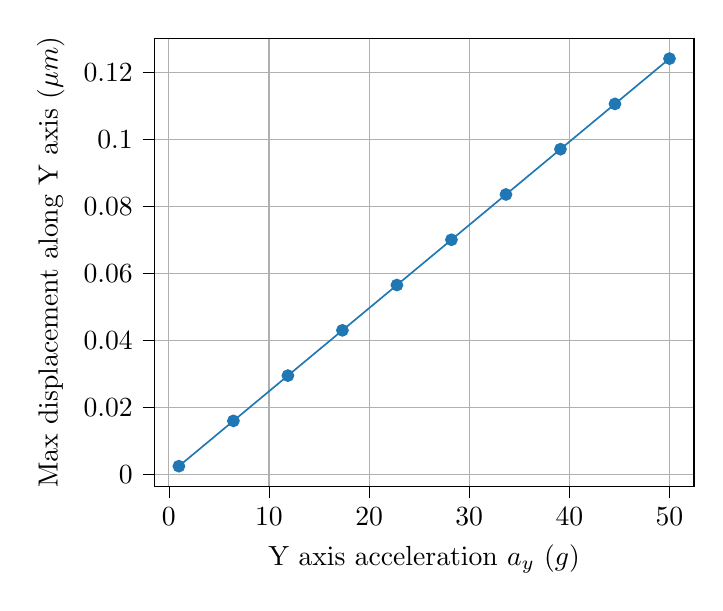
\begin{tikzpicture}

\definecolor{darkgray176}{RGB}{176,176,176}
\definecolor{steelblue31119180}{RGB}{31,119,180}

\begin{axis}[
tick align=outside,
tick pos=left,
x grid style={darkgray176},
xlabel={Y axis acceleration $a_y$ $(g)$},
xmajorgrids,
xmin=-1.45, xmax=52.45,
xtick style={color=black},
y grid style={darkgray176},
ylabel={Max displacement along Y axis $(\mu m)$},
ymajorgrids,
ymin=-0.00360120181423542, ymax=0.130264149841756,
ytick style={color=black},
yticklabel style={/pgf/number format/fixed}
]
\addplot [semithick, steelblue31119180, mark=*, mark size=2, mark options={solid}]
table {%
1 0.00248358689740058
6.44444444444444 0.0160053380318978
11.8888888888889 0.029527089571949
17.3333333333333 0.0430488415108165
22.7777777777778 0.0565705938416867
28.2222222222222 0.0700923465602717
33.6666666666667 0.0836140996563783
39.1111111111111 0.0971358531217806
44.5555555555556 0.110657606948991
50 0.12417936113012
};
\end{axis}

\end{tikzpicture}

        \caption{Maximum displacement along Y axis for \(a_y\) accelerations between \(1g\) and \(50g\).}
        \label{plt:y_disp}
    \end{figure}
    
    As explained in section \ref{sssec:stiffness}, the y displacement sensitivity corresponds to the y displacement of the movable fingers for \(a_y=1g\). Considering the movable fingers as rigid bodies anchored to the central mass, we can evaluate the maximum displacement of the central mass, instead of the fingers'. The obtained sensitivity is \(S_y=0.0024836\mu m\).
    
    \begin{table}[h]
        \caption{Comparison of simulated and theoretical values for the Y equivalent stiffness and \(S_y\) sensitivity.}
        \renewcommand{\arraystretch}{1.5}
        \centering
        \begin{tabular}{|c|c|c|}
            \hline
            \textbf{Device Property} & \textbf{COMSOL} & \textbf{Theoretical}\\ \hline
            \(k_y\) [N/m]       & 32.832   & 31.5335             \\ \hline
            \(S_y\) [\(\mu\)m]  & 0.0024836  & 0.002587              \\ \hline
        \end{tabular}
        \label{tab:ay_sweep_comparison}
    \end{table}
    
    Here, simulated results are quite similar to the predicted values, since no big approximation was made in the model of the Y springs.
    
    \bigskip
    \subsection{\(t_{bx}\) parametric sweep}\label{sse:tbx_sweep_study}
    Through this simulation, it was possible to verify that the \(S_x\) sensitivity is inversely proportional to the thickness of the straight beam, as anticipated by equation \ref{eq:x_sens}.
    
    \begin{figure}[!h]
        \centering
        % This file was created with tikzplotlib v0.10.1.
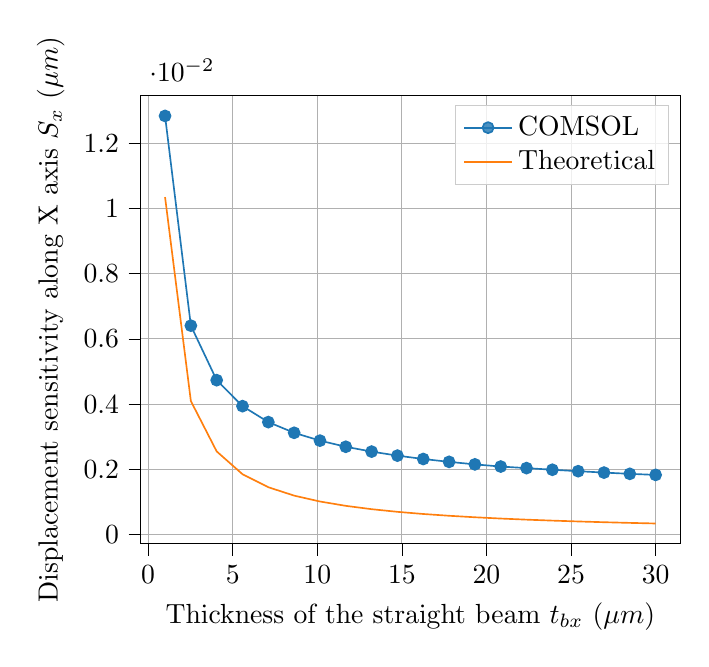
\begin{tikzpicture}

\definecolor{darkgray176}{RGB}{176,176,176}
\definecolor{darkorange25512714}{RGB}{255,127,14}
\definecolor{lightgray204}{RGB}{204,204,204}
\definecolor{steelblue31119180}{RGB}{31,119,180}

\begin{axis}[
legend cell align={left},
legend style={fill opacity=0.8, draw opacity=1, text opacity=1, draw=lightgray204},
tick align=outside,
tick pos=left,
x grid style={darkgray176},
xlabel={Thickness of the straight beam $t_{bx}$ $(\mu m)$},
xmajorgrids,
xmin=-0.45, xmax=31.45,
xtick style={color=black},
y grid style={darkgray176},
ylabel={Displacement sensitivity along X axis $S_x$ $(\mu m)$},
ymajorgrids,
ymin=-0.000279519677280009, ymax=0.0134576778770814,
ytick style={color=black},
yticklabel style={/pgf/number format/fixed}
]
\addplot [semithick, steelblue31119180, mark=*, mark size=2, mark options={solid}]
table {%
1 0.0128332598064286
2.52631578947368 0.00640666964698149
4.05263157894737 0.00473612859955784
5.57894736842105 0.00394044814011472
7.10526315789474 0.00345147151342667
8.63157894736842 0.00312394969900687
10.1578947368421 0.00288369021827935
11.6842105263158 0.00269594951779226
13.2105263157895 0.00254756582035972
14.7368421052632 0.00242414363456502
16.2631578947368 0.00232099790826183
17.7894736842105 0.00223353935316908
19.3157894736842 0.00215663208102844
20.8421052631579 0.0020895279511115
22.3684210526316 0.00204198639426458
23.8947368421053 0.00199169981392245
25.4210526315789 0.00194719304147826
26.9473684210526 0.00190465069891878
28.4736842105263 0.00186665849987364
30 0.00183358499480313
};
\addlegendentry{COMSOL}
\addplot [semithick, darkorange25512714]
table {%
1 0.0103469518011834
2.52631578947368 0.00409566842130178
4.05263157894737 0.00255314395094137
5.57894736842105 0.00185464230398571
7.10526315789474 0.0014562376609073
8.63157894736842 0.00119873222086881
10.1578947368421 0.00101861183534966
11.6842105263158 0.000885549928930114
13.2105263157895 0.000783235395308706
14.7368421052632 0.000702114586508876
16.2631578947368 0.000636220337289596
17.7894736842105 0.000581633385273625
19.3157894736842 0.000535673254012221
20.8421052631579 0.000496444657127488
22.3684210526316 0.000462569609935259
23.8947368421053 0.0004330222119438
25.4210526315789 0.000407022948700798
26.9473684210526 0.000383968914497041
28.4736842105263 0.000363386477305888
30 0.000344898393372781
};
\addlegendentry{Theoretical}
\end{axis}

\end{tikzpicture}

        \caption{Displacement sensitivity along X axis \(S_x\) for thicknesses of the straight beam \(t_{bx}\) between \(1\mu m\) and \(30\mu m\). The orange curve is the plot of equation \ref{eq:x_sens} against \(t_{bx}\).}
        \label{plt:tbx_sweep}
    \end{figure}
    
    A comparison between the theoretical and simulated values is presented in table \ref{tab:tbx_sweep}.
    
    \begin{table}[h]
        \caption{Displacement sensitivity along X axis for different \(t_{bx}\) values.}
        \renewcommand{\arraystretch}{1.2}
        \centering
        \begin{tabular}{|c|c|c|}
            \hline
            \textbf{\(t_{bx}\) [\(\mu\)m]} & \textbf{COMSOL \(S_x\) [\(\mu\)m]} & \textbf{Theoretical \(S_x\) [\(\mu\)m]}\\ \hline
            1.0000       & 0.012833      & 0.01034695                \\ \hline
            2.5263       & 0.0064067     & 0.00409567                \\ \hline
            4.0526       & 0.0047361     & 0.00255314                \\ \hline
            5.5789       & 0.0039404     & 0.00185464                \\ \hline
            7.1053       & 0.0034515     & 0.00145624                \\ \hline
            8.6316       & 0.0031239     & 0.00119873               \\ \hline
            10.158       & 0.0028837     & 0.00101861                \\ \hline
            11.684       & 0.0026959     & 0.00088555                \\ \hline
            13.211       & 0.0025476     & 0.00078324                \\ \hline
            14.737       & 0.0024241     & 0.00070211                \\ \hline
            16.263       & 0.0023210     & 0.00063622                \\ \hline
            17.789       & 0.0022335     & 0.00058163               \\ \hline
            19.316       & 0.0021566     & 0.00053567                \\ \hline
            20.842       & 0.0020895     & 0.00049644                \\ \hline
            22.368       & 0.0020420     & 0.00046257               \\ \hline
            23.895       & 0.0019917     & 0.00043302               \\ \hline
            25.421       & 0.0019472     & 0.00040702               \\ \hline
            26.947       & 0.0019047     & 0.00038397               \\ \hline
            28.474       & 0.0018667     & 0.00036339               \\ \hline
            30.000       & 0.0018336     & 0.0003449               \\ \hline
        \end{tabular}
        \label{tab:tbx_sweep}
    \end{table}
    
    As already discussed in section \ref{sse:ax_sweep_results}, the theoretical model differs from the COMSOL simulation results because the equivalent x stiffness of the folded beams was not considered for simplicity. It is possible to compare the relative errors made for the x displacement sensitivity evaluation between the COMSOL simulation and the theoretical model with and without this approximation. The analytical expression for the displacement sensitivity considering the x stiffness of the folded beams can be obtained from equation \ref{eq:x_sens}, replacing \(k_x\) with \ref{eq:kx_adjust}, where \(k_{x,folded,tot}\) is evaluated in equation \ref{eq:kx_folded_tot}. The result is shown in figure \ref{plt:tbx_errors}. The theoretical adjusted sensitivity values can be found in table \ref{tab:tbx_sweep_adj}.
    
    \begin{figure}[!h]
        \centering
        % This file was created with tikzplotlib v0.10.1.
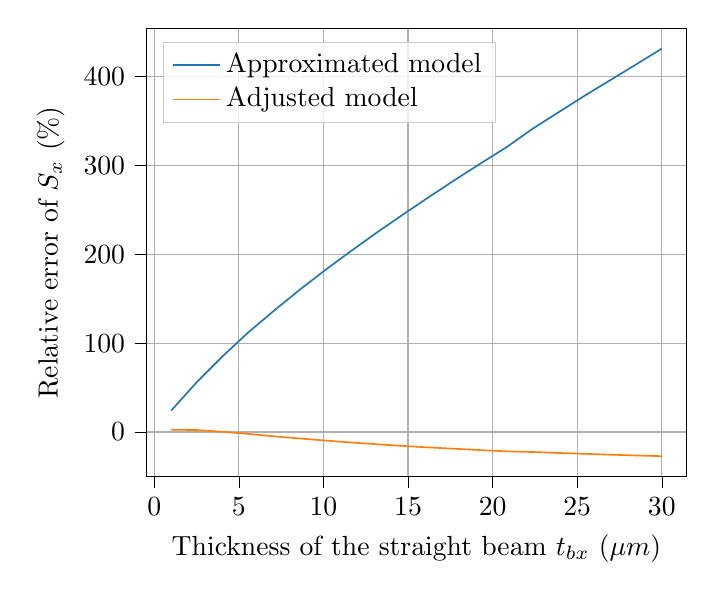
\begin{tikzpicture}

\definecolor{darkgray176}{RGB}{176,176,176}
\definecolor{darkorange25512714}{RGB}{255,127,14}
\definecolor{lightgray204}{RGB}{204,204,204}
\definecolor{steelblue31119180}{RGB}{31,119,180}

\begin{axis}[
legend cell align={left},
legend style={
  fill opacity=0.8,
  draw opacity=1,
  text opacity=1,
  at={(0.03,0.97)},
  anchor=north west,
  draw=lightgray204
},
tick align=outside,
tick pos=left,
x grid style={darkgray176},
xlabel={Thickness of the straight beam $t_{bx}$ $(\mu m)$},
xmajorgrids,
xmin=-0.45, xmax=31.45,
xtick style={color=black},
y grid style={darkgray176},
ylabel={Relative error of $S_x$ (\%)},
ymajorgrids,
ymin=-50.1906666724258, ymax=454.574347347927,
ytick style={color=black}
]
\addplot [semithick, steelblue31119180]
table {%
1 24.0293765064295
2.52631578947368 56.425496108525
4.05263157894737 85.5018240476251
5.57894736842105 112.464049355853
7.10526315789474 137.012927634097
8.63157894736842 160.604465669798
10.1578947368421 183.100011035062
11.6842105263158 204.43788991654
13.2105263157895 225.261835154375
14.7368421052632 245.263249211014
16.2631578947368 264.810392284797
17.7894736842105 284.011545712482
19.3157894736842 302.602158102005
20.8421052631579 320.898466951354
22.3684210526316 341.444130873702
23.8947368421053 359.953267750834
25.4210526315789 378.398834191938
26.9473684210526 396.042941760967
28.4736842105263 413.684084700362
30 431.630483074275
};
\addlegendentry{Approximated model}
\addplot [semithick, darkorange25512714]
table {%
1 2.48296698045118
2.52631578947368 2.16261434111588
4.05263157894737 0.160770403394094
5.57894736842105 -2.22273420012844
7.10526315789474 -4.96056066161511
8.63157894736842 -7.41424386121537
10.1578947368421 -9.71523911468818
11.6842105263158 -11.923914944881
13.2105263157895 -13.8933838764247
14.7368421052632 -15.7551338387264
16.2631578947368 -17.4492992555728
17.7894736842105 -18.9870721325488
19.3157894736842 -20.4504733540858
20.8421052631579 -21.7940470073831
22.3684210526316 -22.5919861612564
23.8947368421053 -23.6429935251236
25.4210526315789 -24.5977046685406
26.9473684210526 -25.5807299264075
28.4736842105263 -26.473875345906
30 -27.2468023987734
};
\addlegendentry{Adjusted model}
\end{axis}

\end{tikzpicture}

        \caption{Relative error of \(S_x\) between the COMSOL simulation and the theoretical model with and without approximation on the stiffness of the folded beams.}
        \label{plt:tbx_errors}
    \end{figure}
    
     \begin{table}[!h]
        \caption{Displacement sensitivity along X axis for different \(t_{bx}\) values. Adjusted model inclusive of folded beams x stiffness.}
        \renewcommand{\arraystretch}{1.2}
        \centering
        \begin{tabular}{|c|c|c|}
            \hline
            \textbf{\(t_{bx}\) [\(\mu\)m]} & \textbf{COMSOL \(S_x\) [\(\mu\)m]} & \textbf{Theoretical adjusted \(S_x\) [\(\mu\)m]}\\ \hline
            1.0000       & 0.012833      & 0.01252233                 \\ \hline
            2.5263       & 0.0064067     & 0.00627105                 \\ \hline
            4.0526       & 0.0047361     & 0.00472853                \\ \hline
            5.5789       & 0.0039404     & 0.00403002                 \\ \hline
            7.1053       & 0.0034515     & 0.00363162                 \\ \hline
            8.6316       & 0.0031239     & 0.00337411               \\ \hline
            10.158       & 0.0028837     & 0.00319399                 \\ \hline
            11.684       & 0.0026959     & 0.00306093                 \\ \hline
            13.211       & 0.0025476     & 0.00295862                 \\ \hline
            14.737       & 0.0024241     & 0.0028775                  \\ \hline
            16.263       & 0.0023210     & 0.0028116                  \\ \hline
            17.789       & 0.0022335     & 0.00275702               \\ \hline
            19.316       & 0.0021566     & 0.00271106                 \\ \hline
            20.842       & 0.0020895     & 0.00267183                 \\ \hline
            22.368       & 0.0020420     & 0.00263795                \\ \hline
            23.895       & 0.0019917     & 0.0026084                 \\ \hline
            25.421       & 0.0019472     & 0.00258241                \\ \hline
            26.947       & 0.0019047     & 0.00255935               \\ \hline
            28.474       & 0.0018667     & 0.00253877                \\ \hline
            30.000       & 0.0018336     & 0.00252028               \\ \hline
        \end{tabular}
        \label{tab:tbx_sweep_adj}
    \end{table}
    
    \newpage
    \subsection{\(w_{bx}\) parametric sweep}
    Through this simulation, it was possible to verify that the \(S_x\) sensitivity is inversely proportional to the cubic power of the width of the straight beam, as anticipated by equation \ref{eq:x_sens}.
    
    \begin{figure}[!h]
        \centering
        % This file was created with tikzplotlib v0.10.1.
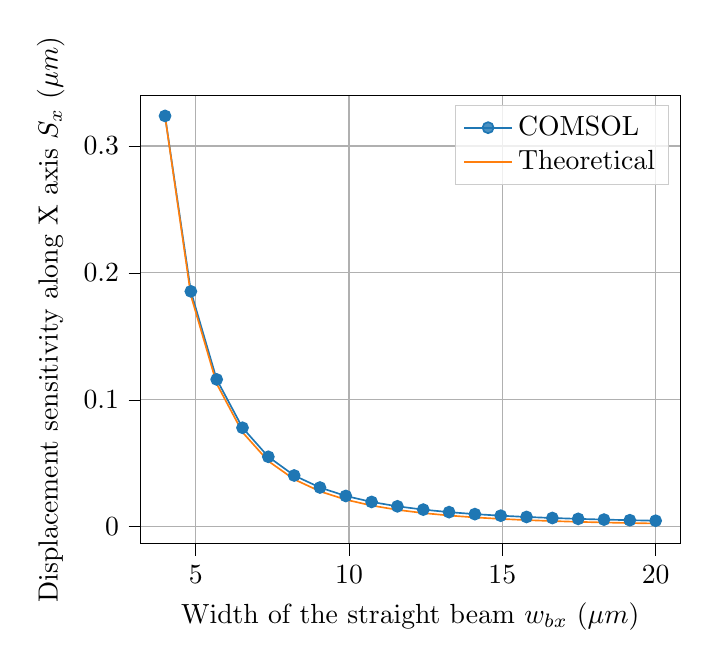
\begin{tikzpicture}

\definecolor{darkgray176}{RGB}{176,176,176}
\definecolor{darkorange25512714}{RGB}{255,127,14}
\definecolor{lightgray204}{RGB}{204,204,204}
\definecolor{steelblue31119180}{RGB}{31,119,180}

\begin{axis}[
legend cell align={left},
legend style={fill opacity=0.8, draw opacity=1, text opacity=1, draw=lightgray204},
tick align=outside,
tick pos=left,
x grid style={darkgray176},
xlabel={Width of the straight beam $w_{bx}$ $(\mu m)$},
xmajorgrids,
xmin=3.2, xmax=20.8,
xtick style={color=black},
y grid style={darkgray176},
ylabel={Displacement sensitivity along X axis $S_x$ $(\mu m)$},
ymajorgrids,
ymin=-0.0134675669737488, ymax=0.339727141355234,
ytick style={color=black},
yticklabel style={/pgf/number format/fixed}
]
\addplot [semithick, steelblue31119180, mark=*, mark size=2, mark options={solid}]
table {%
4 0.32367283643119
4.84210526315789 0.18546127408612
5.68421052631579 0.116082557457634
6.52631578947368 0.0780035629853383
7.36842105263158 0.0551301571837829
8.21052631578947 0.0404081976056517
9.05263157894737 0.0309172983004433
9.89473684210526 0.024271410579959
10.7368421052632 0.0195614427781789
11.578947368421 0.0161055753189082
12.4210526315789 0.0135172073511395
13.2631578947368 0.0115247492088279
14.1052631578947 0.0099634737030334
14.9473684210526 0.00873159723733105
15.7894736842105 0.00773212470221577
16.6315789473684 0.00691234980446039
17.4736842105263 0.00623234919973695
18.3157894736842 0.00566194465532576
19.1578947368421 0.00517984298973994
20 0.00476300643882209
};
\addlegendentry{COMSOL}
\addplot [semithick, darkorange25512714]
table {%
4 0.323342243786982
4.84210526315789 0.182280303290451
5.68421052631579 0.112676139314887
6.52631578947368 0.0744454516509991
7.36842105263158 0.051727217495858
8.21052631578947 0.0373877585619265
9.05263157894737 0.0278944552068989
9.89473684210526 0.0213613982463896
10.7368421052632 0.0167190933361597
11.578947368421 0.013330154471134
12.4210526315789 0.010798594063341
13.2631578947368 0.00886955032507853
14.1052631578947 0.00737392714574238
14.9473684210526 0.00619652497446269
15.7894736842105 0.00525701795587535
16.6315789473684 0.00449823330433275
17.4736842105263 0.00387872485756919
18.3157894736842 0.00336794889337621
19.1578947368421 0.00294305971187176
20 0.00258673795029586
};
\addlegendentry{Theoretical}
\end{axis}

\end{tikzpicture}

        \caption{Displacement sensitivity along X axis \(S_x\) for thicknesses of the straight beam \(w_{bx}\) between \(4 \mu m\) and \(20\mu m\). The orange curve is the plot of equation \ref{eq:x_sens} against \(w_{bx}\).}.
        \label{plt:wbx_sweep}
    \end{figure}
    
    
    A comparison between the theoretical and simulated values is presented in table \ref{tab:wbx_sweep}.
    
    \begin{table}[h]
        \caption{Displacement sensitivity along X axis for different \(w_{bx}\) values.}
        \renewcommand{\arraystretch}{1.2}
        \centering
        \begin{tabular}{|c|c|c|}
            \hline
            \textbf{\(w_{bx}\) [\(\mu\)m]} & \textbf{COMSOL \(S_x\) [\(\mu\)m]} & \textbf{Theoretical \(S_x\) [\(\mu\)m]}\\ \hline
            4.0000       & 0.32367      & 0.32334224                 \\ \hline
            4.8421       & 0.18546     & 0.1822803                  \\ \hline
            5.6842       & 0.11608     & 0.11267614                 \\ \hline
            6.5263       & 0.078004     & 0.07444545                 \\ \hline
            7.3684       & 0.055130     & 0.05172722                 \\ \hline
            8.2105       & 0.040408     & 0.03738776                \\ \hline
            9.0526       & 0.030917     & 0.02789446                   \\ \hline
            9.8947       & 0.024271     & 0.0213614                 \\ \hline
            10.737       & 0.019561     & 0.01671909                 \\ \hline
            11.579       & 0.016106     & 0.01333015                 \\ \hline
            12.421       & 0.013517     & 0.01079859                \\ \hline
            13.263       & 0.011525     & 0.00886955                \\ \hline
            14.105       & 0.0099635     & 0.00737393                 \\ \hline
            14.947       & 0.0087316     & 0.00619652                 \\ \hline
            15.789       & 0.0077321     & 0.00525702                \\ \hline
            16.632       & 0.0069123     & 0.00449823                \\ \hline
            17.474       & 0.0062323     & 0.00387872               \\ \hline
            18.316       & 0.0056619     & 0.00336795               \\ \hline
            19.158       & 0.0051798     & 0.00294306               \\ \hline
            20.000       & 0.0047630     & 0.00258674               \\ \hline
        \end{tabular}
        \label{tab:wbx_sweep}
    \end{table}
    
    Conclusions analogous to the ones of the previous study can be drawn. The model can be adjusted by considering the equivalent x stiffness of the folded beams. The improvement obtained in the relative error made in the evaluation of the x displacement sensitivity is shown in figure \ref{plt:wbx_errors}. The new adjusted values are listed in table \ref{tab:wbx_sweep_adj}.
    
    \begin{figure}[!h]
        \centering
        % This file was created with tikzplotlib v0.10.1.
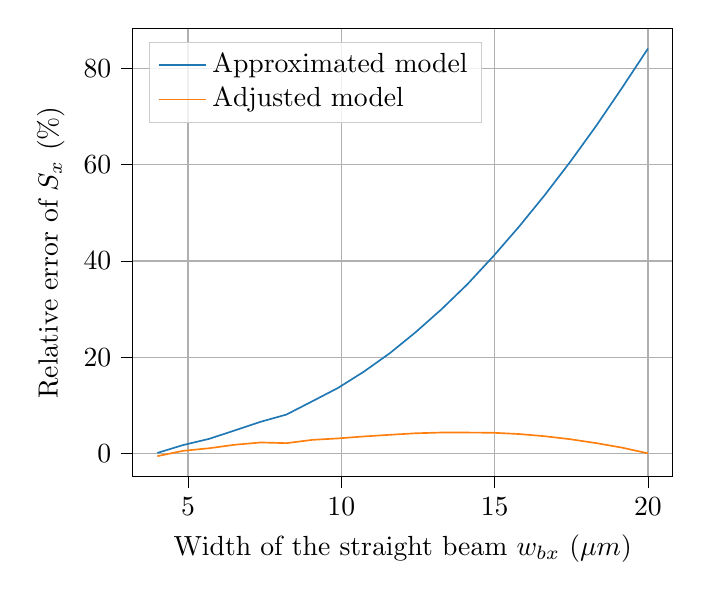
\begin{tikzpicture}

\definecolor{darkgray176}{RGB}{176,176,176}
\definecolor{darkorange25512714}{RGB}{255,127,14}
\definecolor{lightgray204}{RGB}{204,204,204}
\definecolor{steelblue31119180}{RGB}{31,119,180}

\begin{axis}[
legend cell align={left},
legend style={
  fill opacity=0.8,
  draw opacity=1,
  text opacity=1,
  at={(0.03,0.97)},
  anchor=north west,
  draw=lightgray204
},
tick align=outside,
tick pos=left,
x grid style={darkgray176},
xlabel={Width of the straight beam $w_{bx}$ $(\mu m)$},
xmajorgrids,
xmin=3.2, xmax=20.8,
xtick style={color=black},
y grid style={darkgray176},
ylabel={Relative error of $S_x$ (\%)},
ymajorgrids,
ymin=-4.80164993025062, ymax=88.3666974186229,
ytick style={color=black}
]
\addplot [semithick, steelblue31119180]
table {%
4 0.102242330088252
4.84210526315789 1.74509847649337
5.68421052631579 3.0231938753491
6.52631578947368 4.77948787391307
7.36842105263158 6.57862505014387
8.21052631578947 8.07868446759774
9.05263157894737 10.8367167278345
9.89473684210526 13.6227614878218
10.7368421052632 17.000619500532
11.578947368421 20.8206202995198
12.4210526315789 25.1756226028311
13.2631578947368 29.9361161099888
14.1052631578947 35.1176043119195
14.9473684210526 40.9111925363973
15.7894736842105 47.0819534404328
16.6315789473684 53.6681033818842
17.4736842105263 60.6803634853024
18.3157894736842 68.1125466737689
19.1578947368421 76.0019672331285
20 84.1317725391286
};
\addlegendentry{Approximated model}
\addplot [semithick, darkorange25512714]
table {%
4 -0.566725050756373
4.84210526315789 0.545165205125279
5.68421052631579 1.07184958894958
6.52631578947368 1.80463808678274
7.36842105263158 2.27736159074593
8.21052631578947 2.13596909129697
9.05263157894737 2.81830757511913
9.89473684210526 3.12119895080717
10.7368421052632 3.52995694417206
11.578947368421 3.86983223123619
12.4210526315789 4.18707945448764
13.2631578947368 4.34422110611191
14.1052631578947 4.33710908803487
14.9473684210526 4.29638864495508
15.7894736842105 4.03266976200549
16.6315789473684 3.57727994710352
17.4736842105263 2.94414604694294
18.3157894736842 2.13974547854072
19.1578947368421 1.19959739614878
20 0.0186032898343824
};
\addlegendentry{Adjusted model}
\end{axis}

\end{tikzpicture}

        \caption{Relative error of \(S_x\) between the COMSOL simulation and the theoretical model with and without approximation on the stiffness of the folded beams.}
        \label{plt:wbx_errors}
    \end{figure}
    
    \begin{table}[h]
        \caption{Displacement sensitivity along X axis for different \(w_{bx}\) values. Adjusted model inclusive of folded beams x stiffness.}
        \renewcommand{\arraystretch}{1.2}
        \centering
        \begin{tabular}{|c|c|c|}
            \hline
            \textbf{\(w_{bx}\) [\(\mu\)m]} & \textbf{COMSOL \(S_x\) [\(\mu\)m]} & \textbf{Theoretical adjusted \(S_x\) [\(\mu\)m]}\\ \hline
            4.0000       & 0.32367      & 0.32551763                  \\ \hline
            4.8421       & 0.18546     & 0.18445569                   \\ \hline
            5.6842       & 0.11608     & 0.11485152                  \\ \hline
            6.5263       & 0.078004     & 0.07662083                  \\ \hline
            7.3684       & 0.055130     & 0.0539026                   \\ \hline
            8.2105       & 0.040408     & 0.03956314                \\ \hline
            9.0526       & 0.030917     & 0.03006984                    \\ \hline
            9.8947       & 0.024271     & 0.02353678                  \\ \hline
            10.737       & 0.019561     & 0.01889448                  \\ \hline
            11.579       & 0.016106     & 0.01550554                  \\ \hline
            12.421       & 0.013517     & 0.01297398                 \\ \hline
            13.263       & 0.011525     & 0.01104493                \\ \hline
            14.105       & 0.0099635     & 0.00954931                  \\ \hline
            14.947       & 0.0087316     & 0.00837191                  \\ \hline
            15.789       & 0.0077321     & 0.0074324                  \\ \hline
            16.632       & 0.0069123     & 0.00667362                 \\ \hline
            17.474       & 0.0062323     & 0.00605411                \\ \hline
            18.316       & 0.0056619     & 0.00554333               \\ \hline
            19.158       & 0.0051798     & 0.00511844               \\ \hline
            20.000       & 0.0047630     & 0.00476212               \\ \hline
        \end{tabular}
        \label{tab:wbx_sweep_adj}
    \end{table}
    
    \section{Conclusions}
    The obtained results are coherent with the reference paper, from which the design idea of this dual-axis accelerometer was taken \cite{original}. In particular, the maximum stress of the polysilicon structure and the displacement sensitivities to input accelerations present negligible differences.
    
    However, the theoretical model proposed in \cite{original} is not very accurate for the prediction of the device stiffness along X axis, due to approximating the x stiffness of the folded beams as infinite, which turns out not to be true. Adjustments were made in order to compensate for this error. Nevertheless, the approximated model effectively managed to predict the dependency of the displacement sensitivity \(S_x\) as a function of the straight beam thickness \(t_{bx}\) and width \(w_{bx}\). This result can be helpful in the design and optimization of dual-axis accelerometers with T-shape beams.
    
    \printbibliography
\end{document}